\pagestyle{chapter-fancy-style}
\chapter{Manufacture and assembly}
%===============================================================================
\section{Architecture}
Overview of the ROV system is shown in Fig.~\ref{fig:systemBlockDiagram}, while Fig.~\ref{fig:rovGAsInternal} and Fig.~\ref{fig:rovGAsExternal} show the general dimensions of the vehicle and location of its major components. The ROV is based around an Arduino Uno R3, which is controlled and powered through its serial port connected to a~laptop. To overcome range limitations of ordinary USB cables, a~USB range extender is used, which transmits the USB signal and power over a~CAT5 cable.

The ROV houses one camera, which is operated over the same USB bus as the Arduino (the USB signal is split using an on-board USB hub). The camera field of view can be illuminated using three LED lights. Only one additional sensor, a~\unit[30]{PSI} pressure transducer, is present on board.

The ROV carries four \unit[750]{kV} brushless DC motors driven by four electronic speed controllers (ESCs). These enable forward/backward and up/down motion, as well as give control of yaw and roll. Preliminary study revealed that incorporating two additional motors, which would allow sideways motion, would require too big an investment. It would also increase the ROV displacement, thus making the vehicle larger than desired. The selected ESCs (chosen due to their low cost) can only provide thrust in one direction; a~custom printed circuit board (PCB) is used to reverse the thrust of individual motors.

The power to the motors is delivered from a~shore-based battery pack via a~three-wire power chord, which, together with the CAT5 cable, constitutes the ROV umbilical tether. The signals and power from the umbilical are delivered inside the pressure vessel via a~custom water-tight connector. In the current implementation, only the electronics sensitive to water are housed inside the pressure vessel while the brushless DC motors are exposed to water as shown in Fig.~\ref{fig:rovOverview}.

The final subsystem of the ROV, not shown in Fig.~\ref{fig:systemBlockDiagram}, is the external steel structure. It provides a~mounting point for the motors and ballast, as well as protects the ROV from hitting the bottom with the pressure vessel. The tether is also attached to this external structure, which can carry more load than the umbilical connector; this becomes important during emergency recovery, when the ROV is lifted out of the water by pulling on the tether.

The remainder of this chapter describes how the mentioned subsystems were manufactured, and how they are integrated into the system shown in Fig.~\ref{fig:systemBlockDiagram}. Components are grouped into subsystems based on their function. Thus, section~\ref{section:electronics} describes the electronics, which provide the ROV with its top-level functionality. The pressure vessel, made of PVC pipes and providing water-tight volume for the electronics, is described in section~\ref{section:pressureVessel}. The vessel is surrounded by an external structure described in section~\ref{section:externalStructure}. Lastly, the umbilical tether is described in section~\ref{section:umbilical}.

\begin{figure}[htb]
\begin{minipage}[b]{1\linewidth}
  \centering
	\includegraphics[width=1\linewidth,angle=90]{systemBlockDiagram.eps}
\end{minipage}
\caption{The ROV system block diagram. \textcolor{cyan}{CAT5 cable} and \textcolor{red}{Three-wire power cord} constitute the umbilical tether (marked with the~pink rectangle). The black rectangle marks the extents of the pressure vessel.}
\label{fig:systemBlockDiagram}
\end{figure}

\begin{figure}[htb]
\begin{center}
	\includegraphics*[width=0.95\textheight,angle=90]{ROVassembly_external.pdf}
\end{center}
\caption{External general arrangement of the current version of the ROV. Drawing not to scale, original provided in a~separate file.}
\label{fig:rovGAsExternal}
\end{figure}

\begin{figure}[htb]
\begin{center}
	\includegraphics*[width=0.95\textheight,angle=90]{ROVassembly_internal.pdf}
\end{center}
\caption{Internal general arrangement of the current version of the ROV. Drawing not to scale, original provided in a~separate file.}
\label{fig:rovGAsInternal}
\end{figure}

\begin{figure}[htb]
\begin{tabular}{c}
	\subfloat[CAD render]
		{\includegraphics*[width=1\linewidth]{ROVrender0f.png}
		\label{fig:rovOverview:label:a} } \\
	\subfloat[Photo]
		{\includegraphics*[width=1\linewidth]{20160811_135943.jpg}
		\label{fig:rovOverview:label:b} } \\
\end{tabular}
\caption{Overview of the ROV.}
\label{fig:rovOverview}
\end{figure}

\clearpage % Avoid "too many unprocessed floats" error.

%===============================================================================
\section{On-board electronics}\label{section:electronics}

%-------------------------------------------------------------------------------
\subsection{Architecture and physical arrangement}
The electronics are mounted to an internal structure, which is made of \unit[4 by 4]{mm} aluminium bars. The bars are bolted together to form a~frame with a~square cross-section. The frame, with the electronics attached to it, slides into the pressure vessel as shown in Fig.~\ref{fig:electronicsSlideIn}. A~PVC plug (aft plug from section~\ref{sscetion:aftPlug}) then slides in and seals the pressure vessel. The electrical connections between the internal electronics, and the motors and the shore are routed through a~connector in the aft plug, described in section~\ref{ssection:connectorOnTheROV}.

The Arduino, USB hub and ESCs are mounted onto a~plywood bed, which bolts onto the aluminium frame. This plywood bed and the USB hub are visible in Fig.~\ref{fig:usbExtenderAndHub}. The PCB, which enables the thrust of the motors to be reversed (described in section~\ref{ssection:motorControlBoard}), is also bolted onto the frame, directly above the plywood bed as shown in Fig.~\ref{fig:simpleInternalOverview}. The camera is integrated into a~stand-alone module with three LEDs, as described in section~\ref{ssection:ledAndCamera}; this module is attached to the aluminium frame using cable ties. The USB range extender and power distribution units (described in section~\ref{ssection:powerDsitrbution}) are also attached to the internal frame using cable ties.

\begin{figure}[htb]
\begin{minipage}[b]{1\linewidth}
  \centering
	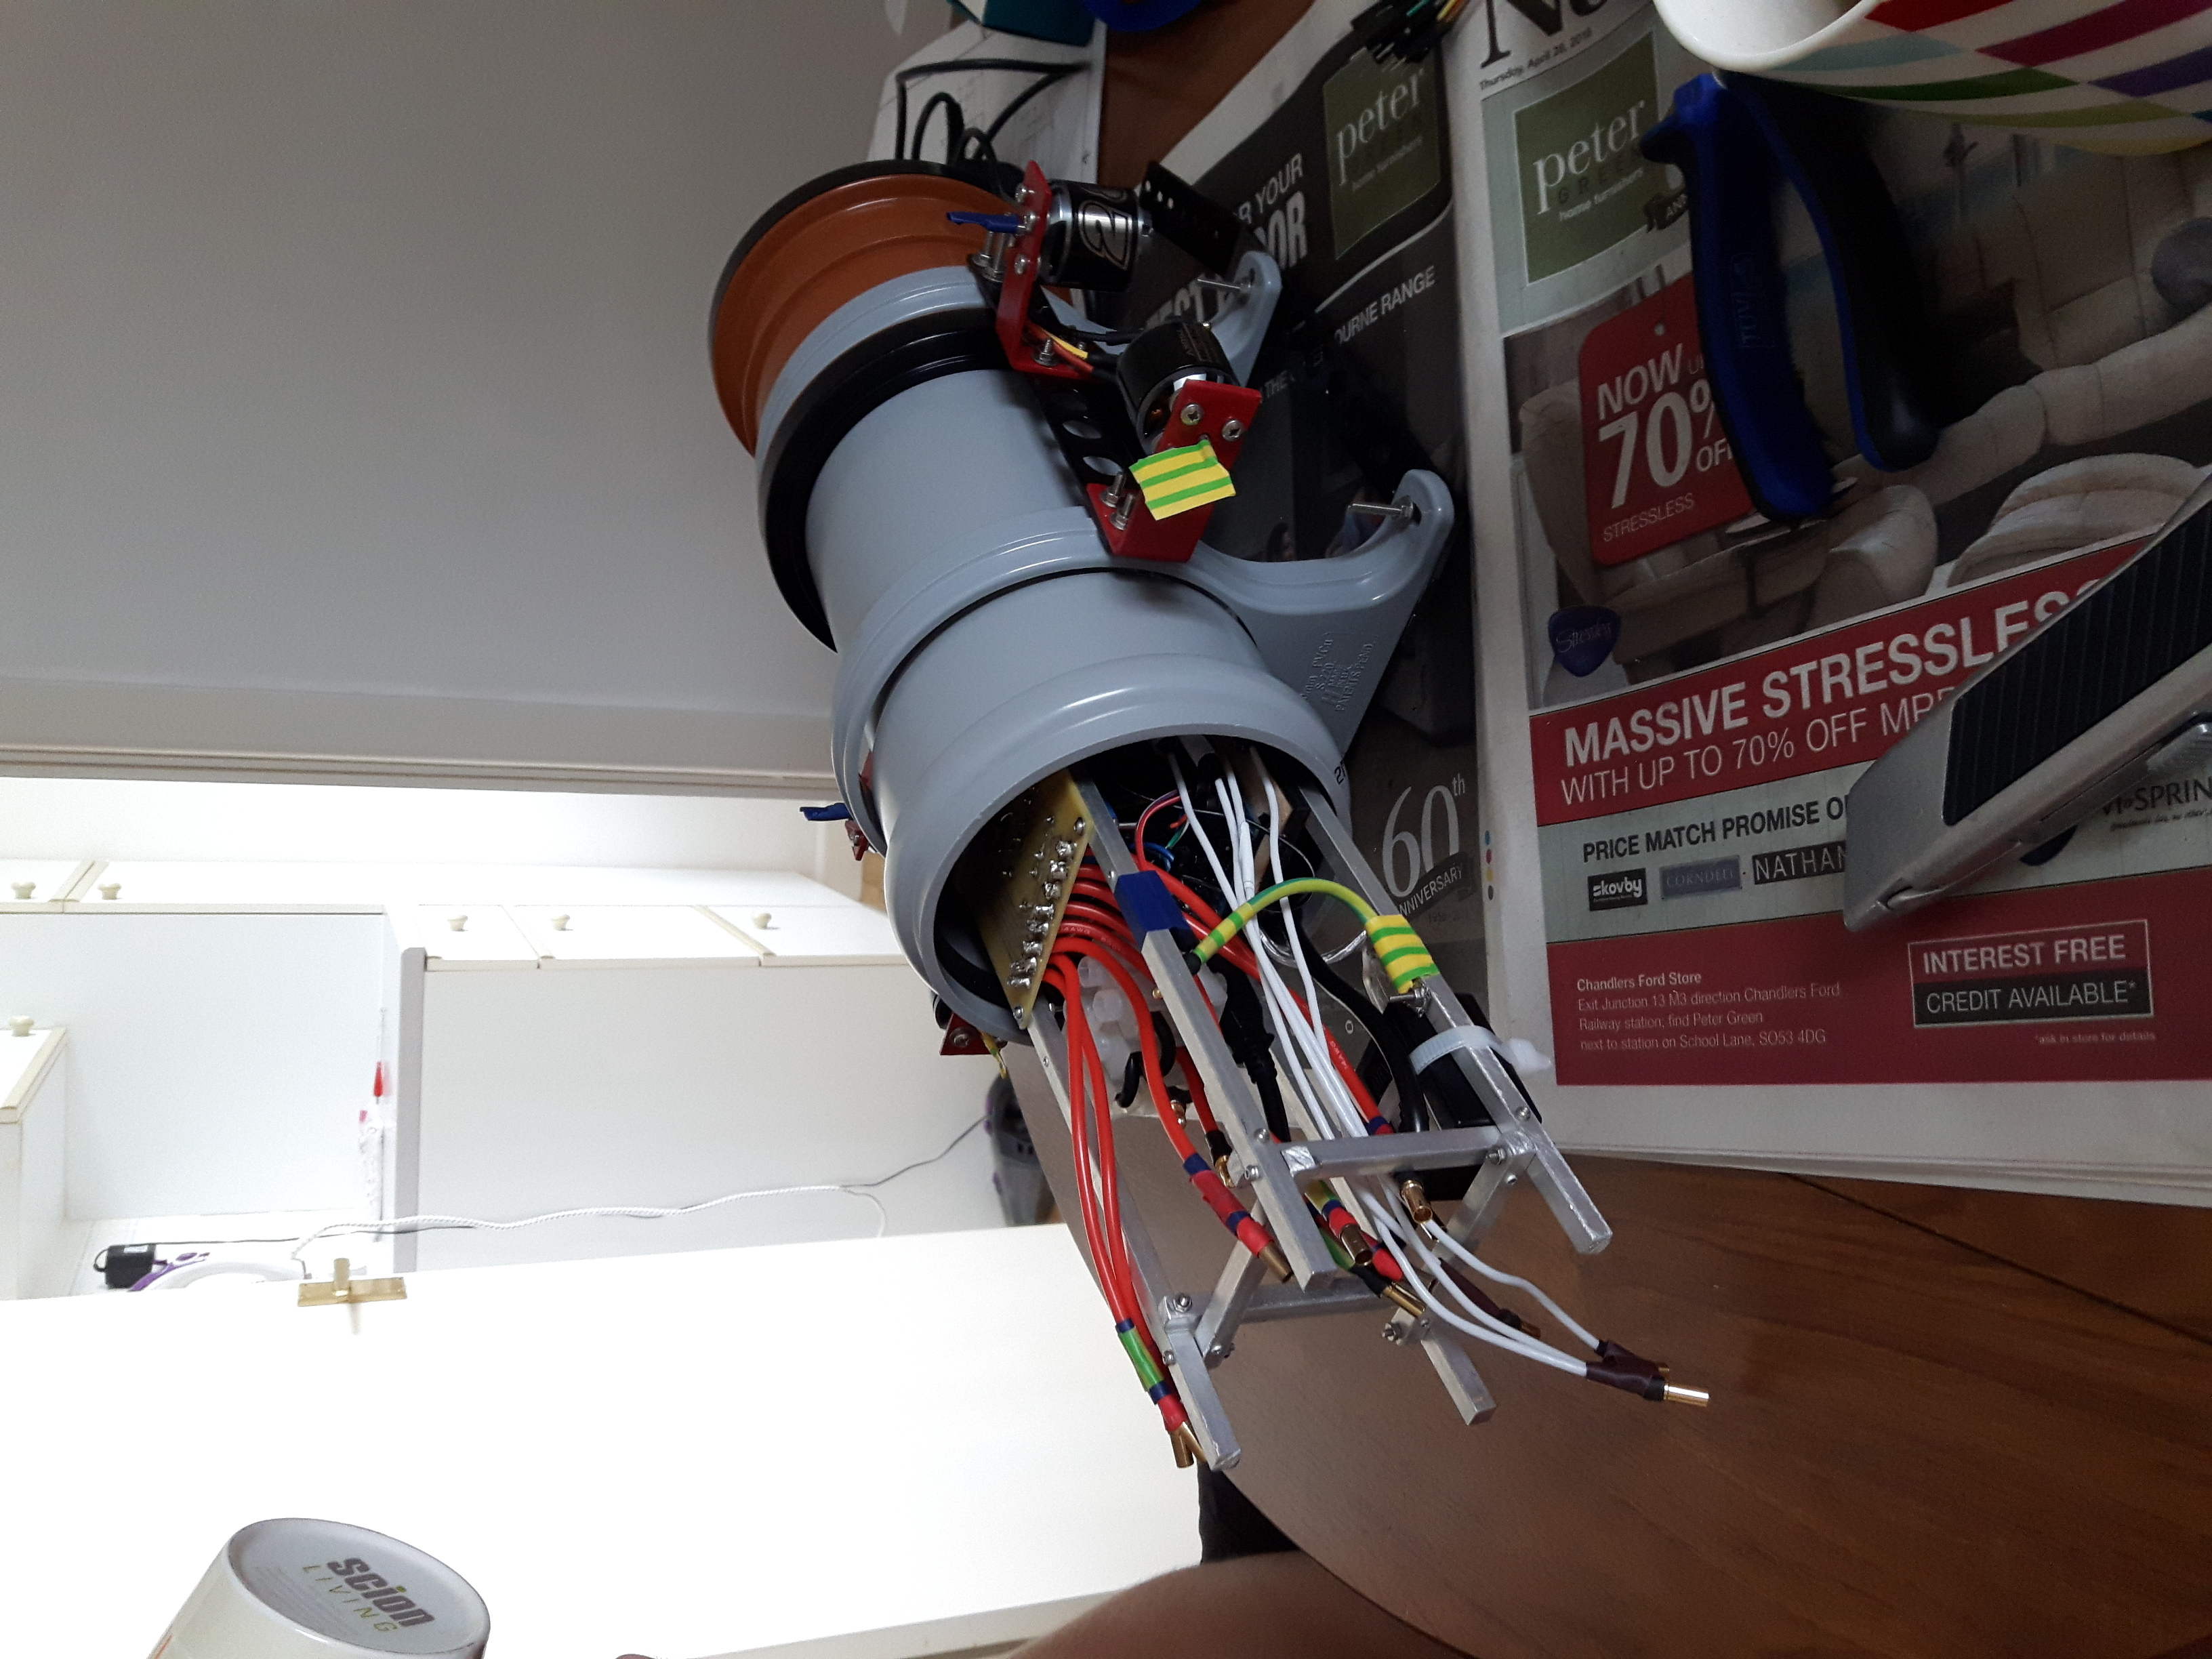
\includegraphics[width=\linewidth,angle=270]{20160625_145830.jpg}
\end{minipage}
\caption{Electronics are mounted to the internal aluminium structure, which slides into the pressure vessel.}
\label{fig:electronicsSlideIn}
\end{figure}

\begin{figure}[htb]
\begin{minipage}[b]{1\linewidth}
  \centering
	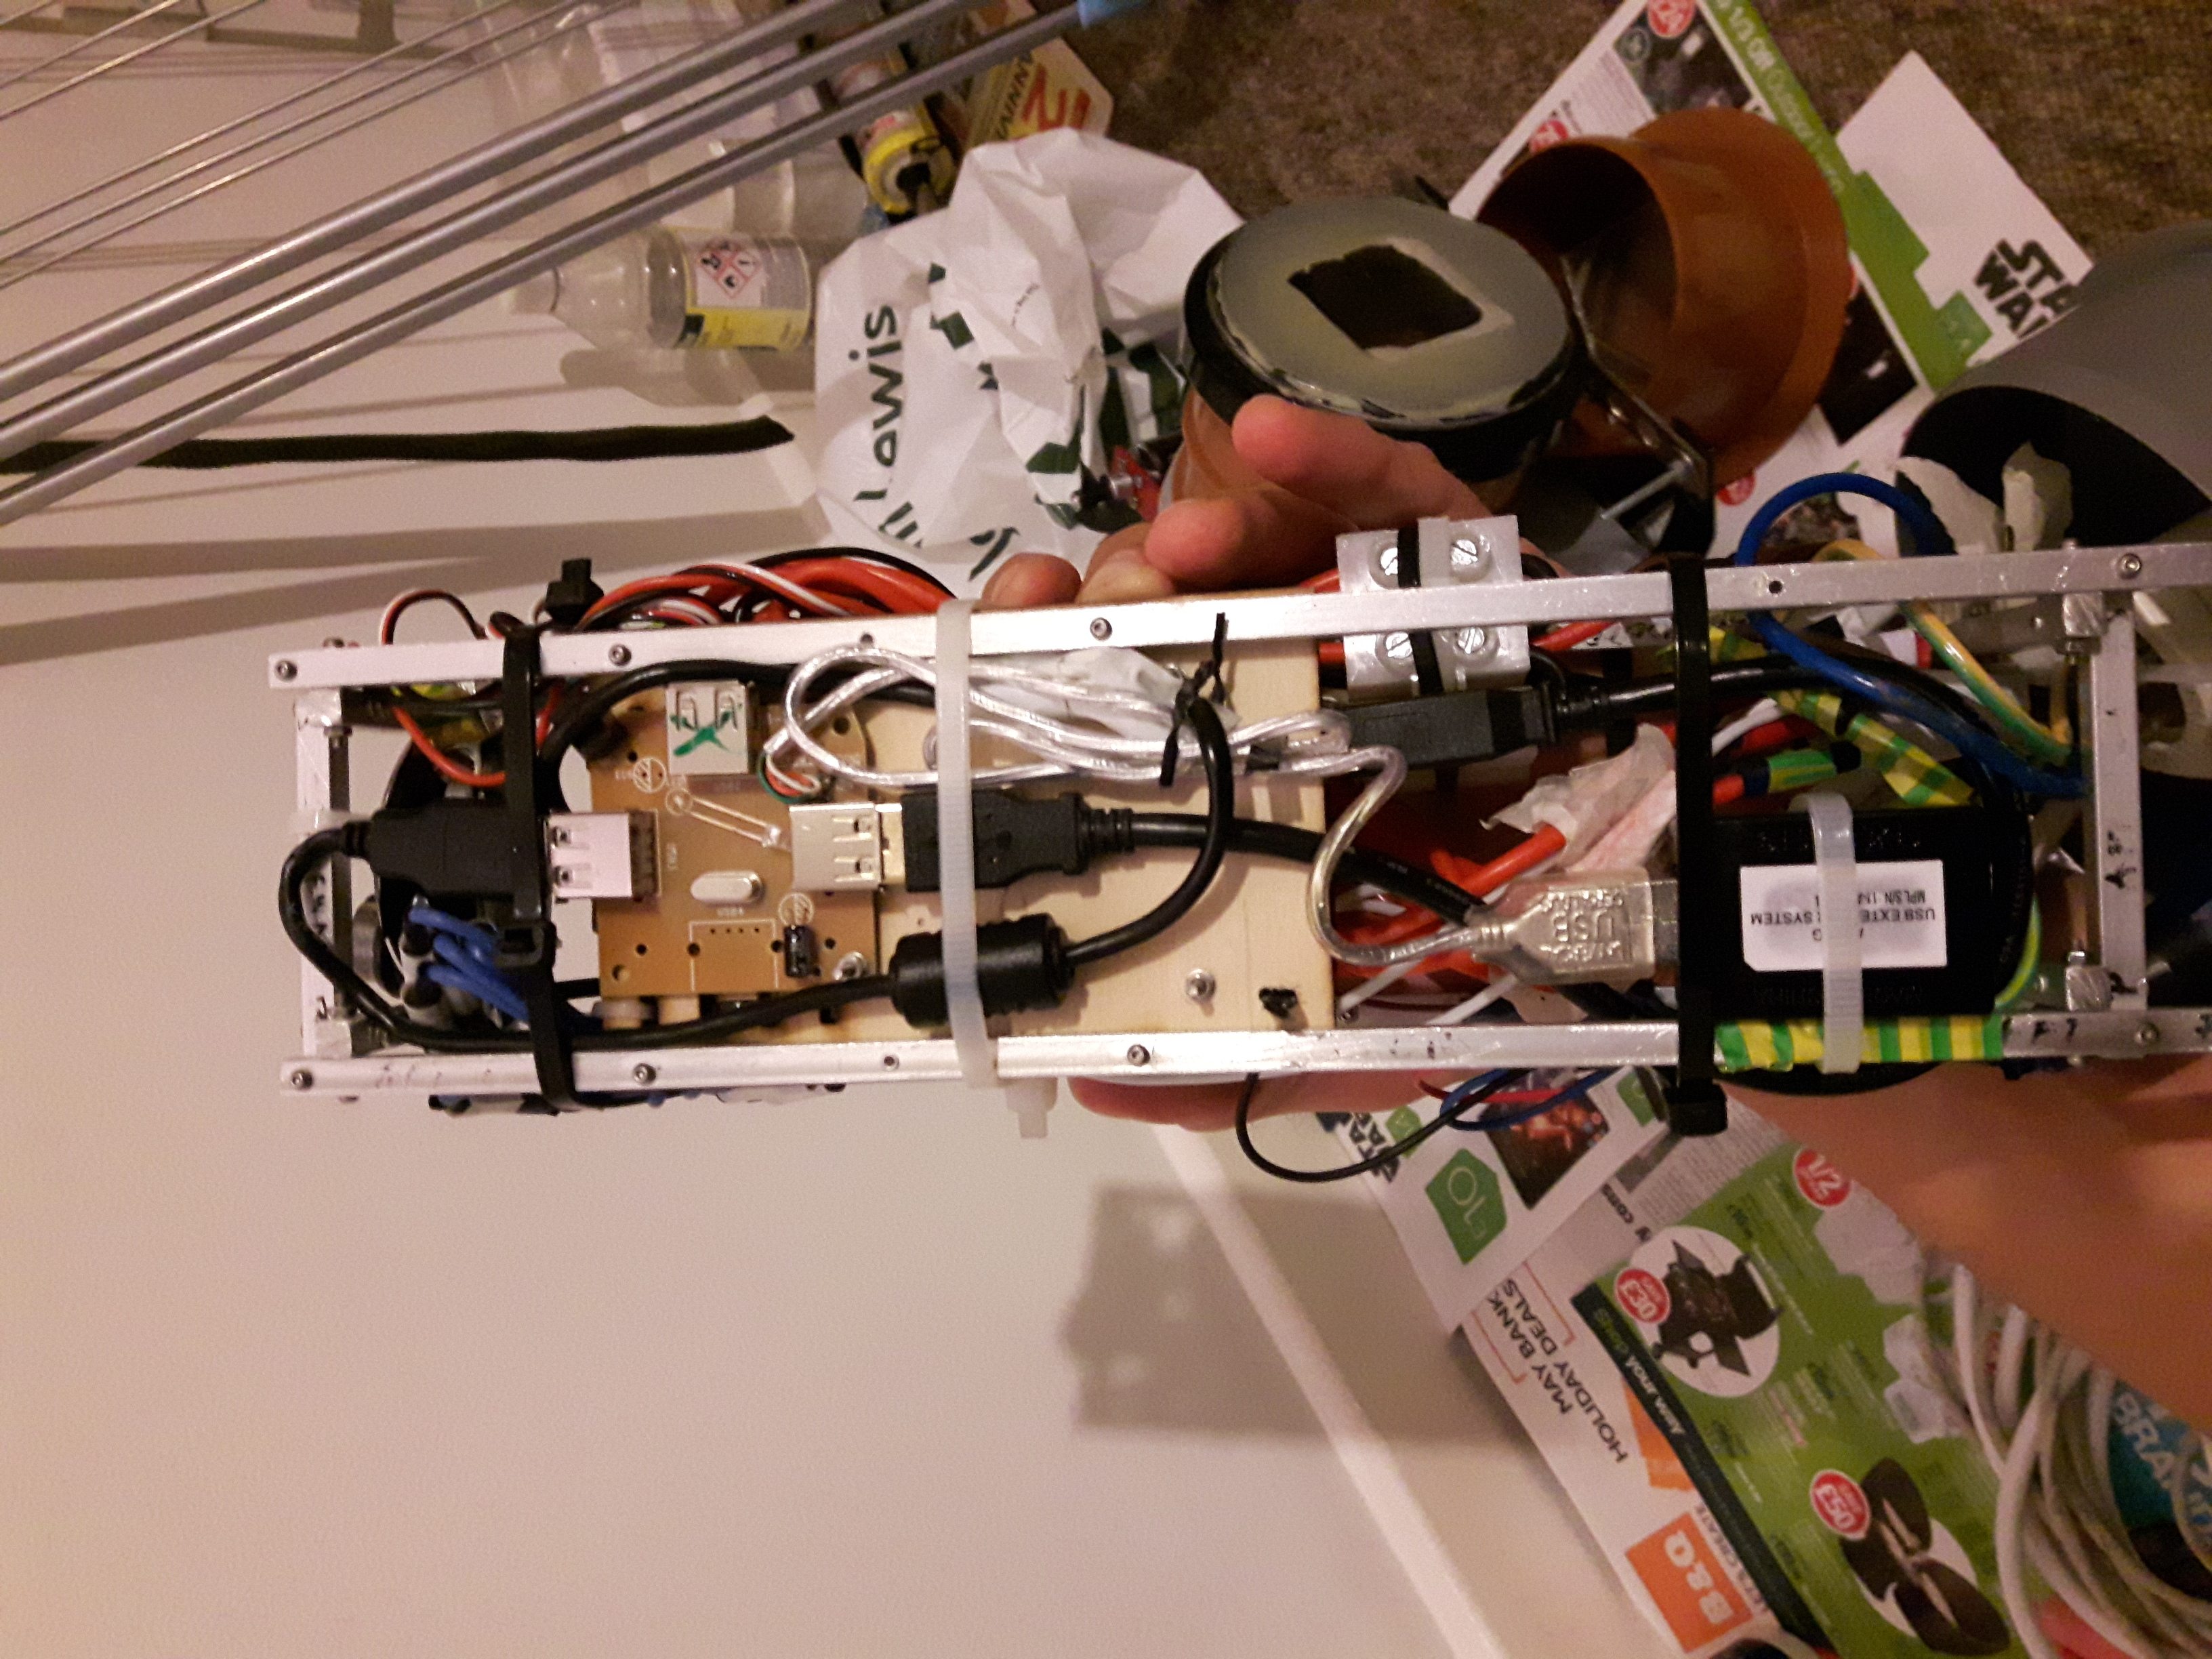
\includegraphics[width=\linewidth,angle=270]{20160826_213537.jpg}
\end{minipage}
\caption{USB range extender (black box on the bottom left of the phot) is mounted to the aluminium internal structure with a~white cable tie. The USB hub, into which Arduino and the webcam are plugged in, is bolted onto the underside of the plywood bed.}
\label{fig:usbExtenderAndHub}
\end{figure}

\begin{figure}[htb]
\begin{minipage}[b]{1\linewidth}
  \centering
	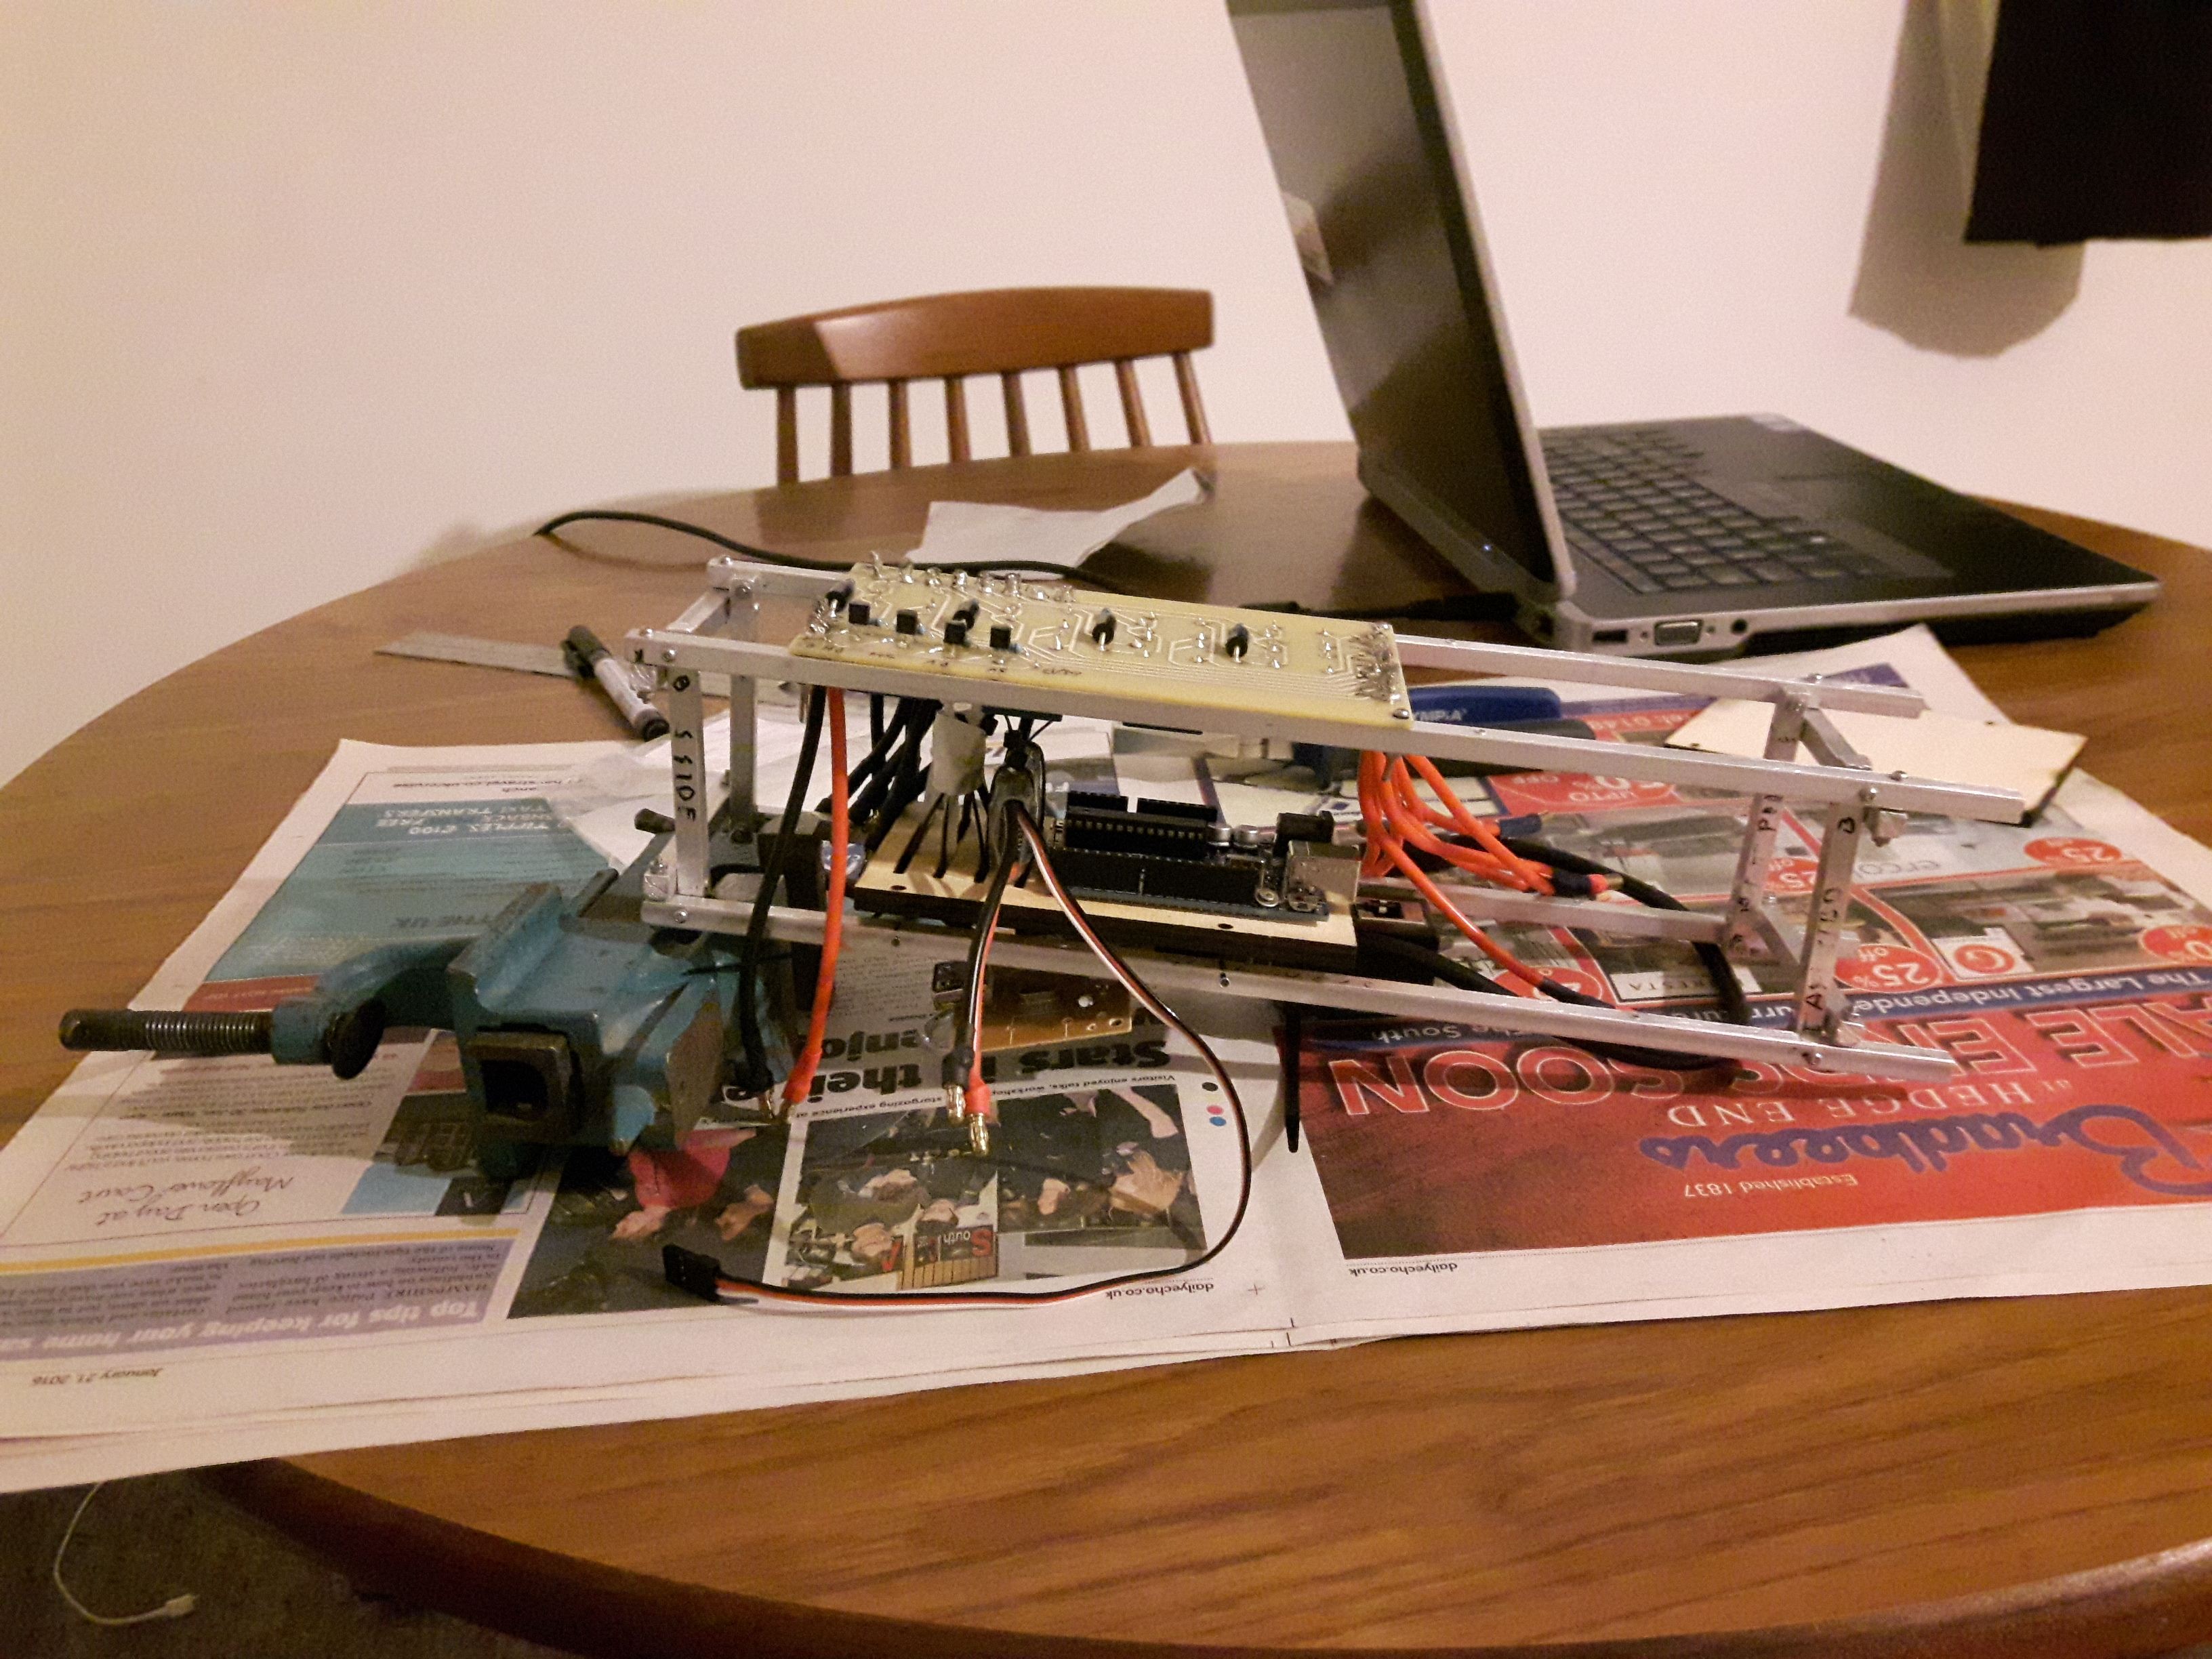
\includegraphics[width=\linewidth]{20160518_223426.jpg}
\end{minipage}
\caption{General arrangement of the internal electronics. Only one electronic speed controller, and no LEDs and camera are mounted for clarity.}
\label{fig:simpleInternalOverview}
\end{figure}

\clearpage % Place these figures close to the text.

%-------------------------------------------------------------------------------
\subsection{Power distribution subsystem}\label{ssection:powerDsitrbution}
Block diagram of the on-board power distribution subsystem is shown in Fig.~\ref{fig:powerBlockDiagram}. The Arduino and the camera are powered directly from the USB bus delivered on board via the CAT5 cable, which forms part of the tether (c.f. section~\ref{section:umbilical}). The USB bus is changed from the CAT5 cable to a~standard USB cable using the USB range extender, and then split by the USB hub to deliver power to both the camera and the Arduino.

The pressure sensor is powered from the Arduino \unit[5]{V} pin. The LEDs are turned on by setting an Arduino pin high, which provides sufficient power for them to operate. Both the pressure sensor and the LEDs are connected to the Arduino ground, and connections to both peripherals are realised using hookup wires.

The power for the ESCs and the motor control board is delivered from the shore-based battery via the power cable, which constitutes part of the tether. Custom power distribution unit (PDU) and common ground for these five components were manufactured out of automotive cable connectors. These components are shown in Fig.~\ref{fig:commonGround}; they connect the ESCs and the motor control board in parallel.

The ground (GND) of the Arduino is connected to four ESCs. However, these connections are separate from the ones that deliver power to the ESCs (negative battery terminals). Whether the Arduino GND and and battery GND are connected via the ESCs is unknown. The motor control board connects the Arduino and battery GND, as described in section~\ref{ssection:motorControlBoard}.

Power is delivered to the ESCs and motor control board using gauge 32 wires (thick lines in Fig.~\ref{fig:powerBlockDiagram}). All other connections in Fig.~\ref{fig:powerBlockDiagram} are realised using hookup wires.

The third wire in the power cable (besides battery positive and negative terminals) is used to ground the internal structure. This is intended to protect the operators in case the battery positive terminal short-circuits to one of the internal components or the aluminium structure. The external structure is not grounded.

The shore battery pack constitutes two \unit[6]{V} batteries connected in series. These are housed inside an aluminium box, which also incorporates a~\unit[20]{mm} fuse, switches and leads that can be used to monitor the battery voltage. Disassembled battery pack is shown in Fig.~\ref{fig:batteryPack}.

\begin{figure}[htb]
\begin{minipage}[b]{1\linewidth}
  \centering
	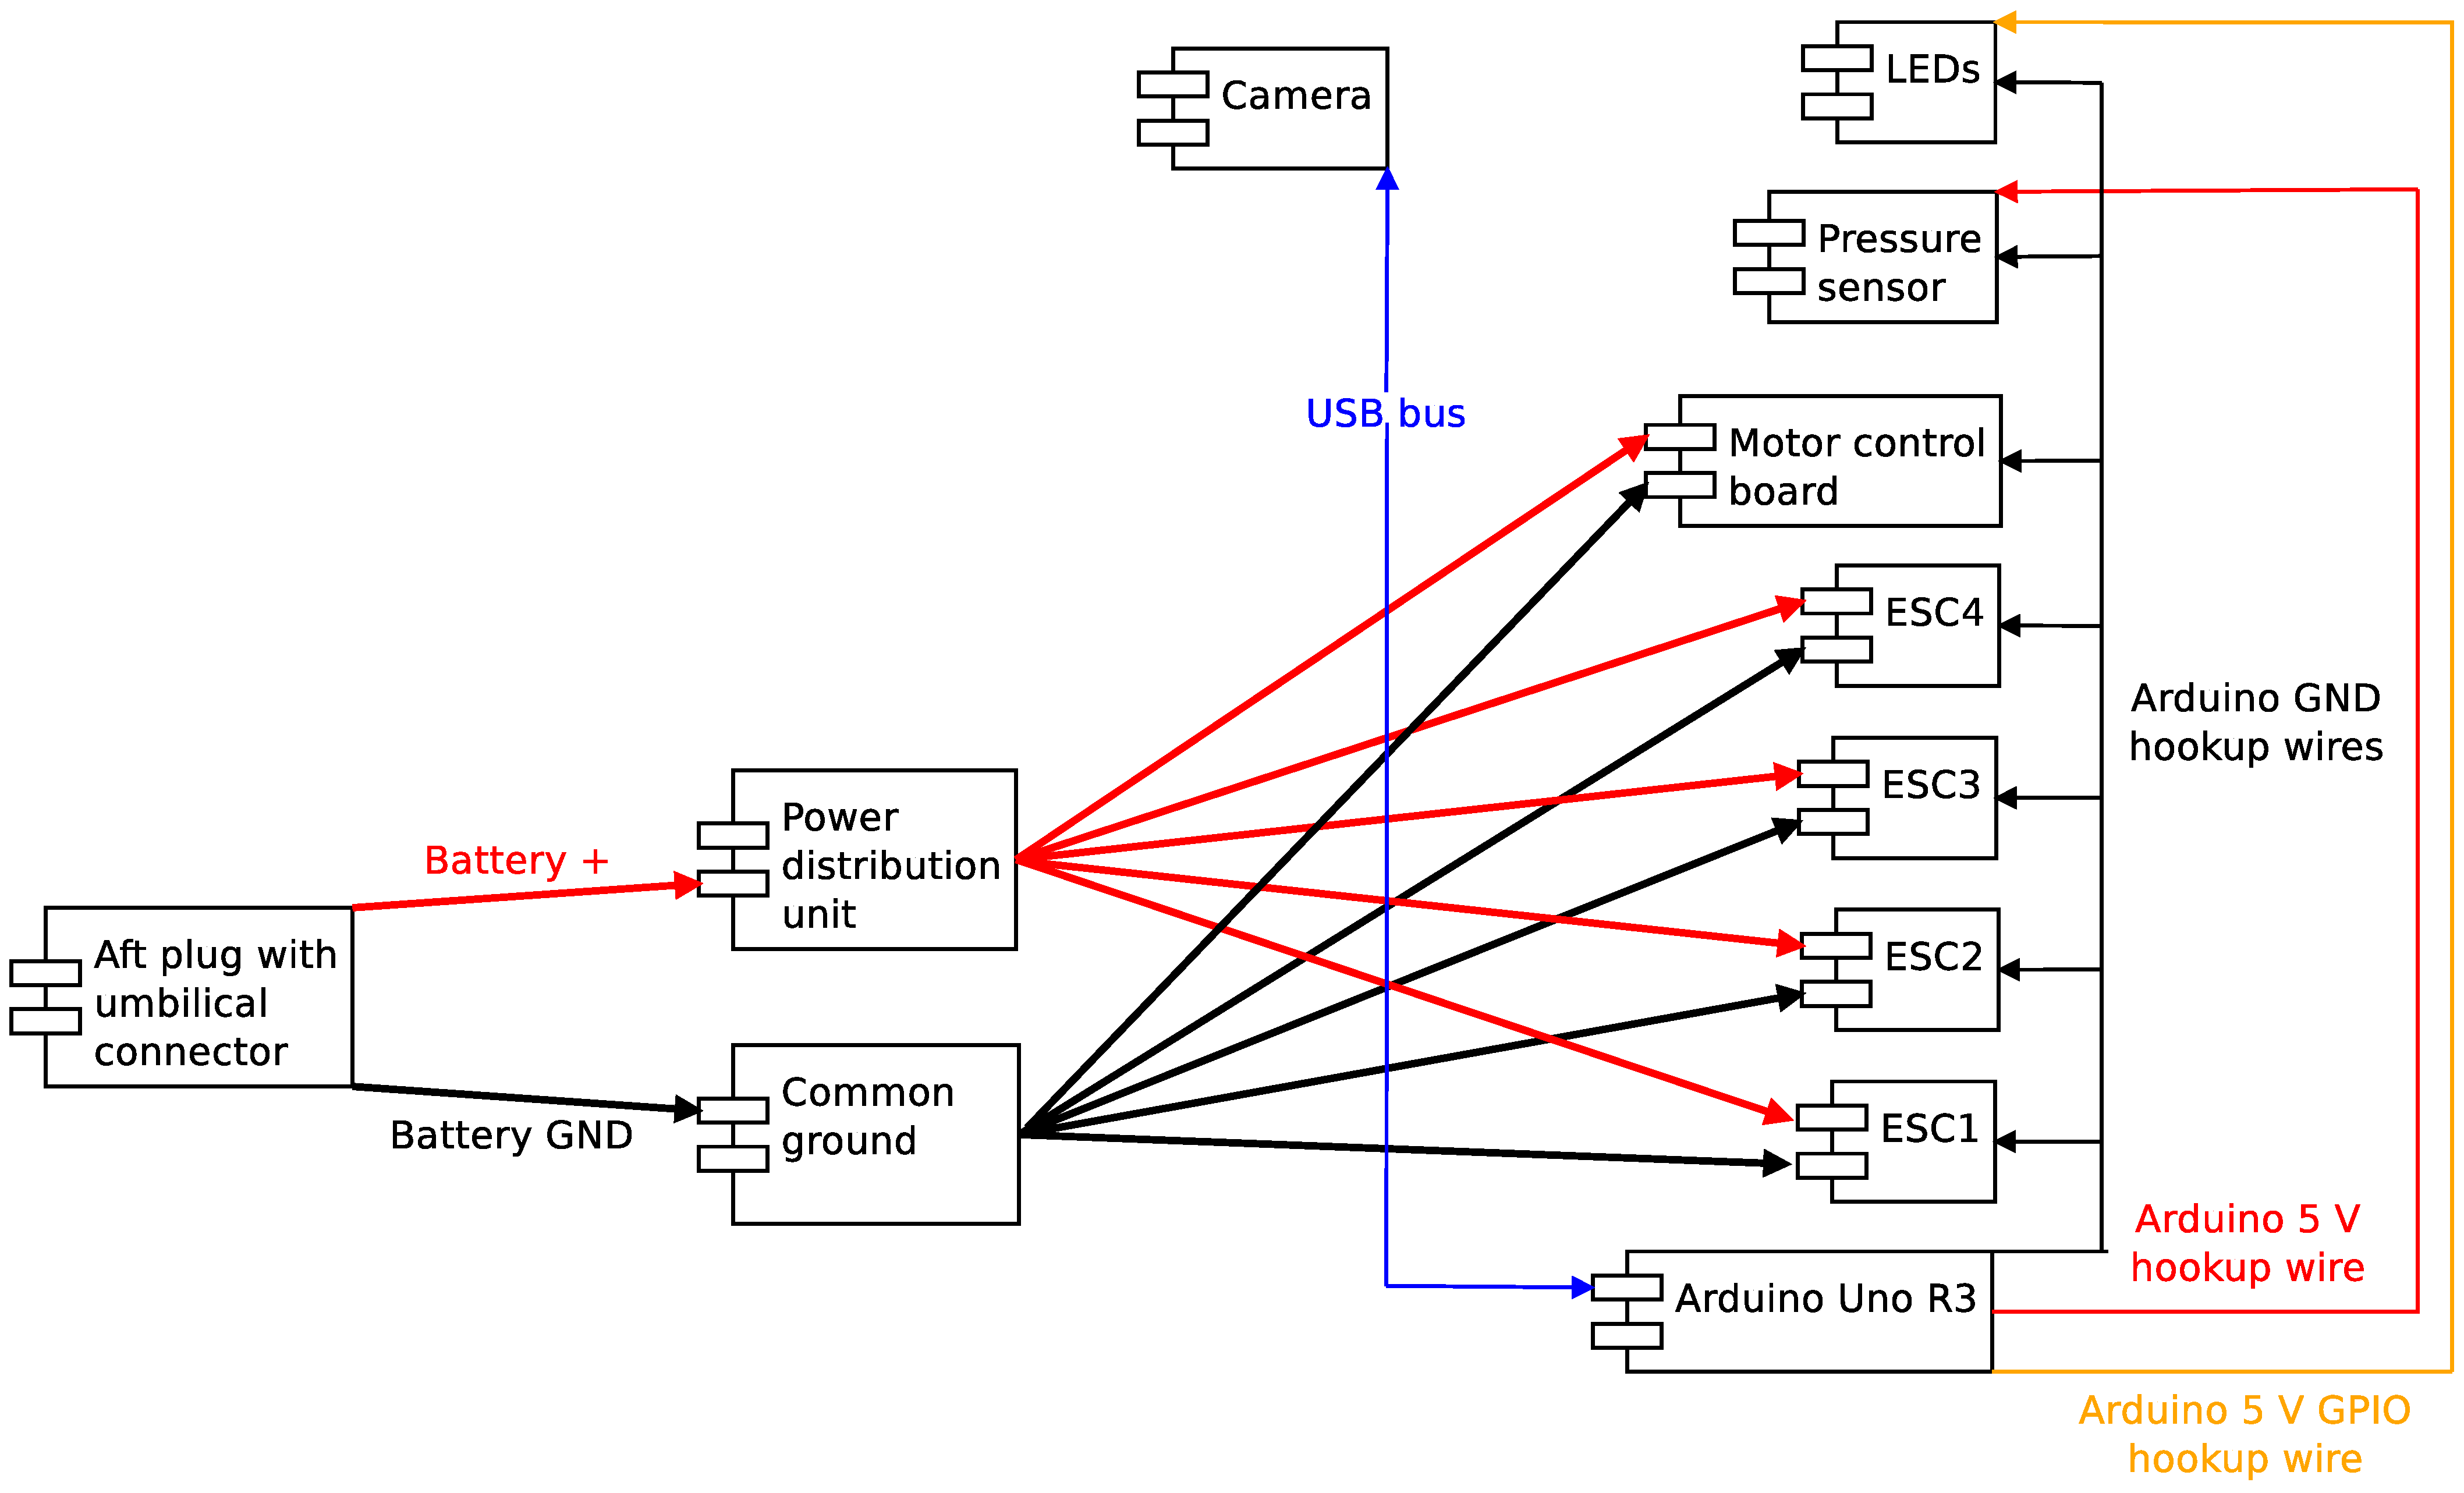
\includegraphics[width=1\linewidth,angle=90]{powerBlockDiagram.eps}
\end{minipage}
\caption{Block diagram of the power distribution subsystem. Power is delivered to the aft plug using the umbilical tether, which is connected to the battery pack.}
\label{fig:powerBlockDiagram}
\end{figure}

\begin{figure}[htb]
\begin{center}
\begin{tabular}{c c}
	\subfloat[Side]
		{\includegraphics*[width=0.6\textwidth,angle=270]{20160826_213345.jpg}
		\label{fig:commonGround:label:a} } &
	\subfloat[Top]
		{\includegraphics*[width=0.6\textwidth,angle=270]{20160826_213835.jpg}
		\label{fig:commonGround:label:b} } \\
\end{tabular}
\end{center}
\caption{Side and top views of the common ground and common power lines made out of screw automotive cable connectors and mounted to the aluminium internal structure with cable ties.}
\label{fig:commonGround}
\end{figure}

\begin{figure}[htb]
\begin{minipage}[b]{1\linewidth}
  \centering
	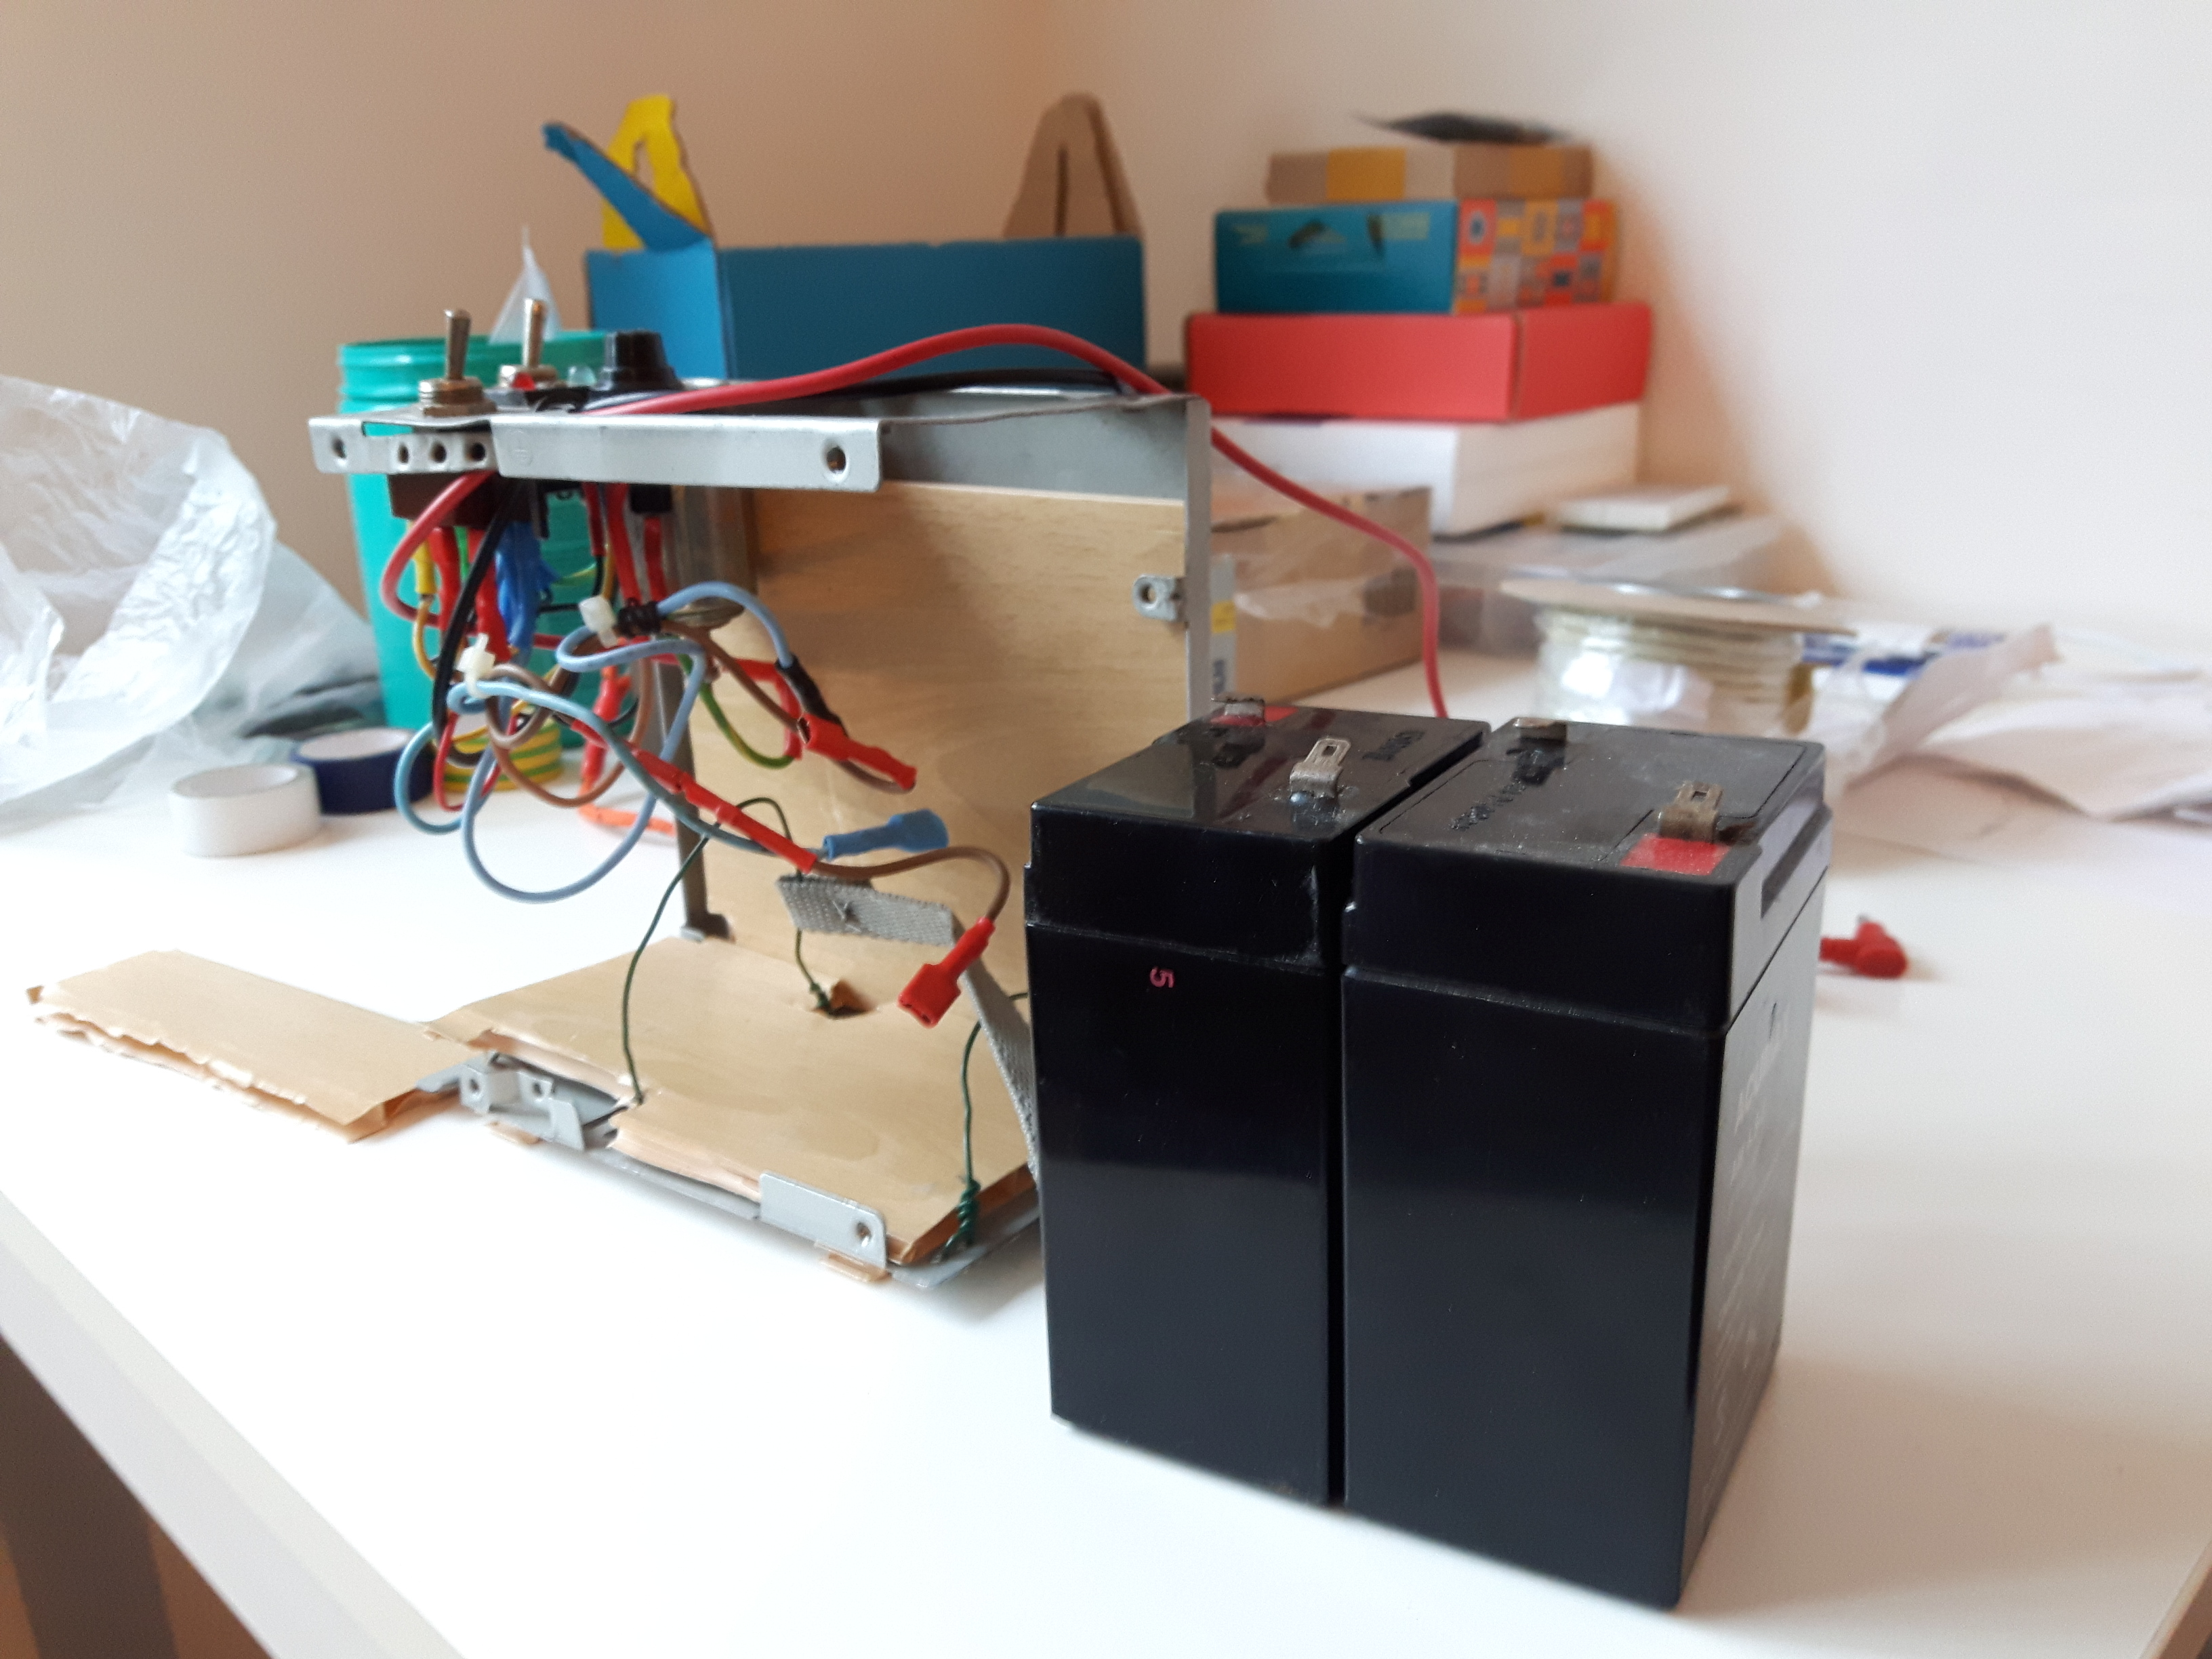
\includegraphics[width=1\linewidth]{20160828_184532.jpg}
\end{minipage}
\caption{Disassembled battery pack. One switch enables the batteries to be connected in parallel or in series (series configuration is used for the ROV project) while the other one switches the power on or off. The output of the battery pack is protected from excessive currents using a~\unit[20]{mm} fuse.}
\label{fig:batteryPack}
\end{figure}

\clearpage % Place these figures close to the text.

%-------------------------------------------------------------------------------
\subsection{Propulsion subsystem}\label{ssection:propulsionSubsystem}
Block diagram of the ROV propulsion subsystem is shown in Fig.~\ref{fig:propulsionBlockDiagram}. It is based on four brushless DC motors that are driven by four commercial, off-the-shelf electronic speed controllers. Every ESC converts a~pulse width modulation signal (PWM) from the Arduino into pulses of power delivered to every of three terminals on the brushless motor. Changing the frequency of the PWM changes the frequency of the power pulses, which changes the rotation frequency of the motor and so also its thrust. This PWM signal is delivered from the Arduino pins using hookup wires. The ESCs draw power, which is then delivered to the motors in pulses, directly from the shore-based batteries, which is described in section~\ref{ssection:powerDsitrbution}.

In order to reverse thrust of the motor, it suffices to swap two out of three signals output by the ESC. This is achieved by a~custom printed circuit board, which is described in more detail in section~\ref{ssection:motorControlBoard}. Two out of three outputs of every ESC (terminals 1 and 2 in Fig.~\ref{fig:propulsionBlockDiagram}) are routed through this board, before they are delivered to the corresponding motors using the connector in the aft plug using red wires in Fig.~\ref{fig:electronicsSlideIn}. The third signal of every ESC (terminal 3 in Fig.~\ref{fig:propulsionBlockDiagram}) circumvents the motor control board and connects to the corresponding motor only through the connector in the aft plug (white wires in Fig.~\ref{fig:electronicsSlideIn}). The commands to swap the thrust of a~given motor are issued to the motor control board via hookup wires connected to the Arduino pins.

The ESCs are mounted to the plywood bed ahead of the Arduino using cable ties (the aft-most ESC is visible in Fig.~\ref{fig:simpleInternalOverview}). The ESCs connect to the motor control board, the aft plug connector, and the motors using gauge 32 wires.

\begin{figure}[htb]
\begin{minipage}[b]{1\linewidth}
  \centering
	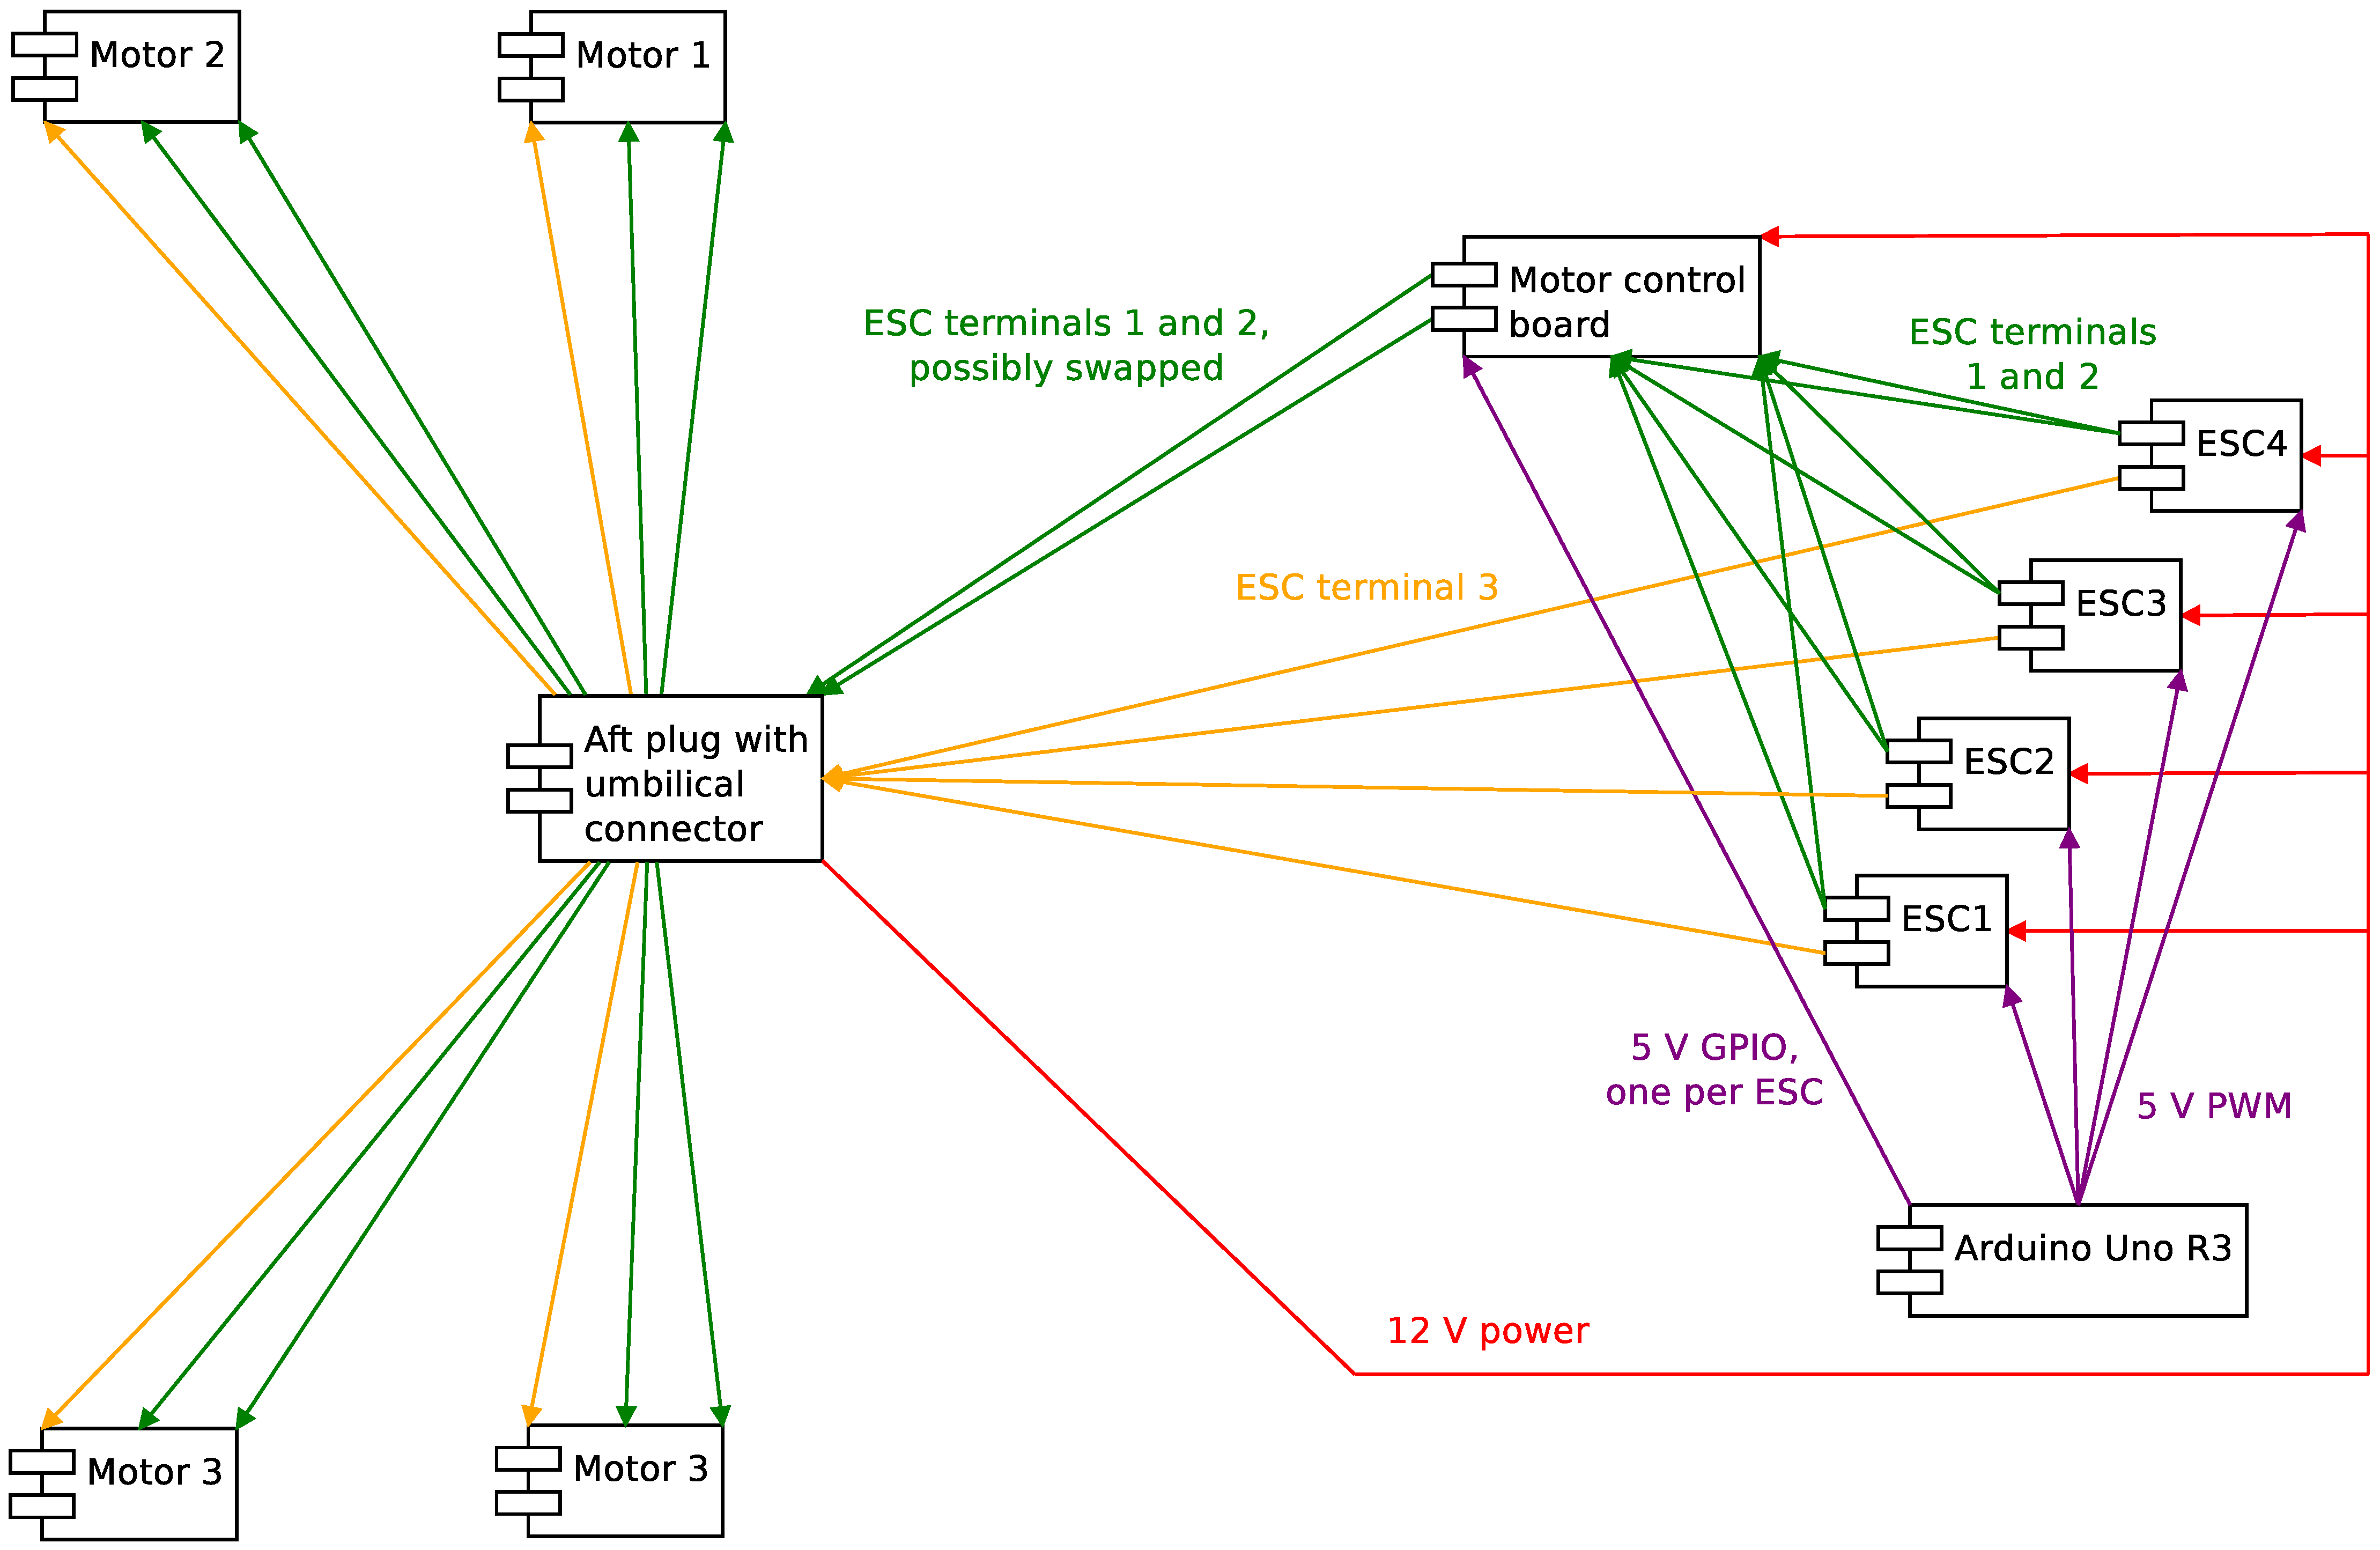
\includegraphics[width=1\linewidth,angle=90]{propulsionBlockDiagram.eps}
\end{minipage}
\caption{Block diagram of the ROV propulsion subsystem. \textcolor{purple}{Connections from the Arduino} are realised using hookup wires. All other signals (\textcolor{red}{power}, and ESC signals \textcolor{green}{1, 2} and \textcolor{orange}{3}) are carried using gauge 32 wire.}
\label{fig:propulsionBlockDiagram}
\end{figure}

%-------------------------------------------------------------------------------
\subsection{Brushless-motor control board}\label{ssection:motorControlBoard}
As explained in section~\ref{ssection:propulsionSubsystem}, two signals from every ESC have to be swapped in order to reverse the thrust of a~motor. The schematic of the circuit, which achieves this, is shown in Fig.~\ref{fig:motorControlBoardSchematic}. Nominally, terminals 1 and 2 of every ESC (e.g. ESC1T1 and ESC1T2 for ESC no.~1) are connected to terminals 1 and 2 of the corresponding motor (e.g. M1T1 and M1T2 for motor no.~1). When a~command to reverse the thrust of a~given motor is issued by the Arduino by setting one of its pins high (e.g. pin~2 for motor no.~1), an n-type mosfet activates two switching relays. This connects terminals 1 and 2 of the ESC with terminals 2 and 1 of the motor, respectively, thus reversing the thrust. When the command pin is set low, the relays switch back to the nominal configuration and thrust is no longer reversed.

The power output of the Arduino is insufficient to activate the relays - relatively large relays, which can withstand currents output by the ESCs, have to be used. Thus, the power to the relays is delivered by the shore-based batteries. Every ESC-motor pair requires two switching relays, and every two relays have one flyback diode.

A~two-layer PCB houses the entire circuit from Fig.~\ref{fig:motorControlBoardSchematic}; its layout is shown in Fig.~\ref{fig:motorControlBoardLayout}. The motor control PCB is manufactured with 1 oz Cu and has trace widths of at least \unit[1]{mm} rated to at least \unit[2.5]{A}. The design of this board is open-source, and can be accessed in its repository at: \textcolor{blue}{\url{{www.upverter.com/AleksanderLidtke/7eccd1441d1097f8/BrushlessMotorControlBoard/}}}.

\begin{figure}[htb]
\begin{minipage}[b]{1\linewidth}
  \centering
	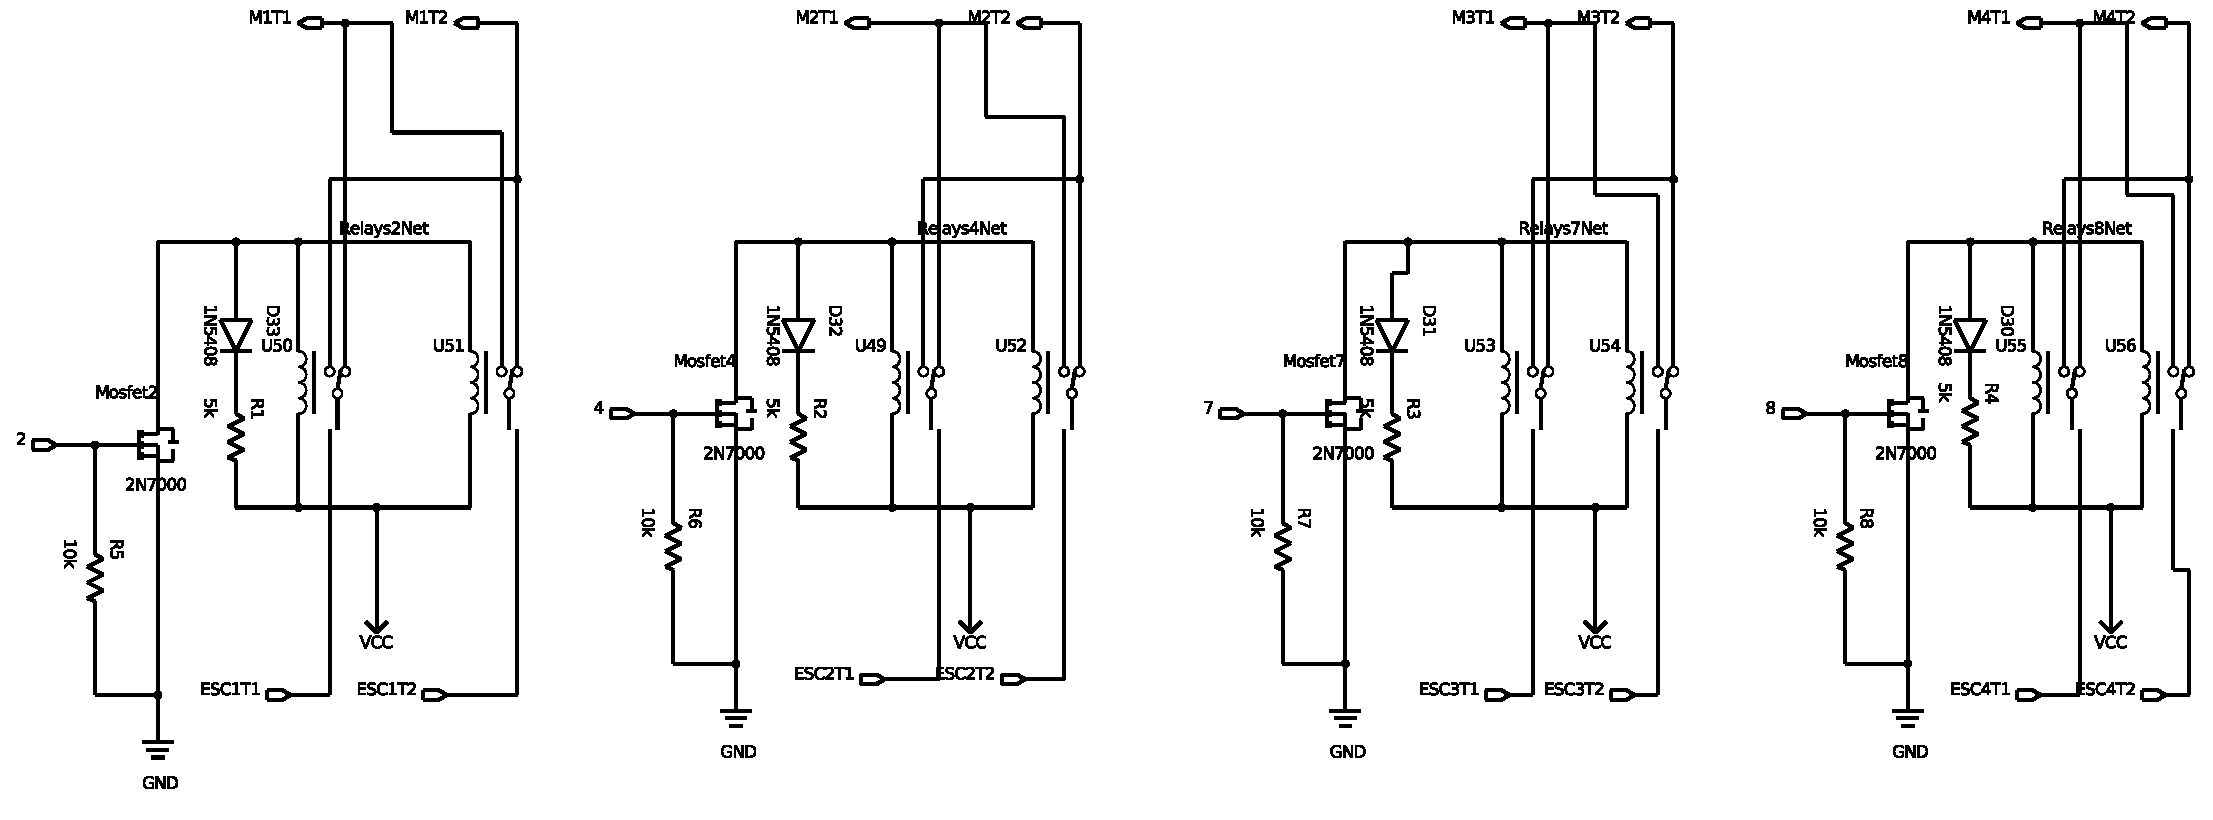
\includegraphics[width=1\linewidth,angle=90]{motorControlBoardSchematic.pdf}
\end{minipage}
\caption{Schematic of the brushless motor control PCB. The board connects terminals of ESCs to motor terminals via pairs of switching relays.}
\label{fig:motorControlBoardSchematic}
\end{figure}

\begin{figure}[htb]
\begin{minipage}[b]{1\linewidth}
  \centering
	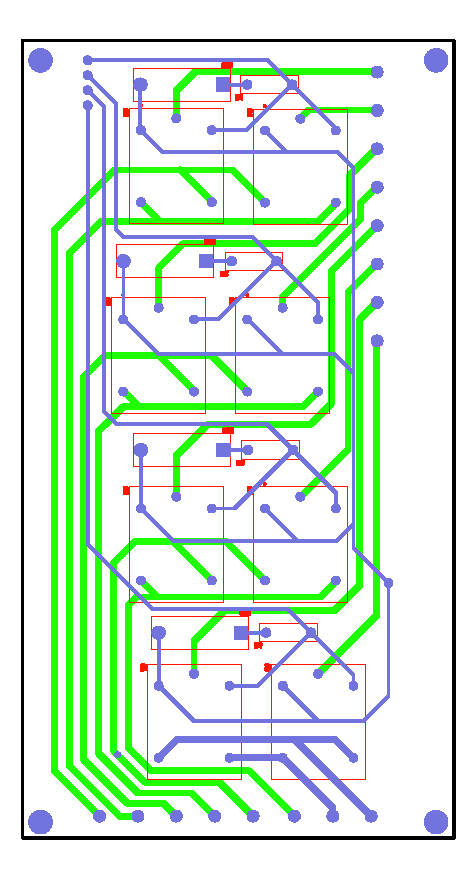
\includegraphics[width=0.75\linewidth]{motorControlBoardLayout.eps}
\end{minipage}
\caption{Layout of the brushless motor control PCB. Bottom copper marked with \textcolor{green}{green}, top with \textcolor{blue}{blue}, and component outlines with \textcolor{red}{red}. Switching relays are mounted on the top, and resistors, diodes and n-type mosfets on the bottom of the board. The PCB is actually mounted upside down in the vehicle, so that the bottom copper layer is facing the top of the ROV.}
\label{fig:motorControlBoardLayout}
\end{figure}

\clearpage % Place these figures close to the text.

%-------------------------------------------------------------------------------
\subsection{LEDs and camera}\label{ssection:ledAndCamera}
A~small, one-layer PCB, which houses three white LEDs connected in series, is mounted to a~reflective plastic surface. A~hole is drilled in the plastic, through which a~disassembled USB webcam is pointed in the direction of the LED lights. These LEDs and camera form a~stand-alone module, which is shown in Fig.~\ref{fig:forwardLED:label:a}. The module is mounted to the front of the internal aluminium frame of the ROV using cable ties, as shown in Fig.~\ref{fig:forwardLED:label:b}. A~translucent window is placed in the pressure vessel in front of the camera, which is described in section~\ref{ssection:forwardPlug}. As shown in Fig.~\ref{fig:powerBlockDiagram}, the LEDs are activated and powered directly from a~GPIO pin of the Arduino, whereas the camera is powered and operated via the USB bus.

\begin{figure}[htb]
\begin{center}
\begin{tabular}{c c}
	\subfloat[LED and camera module]
		{\includegraphics*[width=0.6\textwidth,angle=270]{20160319_174439.jpg}
		\label{fig:forwardLED:label:a} } &
	\subfloat[Module mounting]
		{\includegraphics*[width=0.6\textwidth,angle=270]{20160826_213436.jpg}
		\label{fig:forwardLED:label:b} } \\
\end{tabular}
\end{center}
\caption{The module, which houses the LEDs and the camera, and its mounting in the vehicle.}
\label{fig:forwardLED}
\end{figure}

%-------------------------------------------------------------------------------
\subsection{Pressure sensor}\label{ssection:pressureSensor}

A~\unit[30]{PSI} pressure transducer, depicted in Figure \ref{fig:pressureTransducer}, is mounted in the aft plug, which is a~modified PVC socket plug shown in Fig.~\ref{fig:socketPlug}. A~hole was punched in the socket plug, into which the pressure sensor was screwed in. The connection was sealed by applying PTFE tape on the thread of the pressure transducer and inserting rubber washers on either side of the socket plug. The entire assembly was then tightened using a~nut and a~washer placed on the external side of the socket plug. The inlet of the pressure sensor, brass nut and a~steel washer, under which a~rubber washer is placed, can be seen in Fig.~\ref{fig:externalSideOfTheAftPlug}. The transducer is powered from the Arduino \unit[5]{V} pin through a~hookup wire. It is connected to the Arduino GND and an analogue input pin using hookup wires as well.

\begin{figure}[htb]
\centering
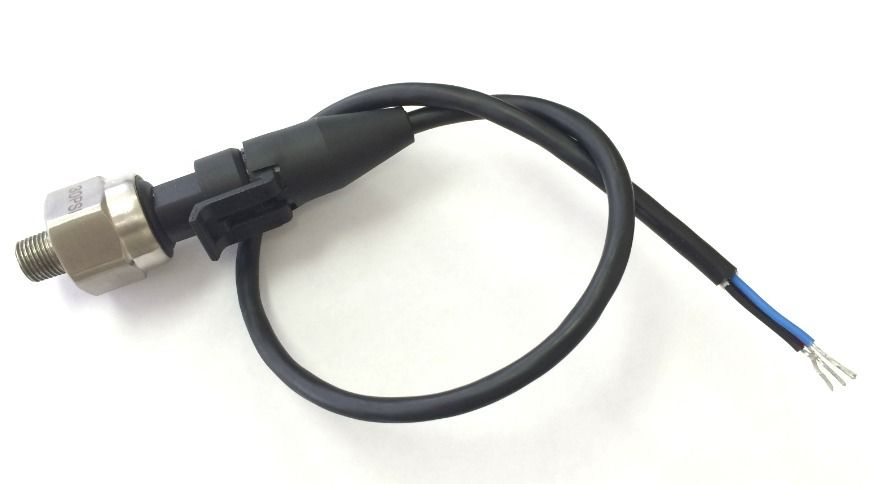
\includegraphics[width=0.8\linewidth]{pressureTransducer.jpg}
\caption{Overview of the pressure transducer.}
\label{fig:pressureTransducer}
\end{figure}

\begin{figure}[htb]
\begin{minipage}[b]{1\linewidth}
  \centering
	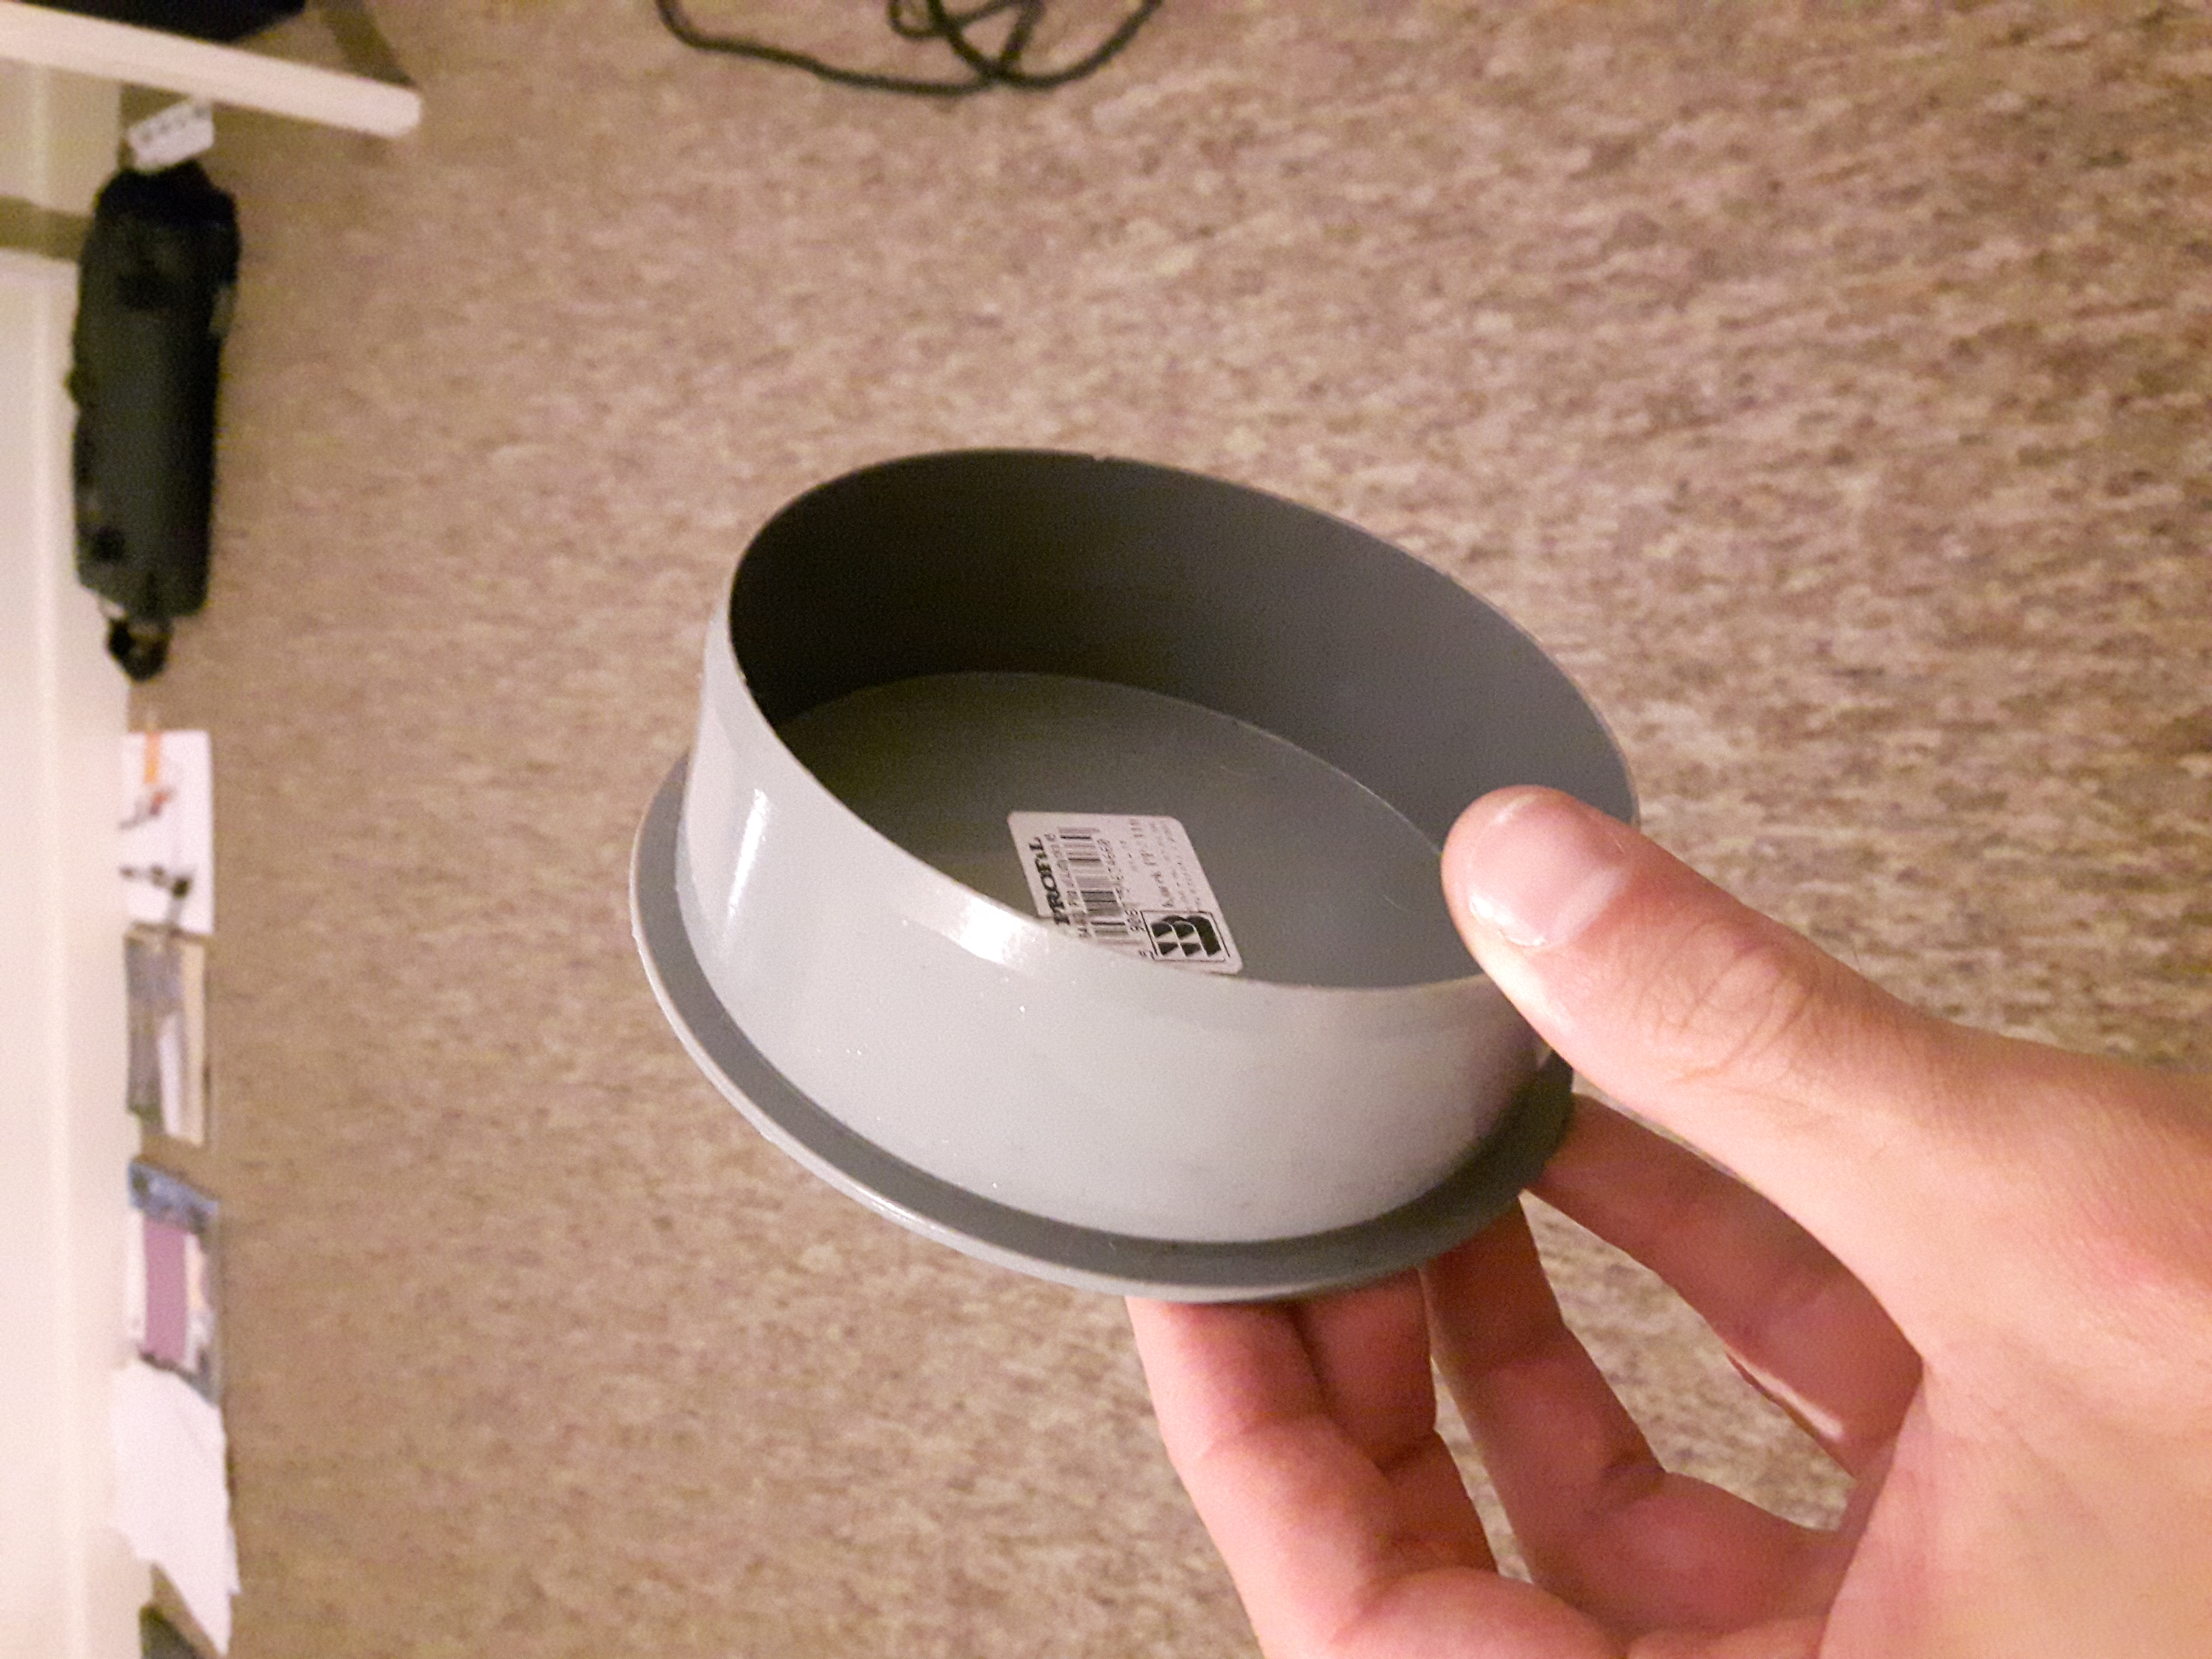
\includegraphics[width=\linewidth,angle=270]{20160826_213233.jpg}
\end{minipage}
\caption{Socket plug used to manufacture the aft and forward plug.}
\label{fig:socketPlug}
\end{figure}

%-------------------------------------------------------------------------------
\subsection{Ardunio pinout}\label{ssection:arduinoPinout}

Table \ref{tab:pinoutMain} describes all of the Arduino connections used by the ROV. Thrust direction pins are responsible for switching the relays on the motor control board via mosfet transistors, and throttle pins are connected to the ESCs directly and control motor rpm using PWM signals (see section~\ref{ssection:motorControlBoard} for details).

\begin{table}[h]
\centering
\caption{Pinout showing Arduino connections.}
\label{tab:pinoutMain}
\begin{tabular}{@{}ll@{}}
\toprule
\textbf{Pin  no.} & \textbf{Connect net} \\ \midrule
2 & Motor port horizontal - thrust direction \\
3 & Motor port horizontal - throttle \\
4 & Motor starboard horizontal - thrust direction \\
5 & Motor starboard horizontal - throttle \\
6 & Motor port vertical - throttle \\
7 & Motor port vertical - thrust direction \\
8 & Motor starboard vertical - thrust direction \\
9 & Motor starboard vertical - throttle \\
12 & Forward LED on/off \\
A0 & Pressure transducer analogue input \\
5 V & Pressure transducer VDD \\
\bottomrule
\end{tabular}
\end{table}

%===============================================================================
\section{Pressure vessel}\label{section:pressureVessel}

%-------------------------------------------------------------------------------
\subsection{Aft plug}\label{sscetion:aftPlug}
The aft plug is made of a~PVC socket plug shown in Fig.~\ref{fig:socketPlug}. Two holes were punched in it - one, into which the pressure transducer is screwed in, as described in section~\ref{ssection:pressureSensor}, and one, which houses the umbilical connector described in section~\ref{ssection:connectorOnTheROV}.

The external side of the aft plug (the wet side of the ROV), with the pressure transducer and umbilical connector mounted, is shown in Fig.~\ref{fig:externalSideOfTheAftPlug}. Its internal side is shown in Fig.~\ref{fig:internalSideOfTheAftPlug}; the body of the pressure sensor, CAT5 cable, power chord, and 12 motor wires (three signals per each of the four motors) can be seen on this side. The plug can be removed from the main pressure vessel to enable inspection and modification of the interior of the ROV. In order to ease the process and improve the water-tightness, silicone lubricant from Fig.~\ref{fig:lubricant} is applied on the aft plug before it is slid into the main pressure vessel. Once in place, the aft plug is secured using a~water-resistant duct tape.

\begin{figure}[htb]
\begin{minipage}[b]{1\linewidth}
  \centering
	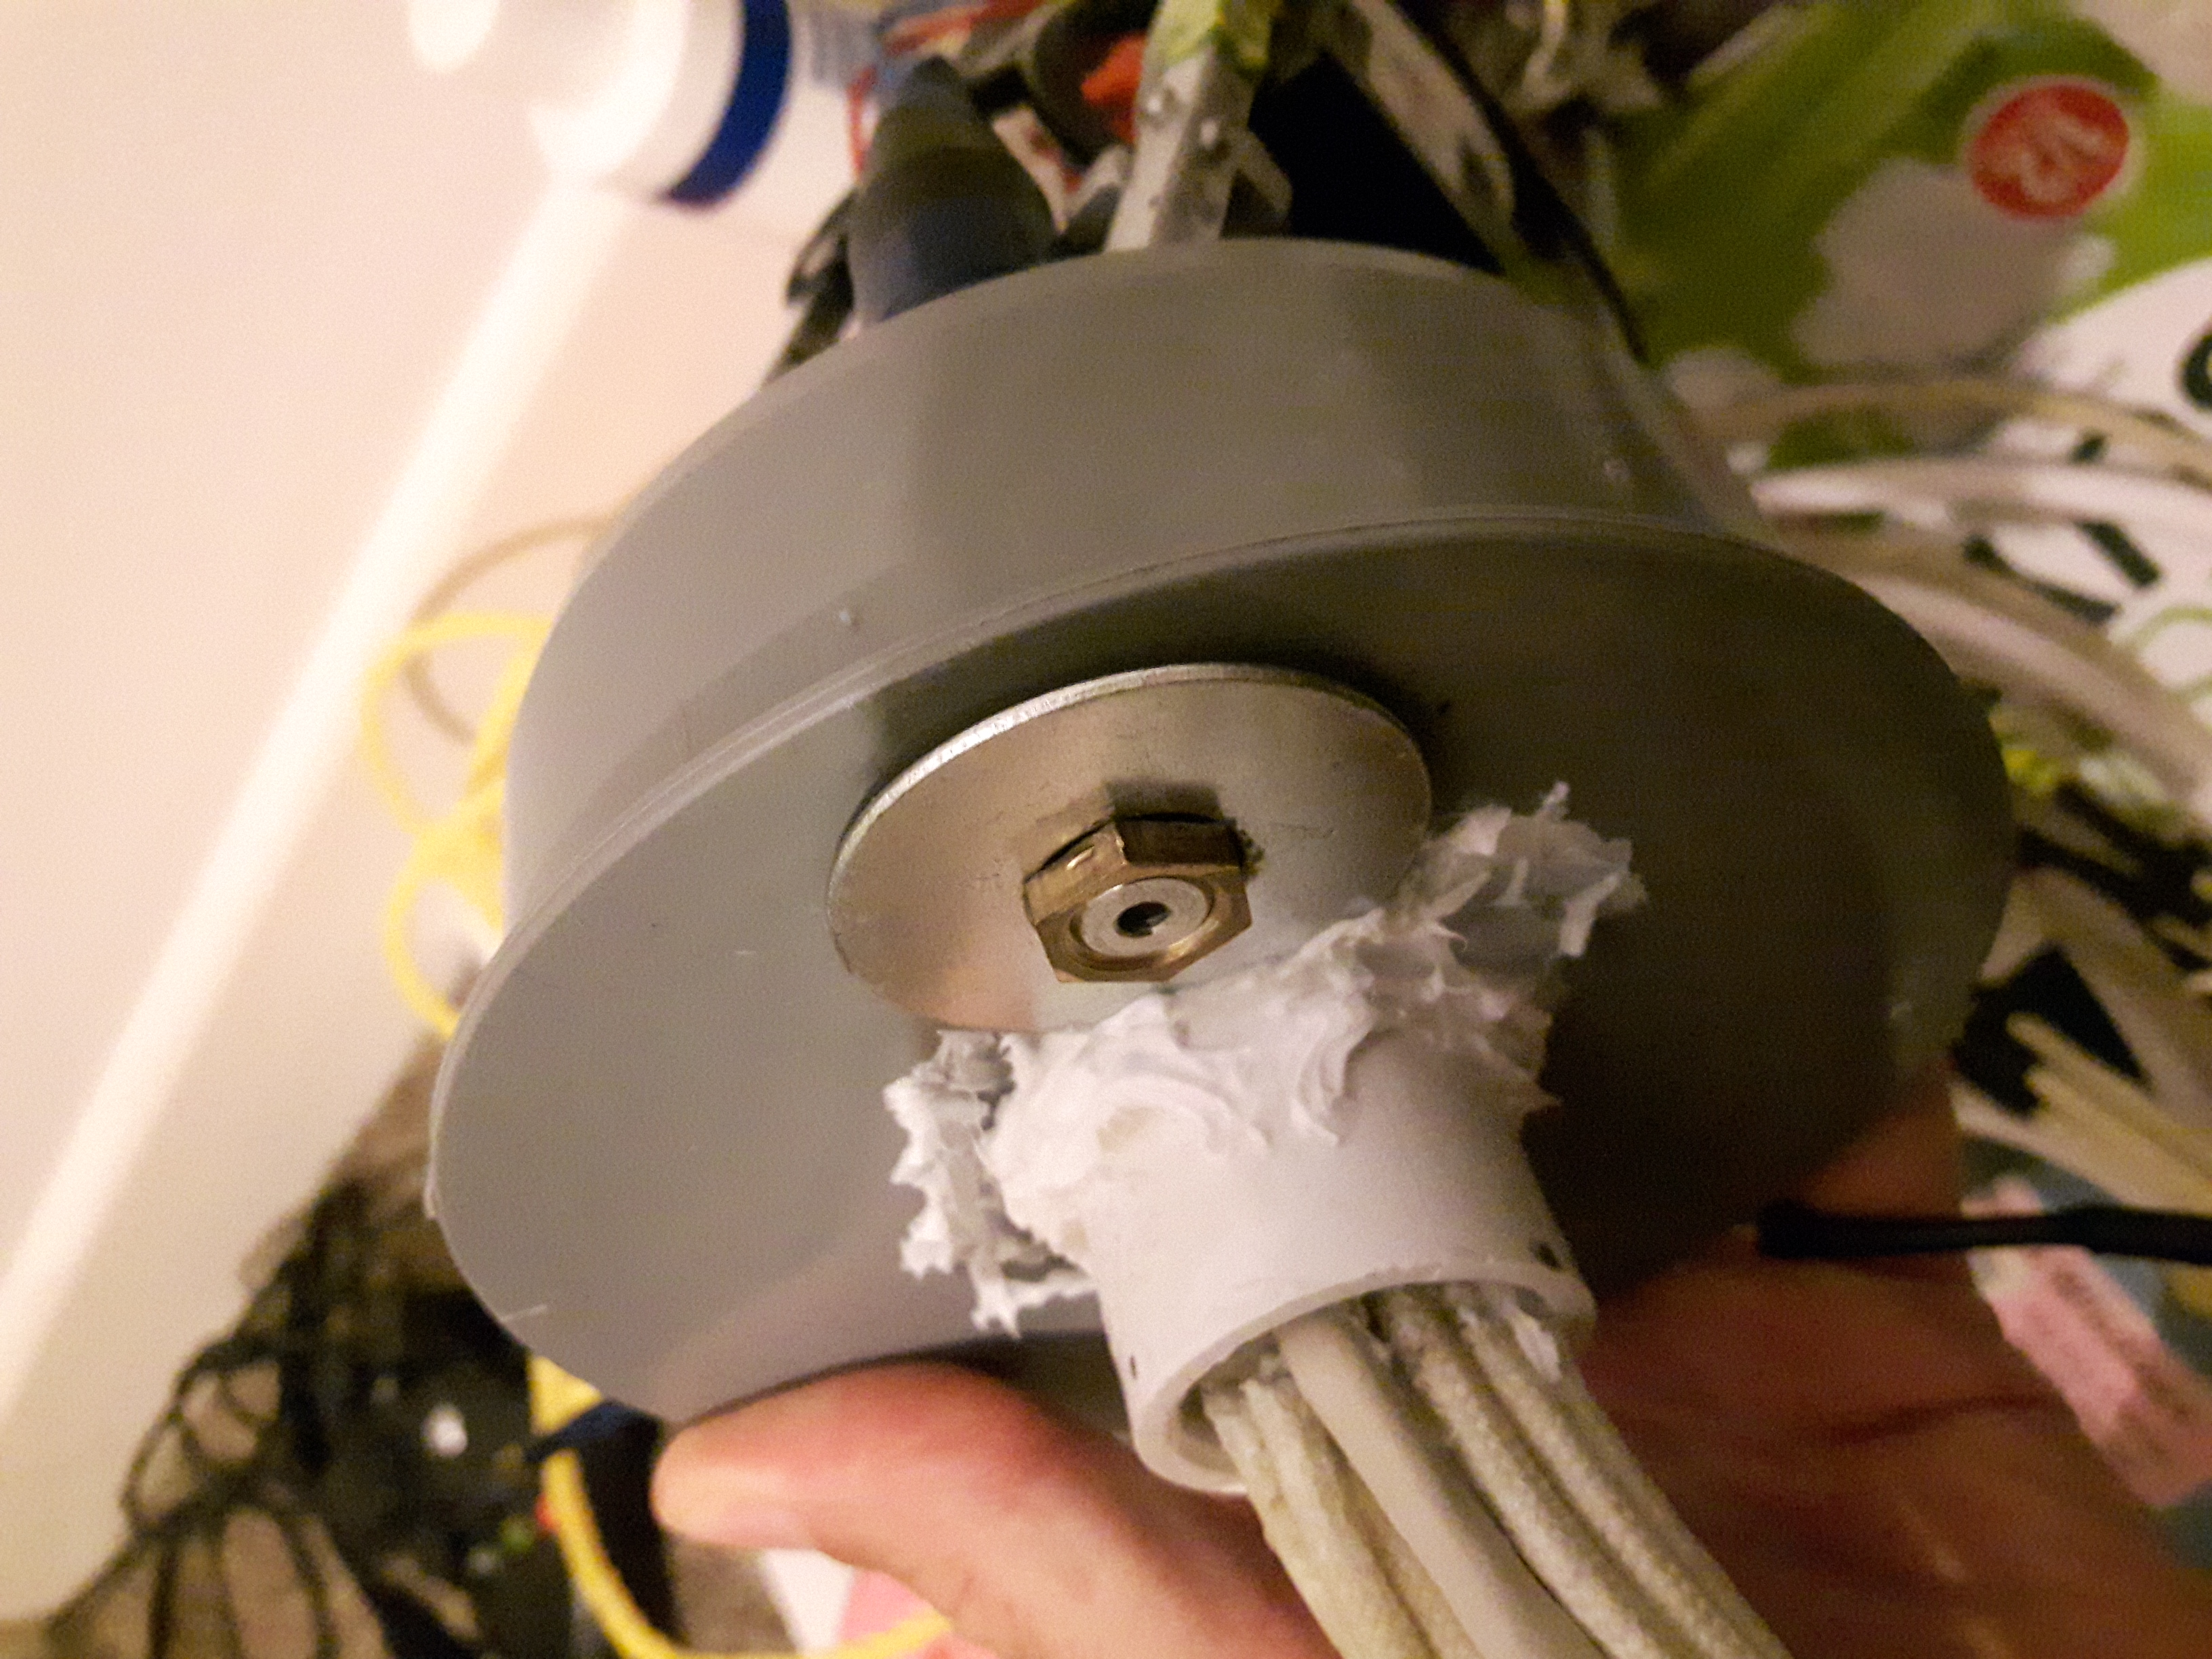
\includegraphics[width=\linewidth,angle=270]{20160827_212715.jpg}
\end{minipage}
\caption{External side of the aft plug with the pressure sensor and umbilical connector mounted.}
\label{fig:externalSideOfTheAftPlug}
\end{figure}

\begin{figure}[htb]
\begin{minipage}[b]{1\linewidth}
  \centering
	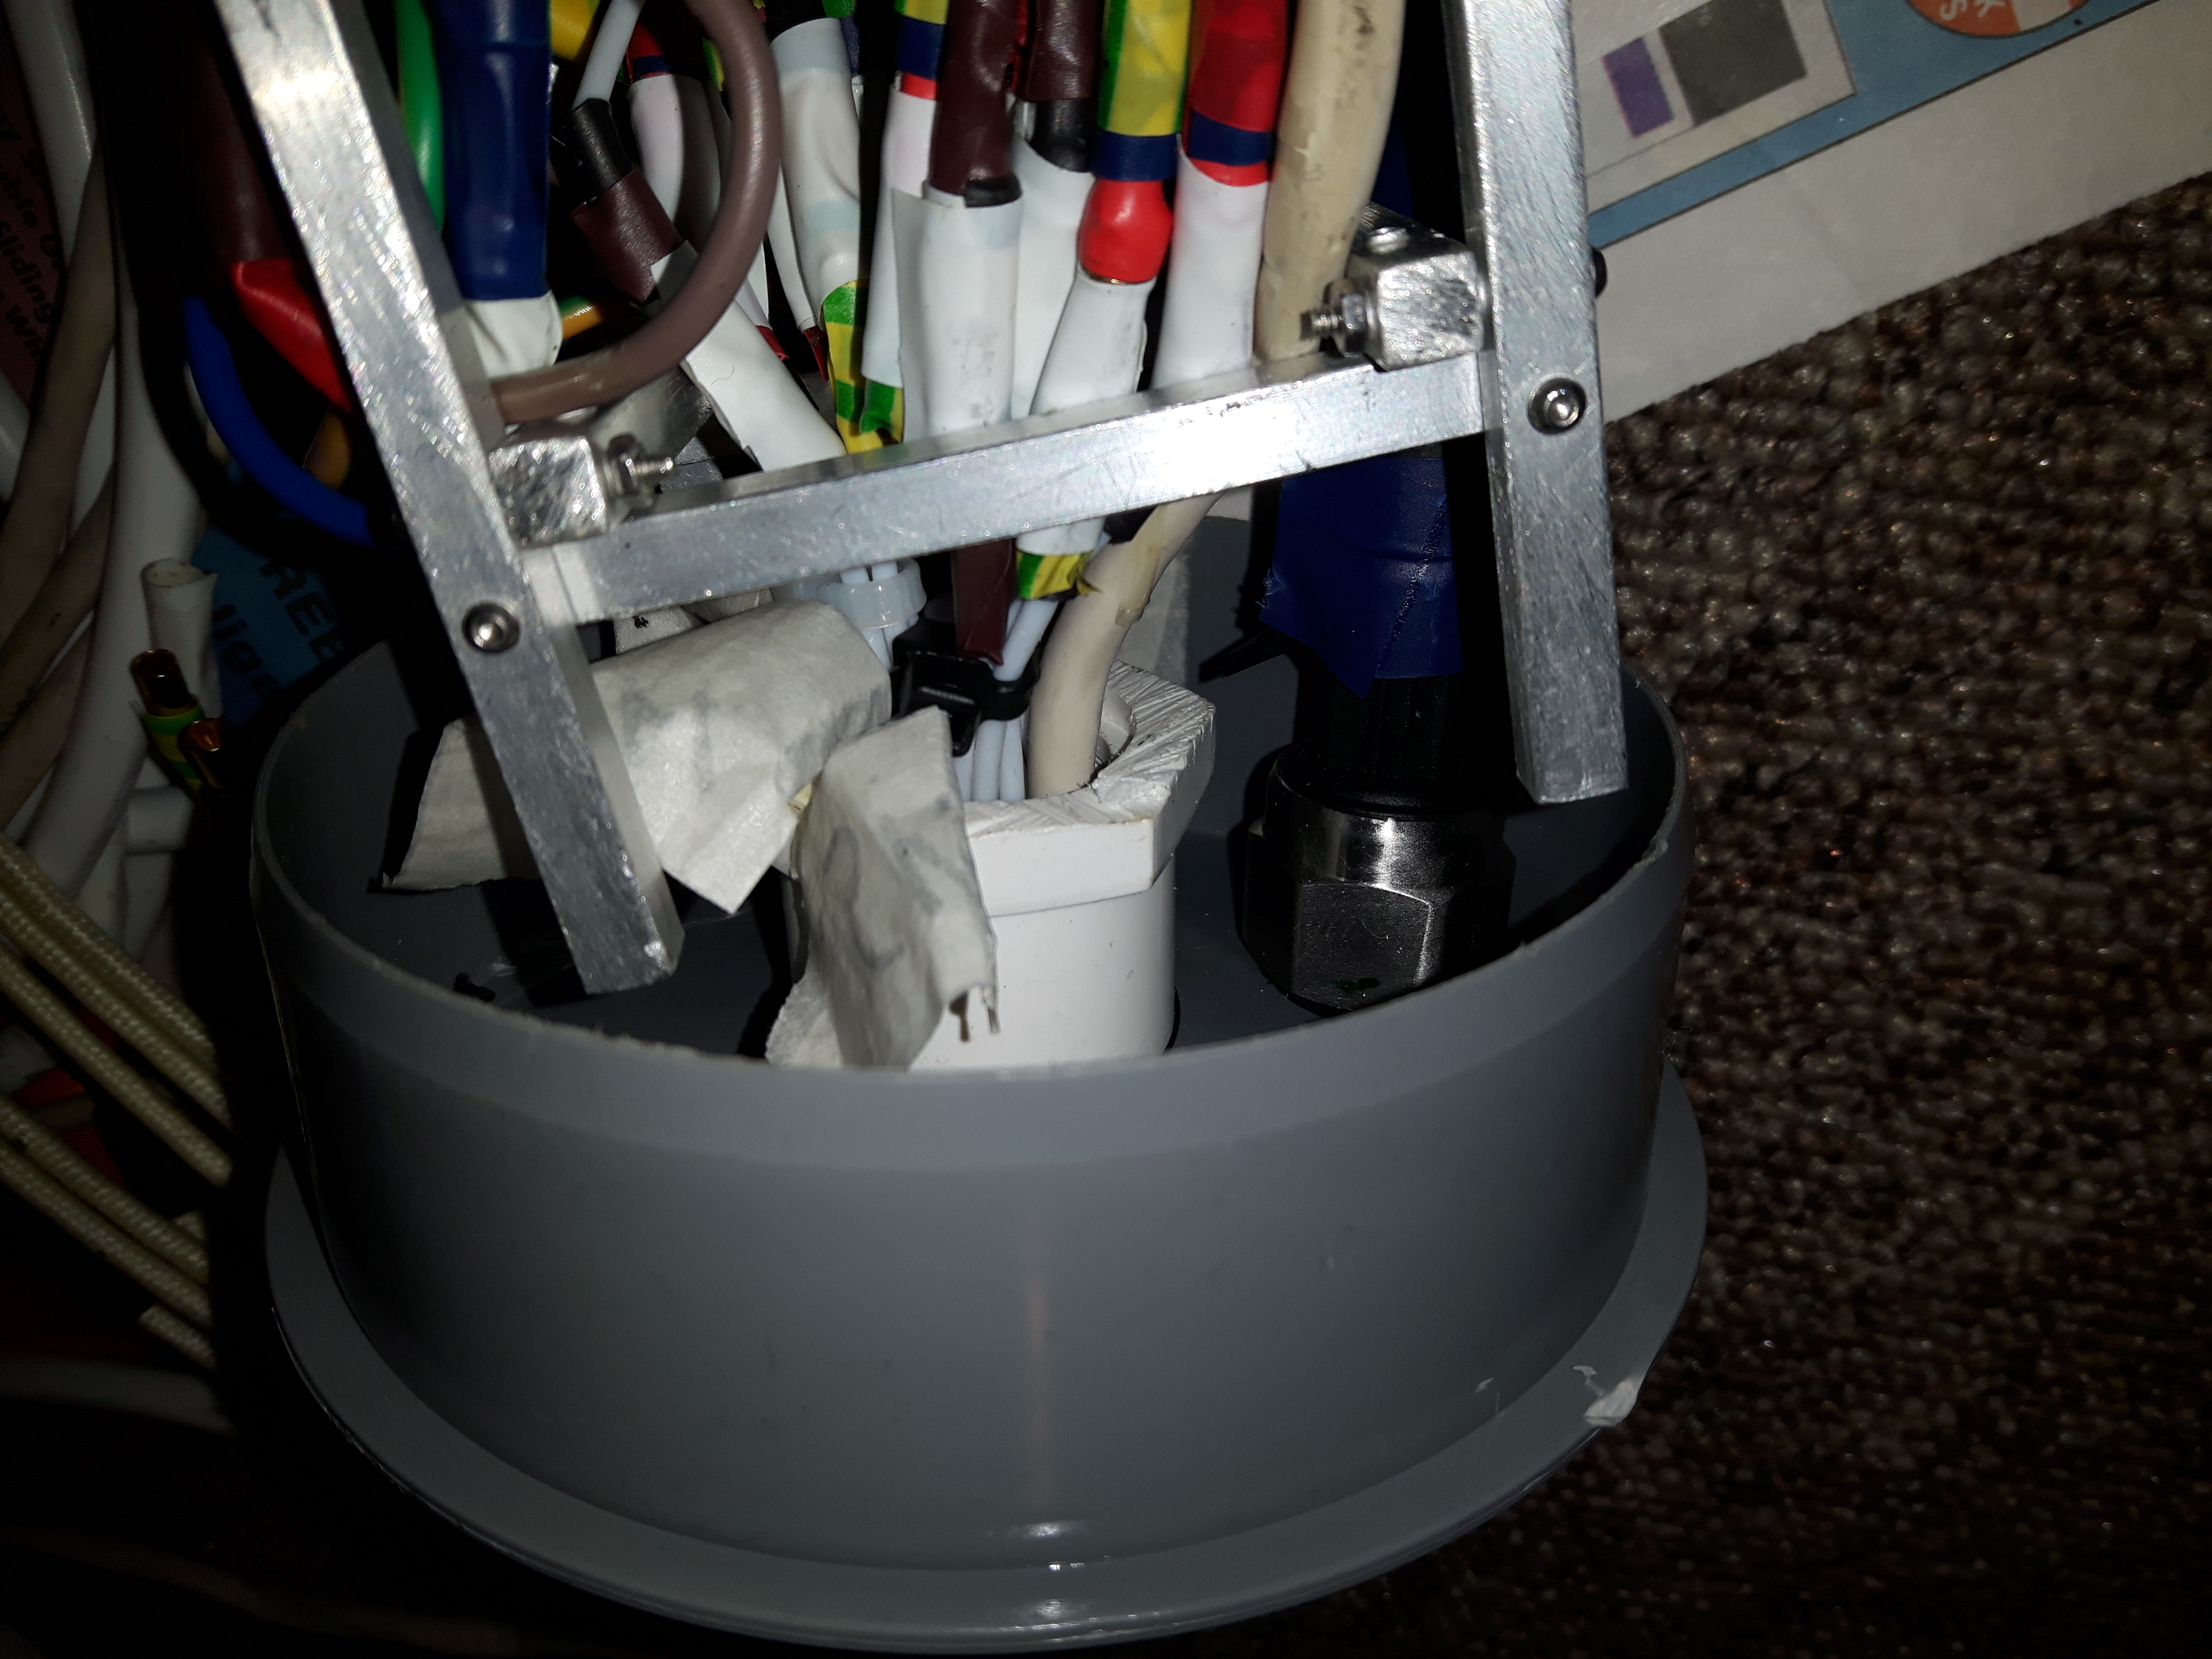
\includegraphics[width=\linewidth,angle=180]{20160827_213602.jpg}
\end{minipage}
\caption{Internal side of the aft plug with the pressure sensor and umbilical connectors mounted. The CAT5 cable is plugged into the USB range extender, and all motor wires are connected to the ESCs and the motor control board.}
\label{fig:internalSideOfTheAftPlug}
\end{figure}

\begin{figure}[htb]
\begin{minipage}[b]{1\linewidth}
  \centering
	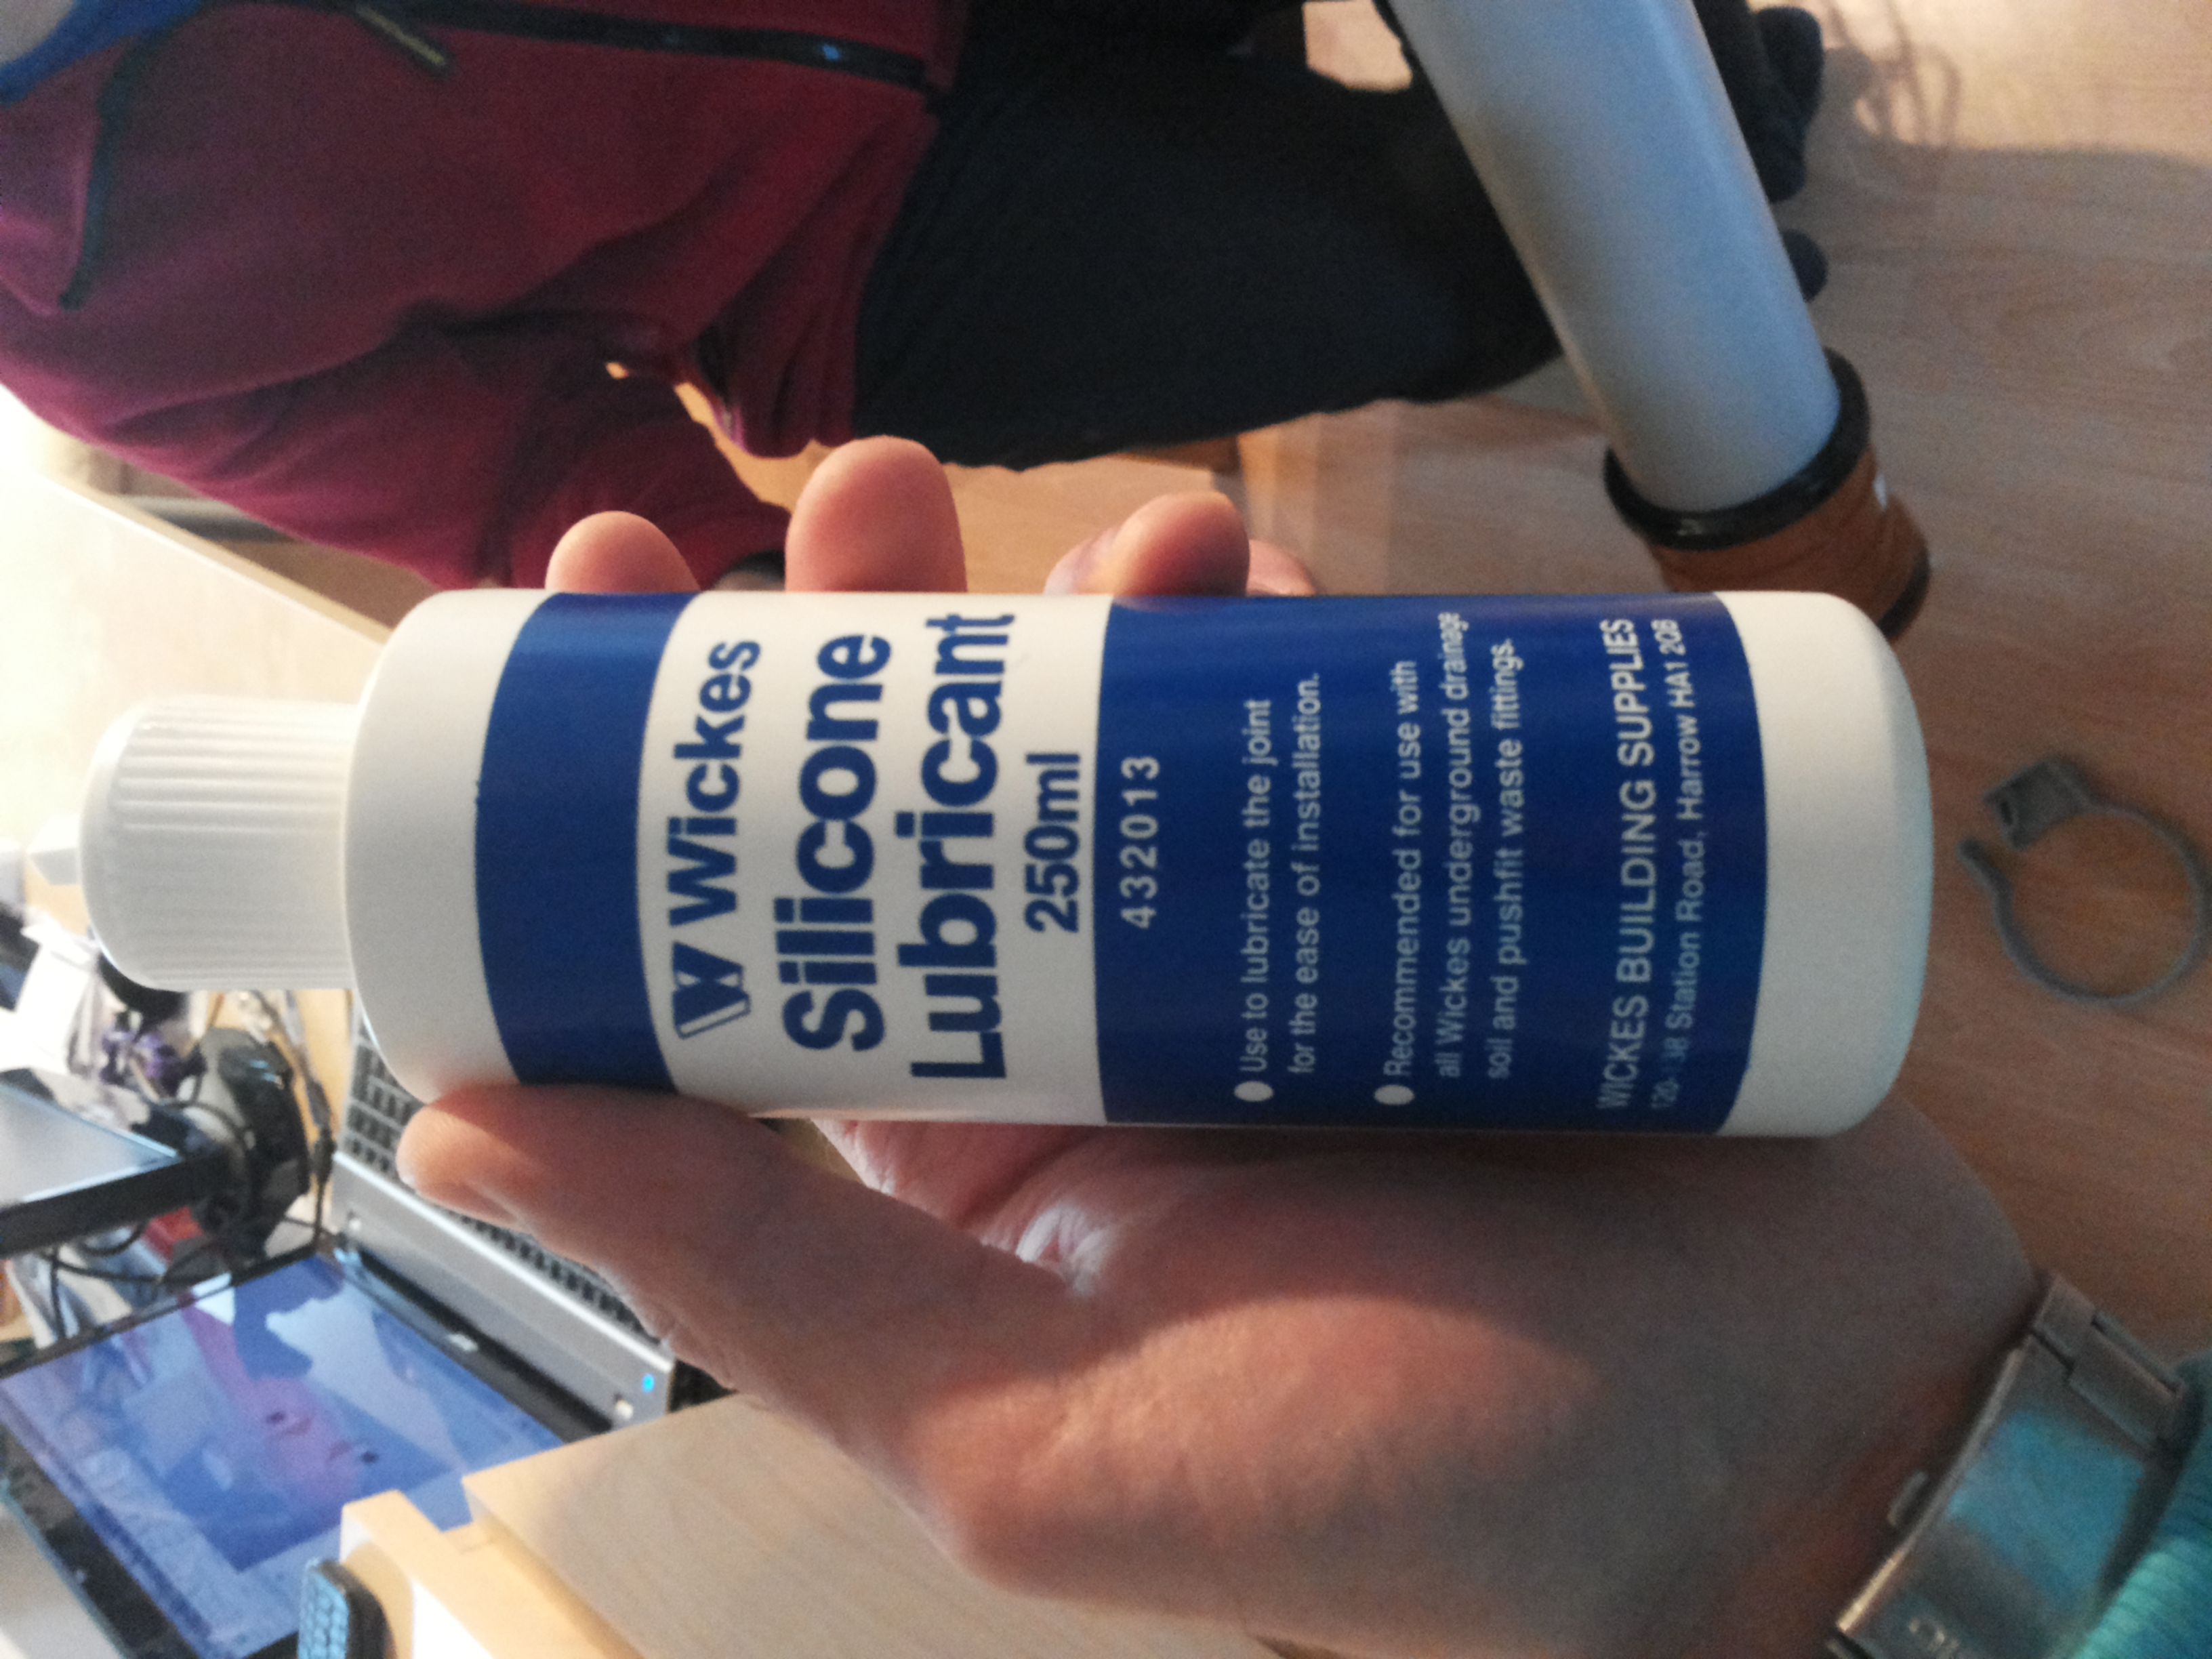
\includegraphics[width=\linewidth,angle=270]{20151122_144346.jpg}
\end{minipage}
\caption{When the aft plug is slid into the main pressure vessel, this silicone lubricant is applied onto it to ease the assembly and improve the seal.}
\label{fig:lubricant}
\end{figure}

%-------------------------------------------------------------------------------
\subsection{Forward plug}\label{ssection:forwardPlug}
The forward plug was manufactured from a~socket plug identical to the one used for manufacture of the aft plug (shown in Fig.~\ref{fig:socketPlug}). The forward plug has to enable the camera to photograph the space in front of the ROV to enable remote operation. To this end, a~hole was cut in the socket plug as shown in Fig.~\ref{fig:cuttingAHole}. A~window was cut out of a~\unit[4]{mm} thick plexiglass, which was glued onto the outer side of the socket plug using a~two-part epoxy glue. The complete forward plug is fixed in the pressure vessel using silicone; this provides both structural strength and makes the connection water-tight. The complete forward plug, mounted into the pressure vessel, can be seen in Fig.~\ref{fig:assembledPressureVessel}.

\begin{figure}[htb]
\begin{minipage}[b]{1\linewidth}
  \centering
	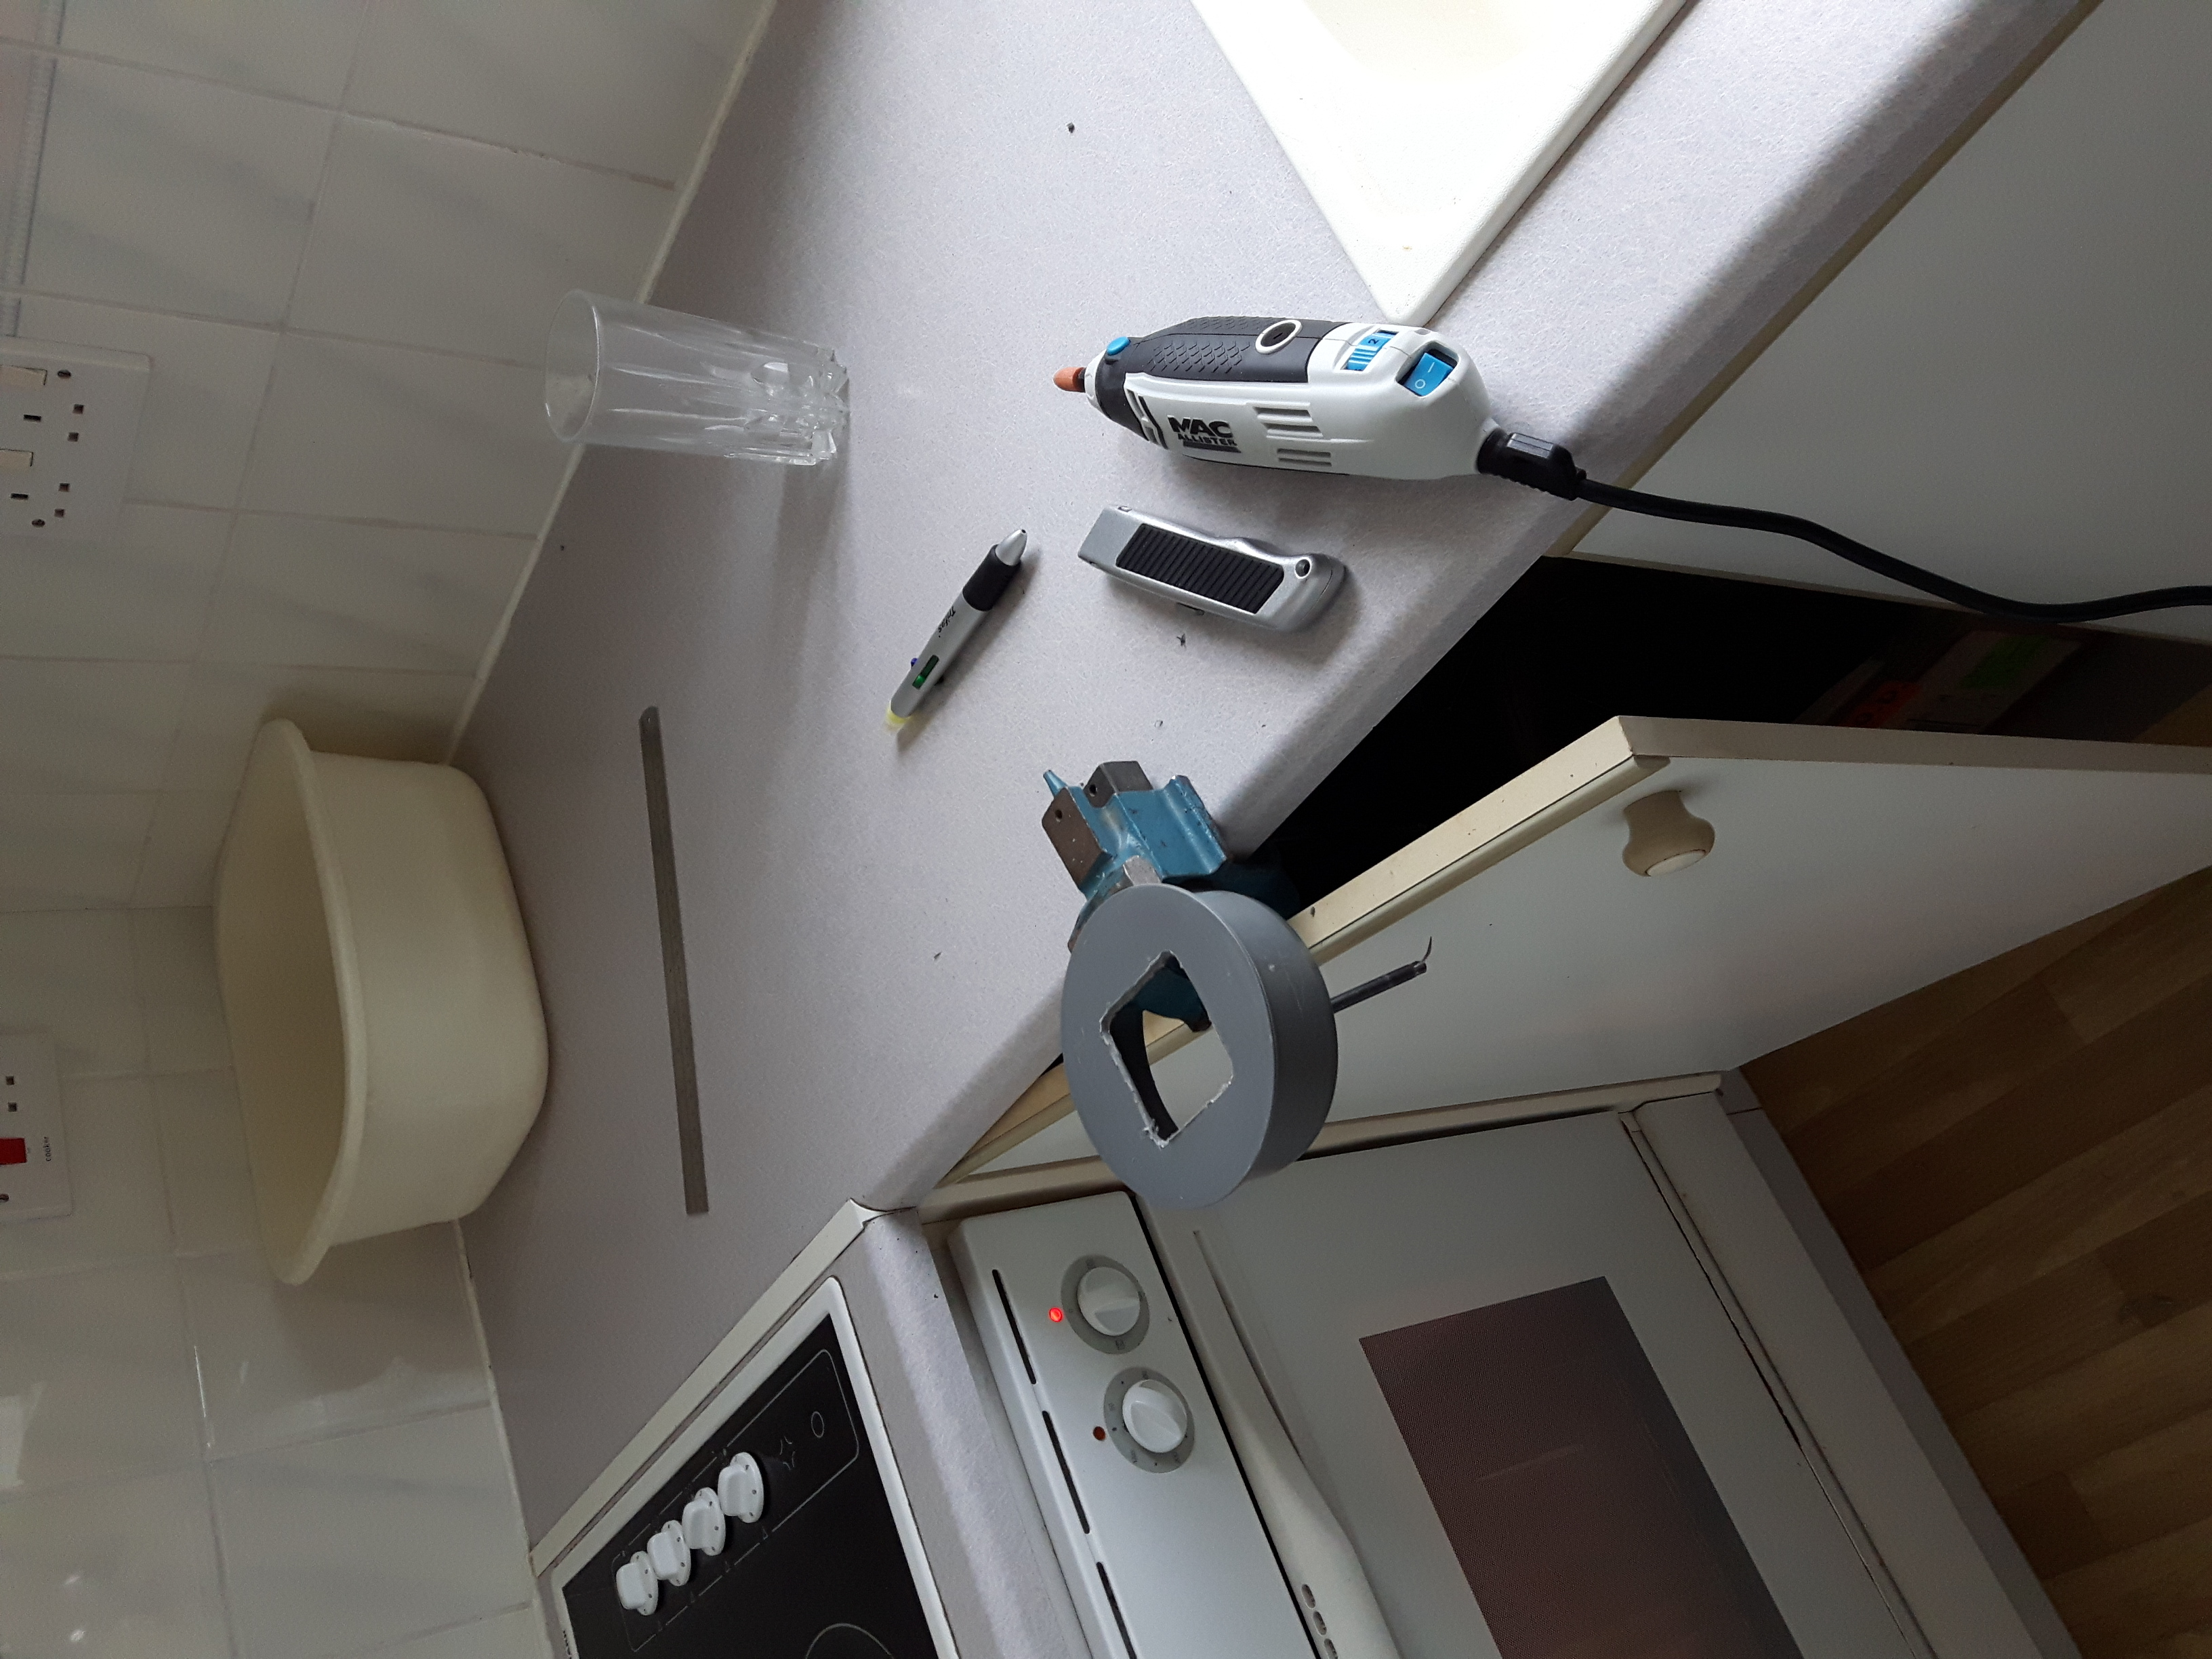
\includegraphics[width=\linewidth,angle=270]{20160418_183948.jpg}
\end{minipage}
\caption{Cutting a~hole in the socket plug to provide a~viewing window for the camera.}
\label{fig:cuttingAHole}
\end{figure}

%-------------------------------------------------------------------------------
\subsection{Main vessel}
The main pressure vessel is made of two PVC pipes, shown in Fig.~\ref{fig:pressureVesselPipes}. The orange double-sided socket is located on the bow of the ROV. The grey socket pipe was cut to the right length (to provide sufficient displacement), slid into the orange double socket, and secured using silicone. This connection is water-tight, and provides structural rigidity and strength. The assembled pressure vessel is shown in Fig.~\ref{fig:assembledPressureVessel}.

Apparently, PVC pipes of the same dimensions can have different masses, depending on their manufacturer. The ones used for this ROV were bought at Wickes, a~UK DIY supermarket.

\begin{figure}[htb]
\begin{minipage}[b]{1\linewidth}
  \centering
	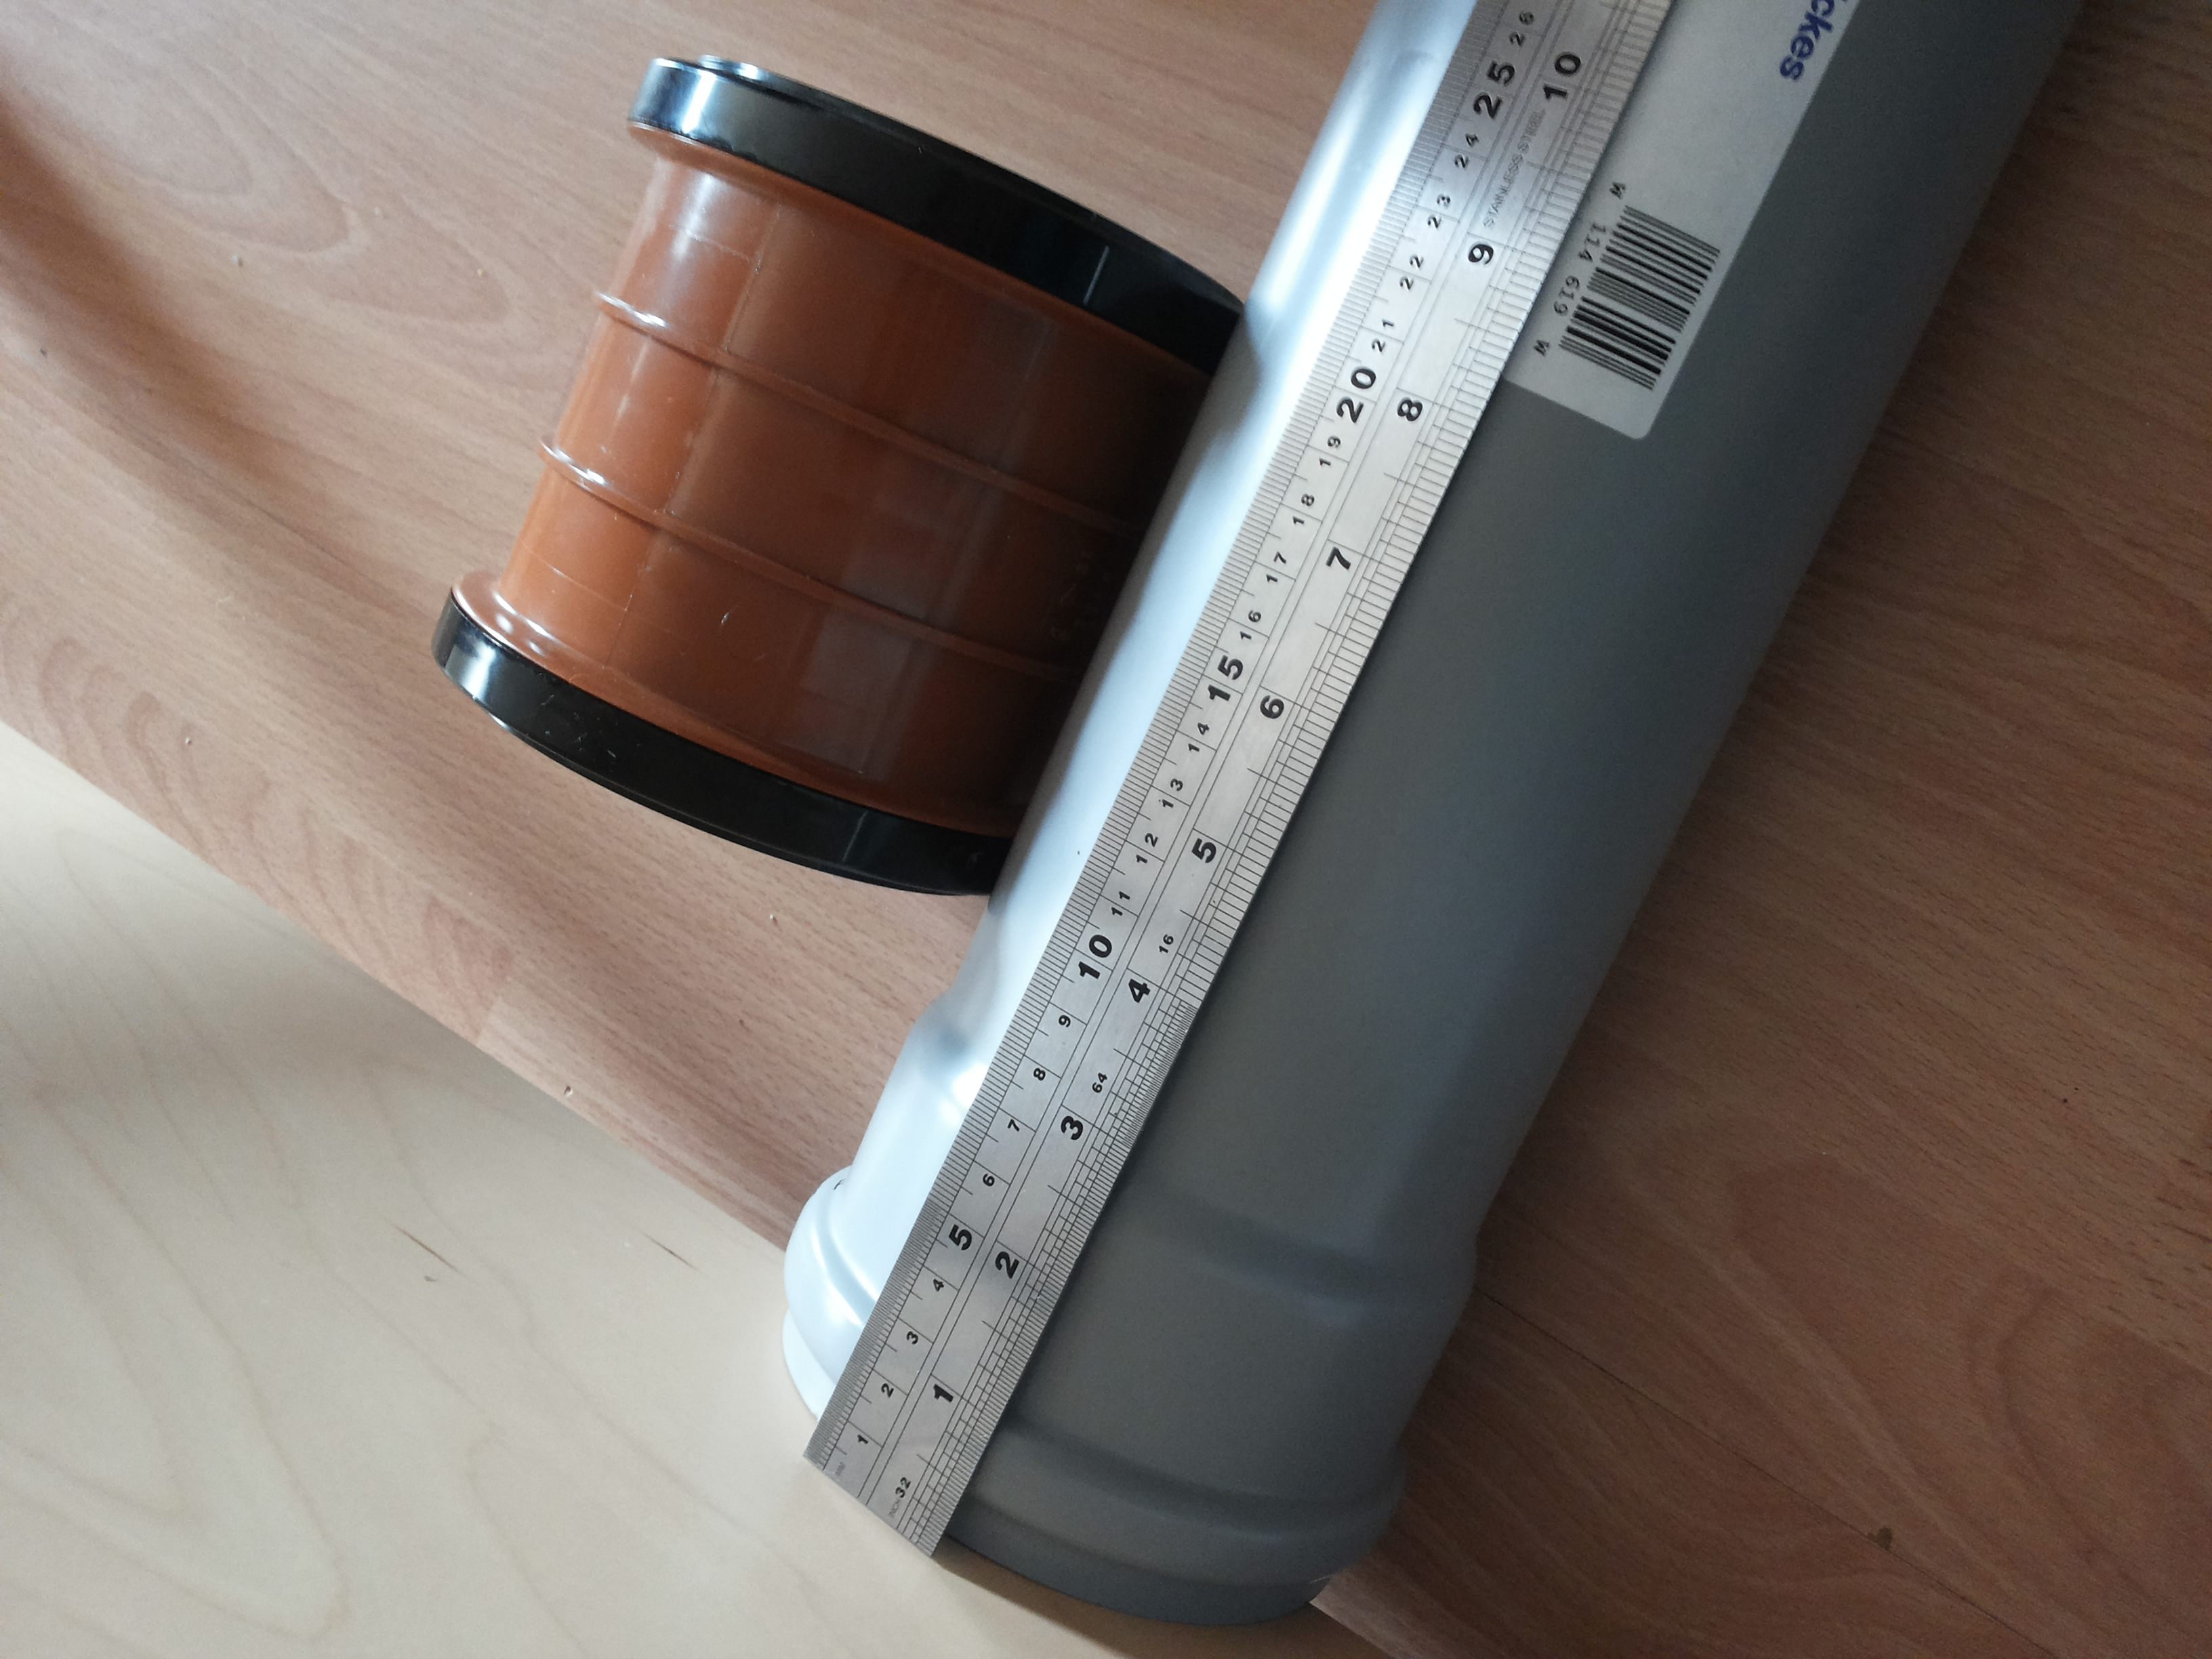
\includegraphics[width=\linewidth]{20151122_142423.jpg}
\end{minipage}
\caption{The pressure vessel consists of two main parts - an orange double-sided socket and a~grey socket pipe.}
\label{fig:pressureVesselPipes}
\end{figure}

\begin{figure}[htb]
\begin{minipage}[b]{1\linewidth}
  \centering
	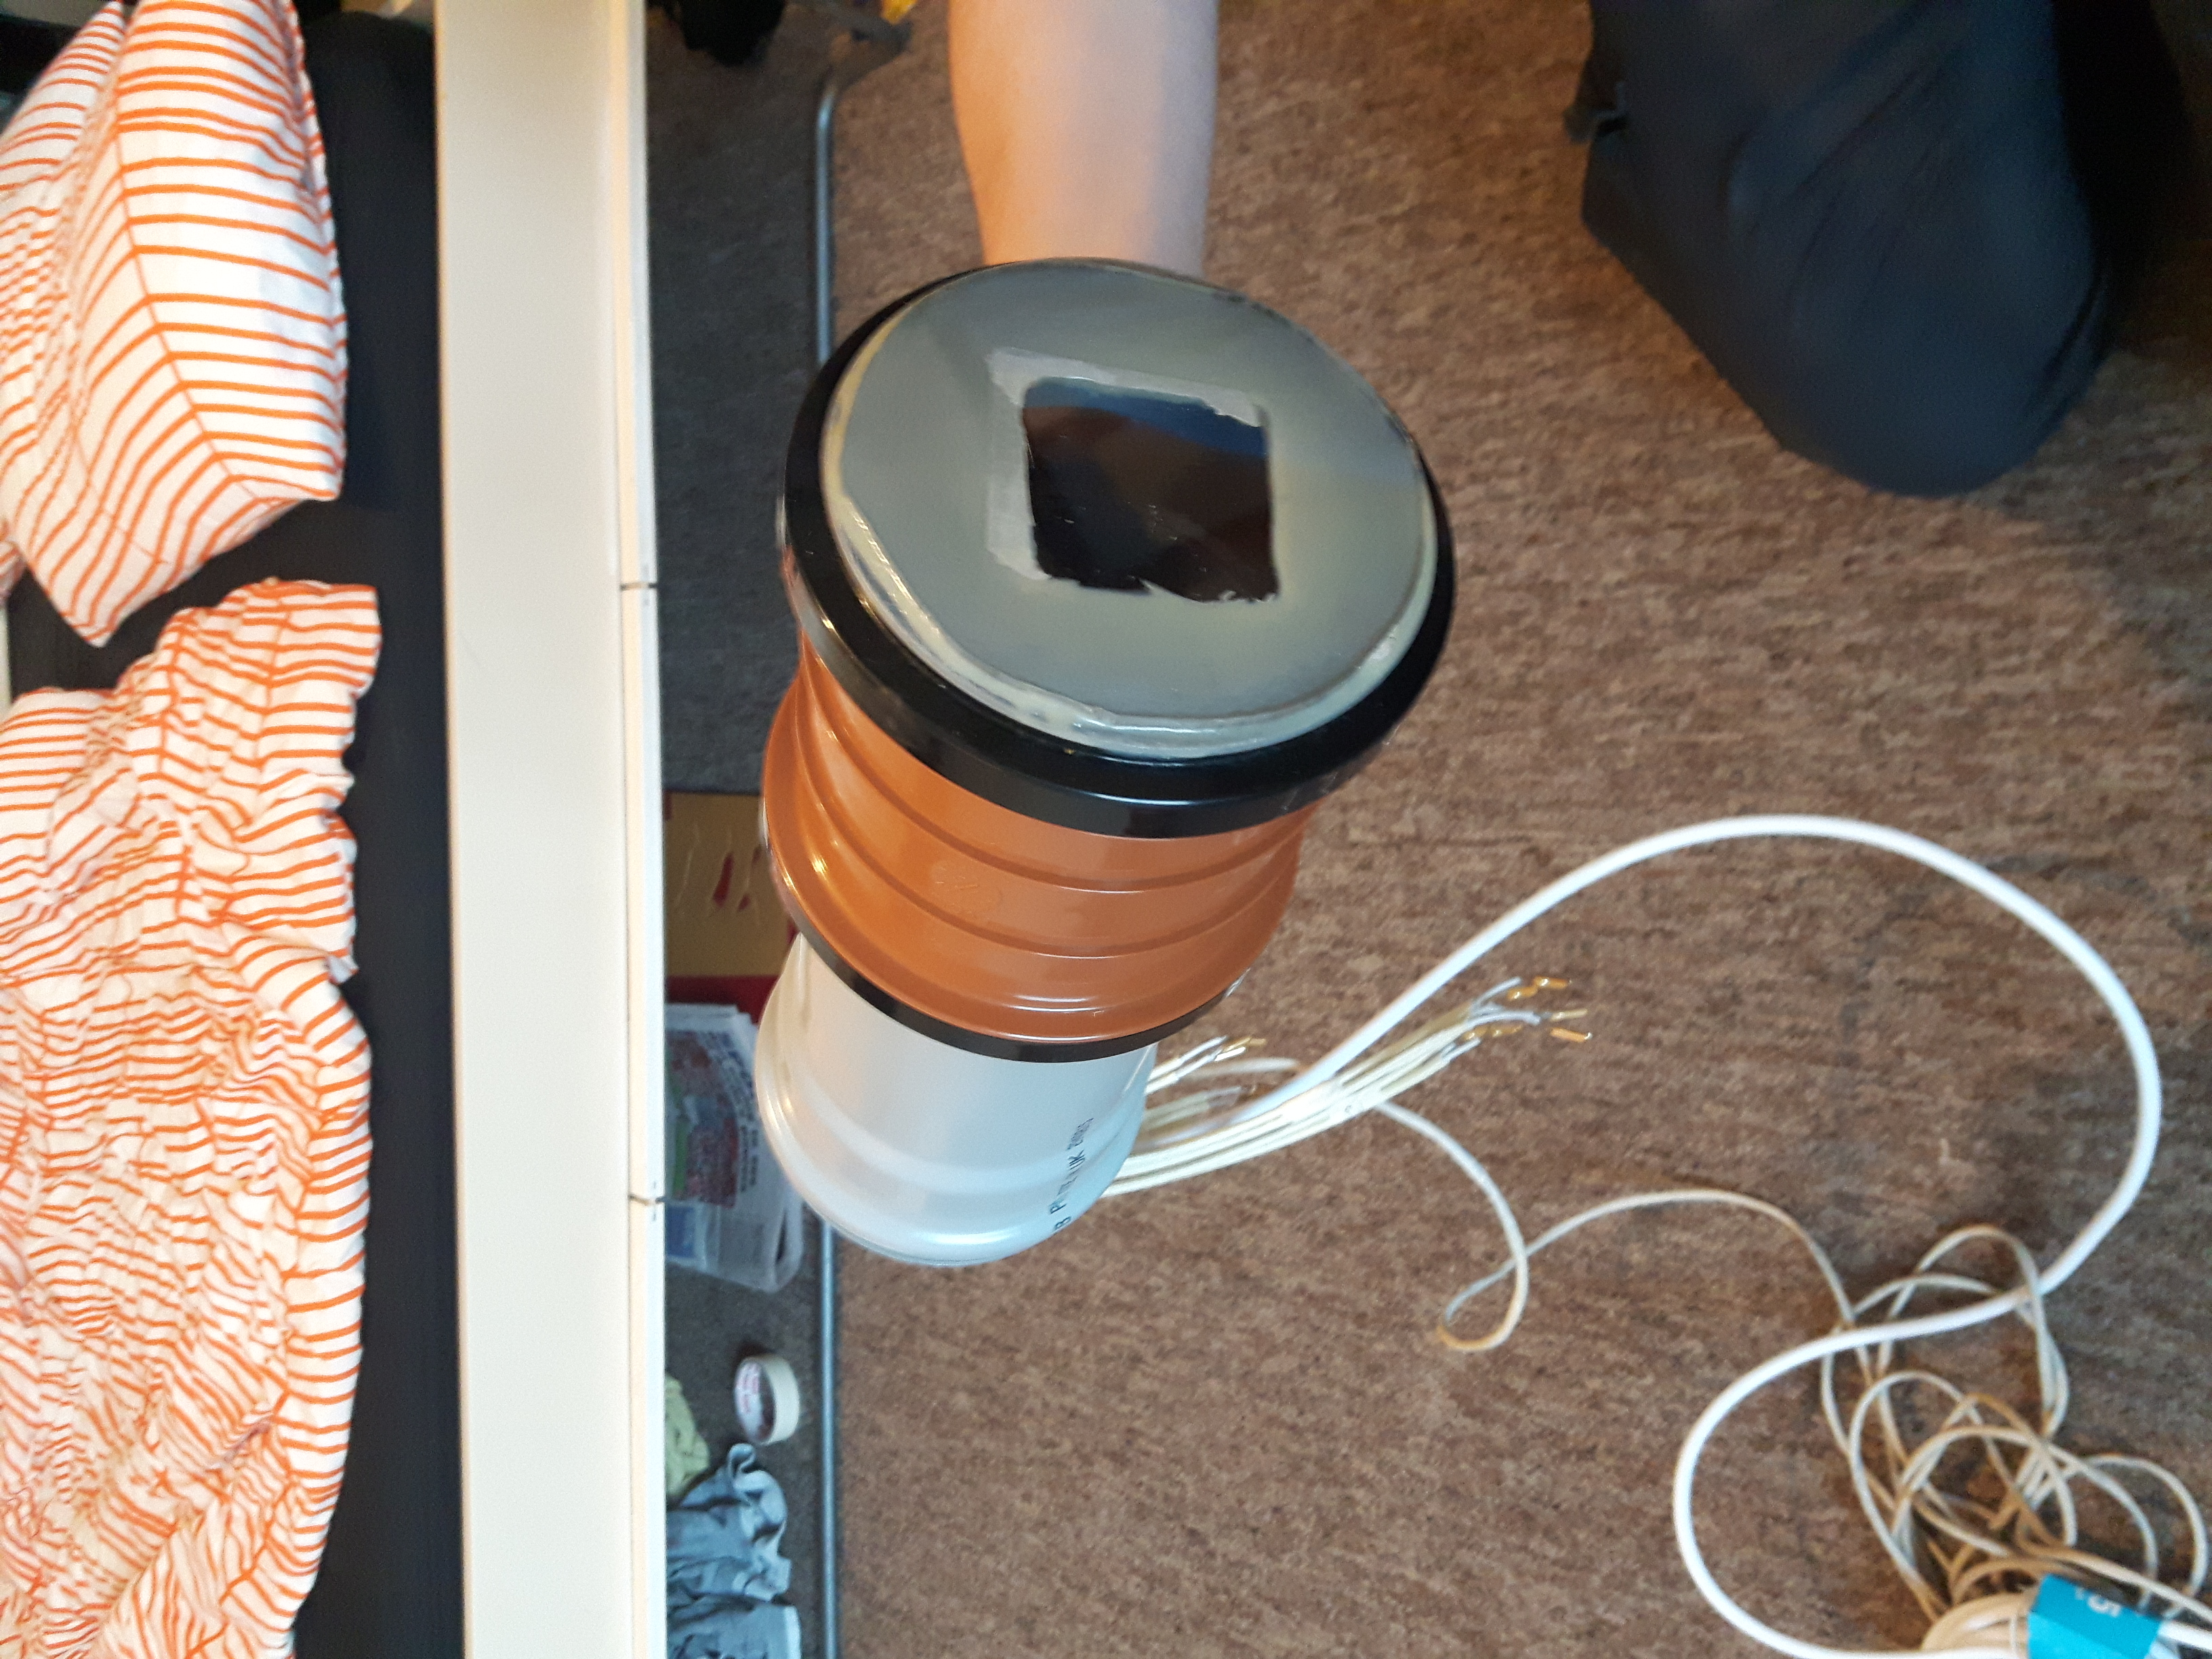
\includegraphics[width=\linewidth,angle=270]{20160507_195201.jpg}
\end{minipage}
\caption{Assembled pressure vessel.}
\label{fig:assembledPressureVessel}
\end{figure}

\clearpage % Avoid "too many unprocessed floats" error.

%===============================================================================
\section{External structure}\label{section:externalStructure}
For the naming convention and location of the components of the external structure, please refer to Fig.~\ref{fig:rovGAsExternal}.

%-------------------------------------------------------------------------------
\subsection{Transversals and longitudinals}
Side longitudinals, trasnverse clip stiffeners, and landing sleds were made of \unit[2]{mm} thick, \unit[20]{mm} wide rolled steel. In order to reduce their mass, M10 holes were drilled along their lengths. The structure is bolted together using M3 bolts. All the metal parts are painted to reduce corrosion.

%-------------------------------------------------------------------------------
\subsection{Pressure vessel mounting}
In order to mate the external metal structure with the pressure vessel made of PVC pipes, PVC socket brackets are used. The landing sleds and transversal clip stiffeners are bolted onto the default mounting holes in the brackets, which can be seen on the bottom of Fig.~\ref{fig:motorMountingDetails:label:a}. In order to mount the side longitudinals and motors, additional M3 holes were drilled in the socket brackets, as shown in Fig.~\ref{fig:brackets} and Fig.~\ref{fig:motorMountingDetails:label:a}.

The steel structure was bolted together and onto the socket brackets, but one side of every bracket was left free (one bolt going through the landing sled and transverse clip stiffener was not inserted). Then, the pressure vessel was inserted into the brackets, and the loose end of every bracket was fixed in place around the pressure vessel by bolting it onto the sled and the transverse clip stiffener.

To prevent the steel structure from slipping along the pressure vessel, the bow bracket was placed in the groove in the double socket pipe, as shown in Fig.~\ref{fig:brackets}. To stop the brackets from rotating around the pressure vessel, both of them were glued to it using a~two-part epoxy glue.

\begin{figure}[htb]
\begin{minipage}[b]{1\linewidth}
  \centering
	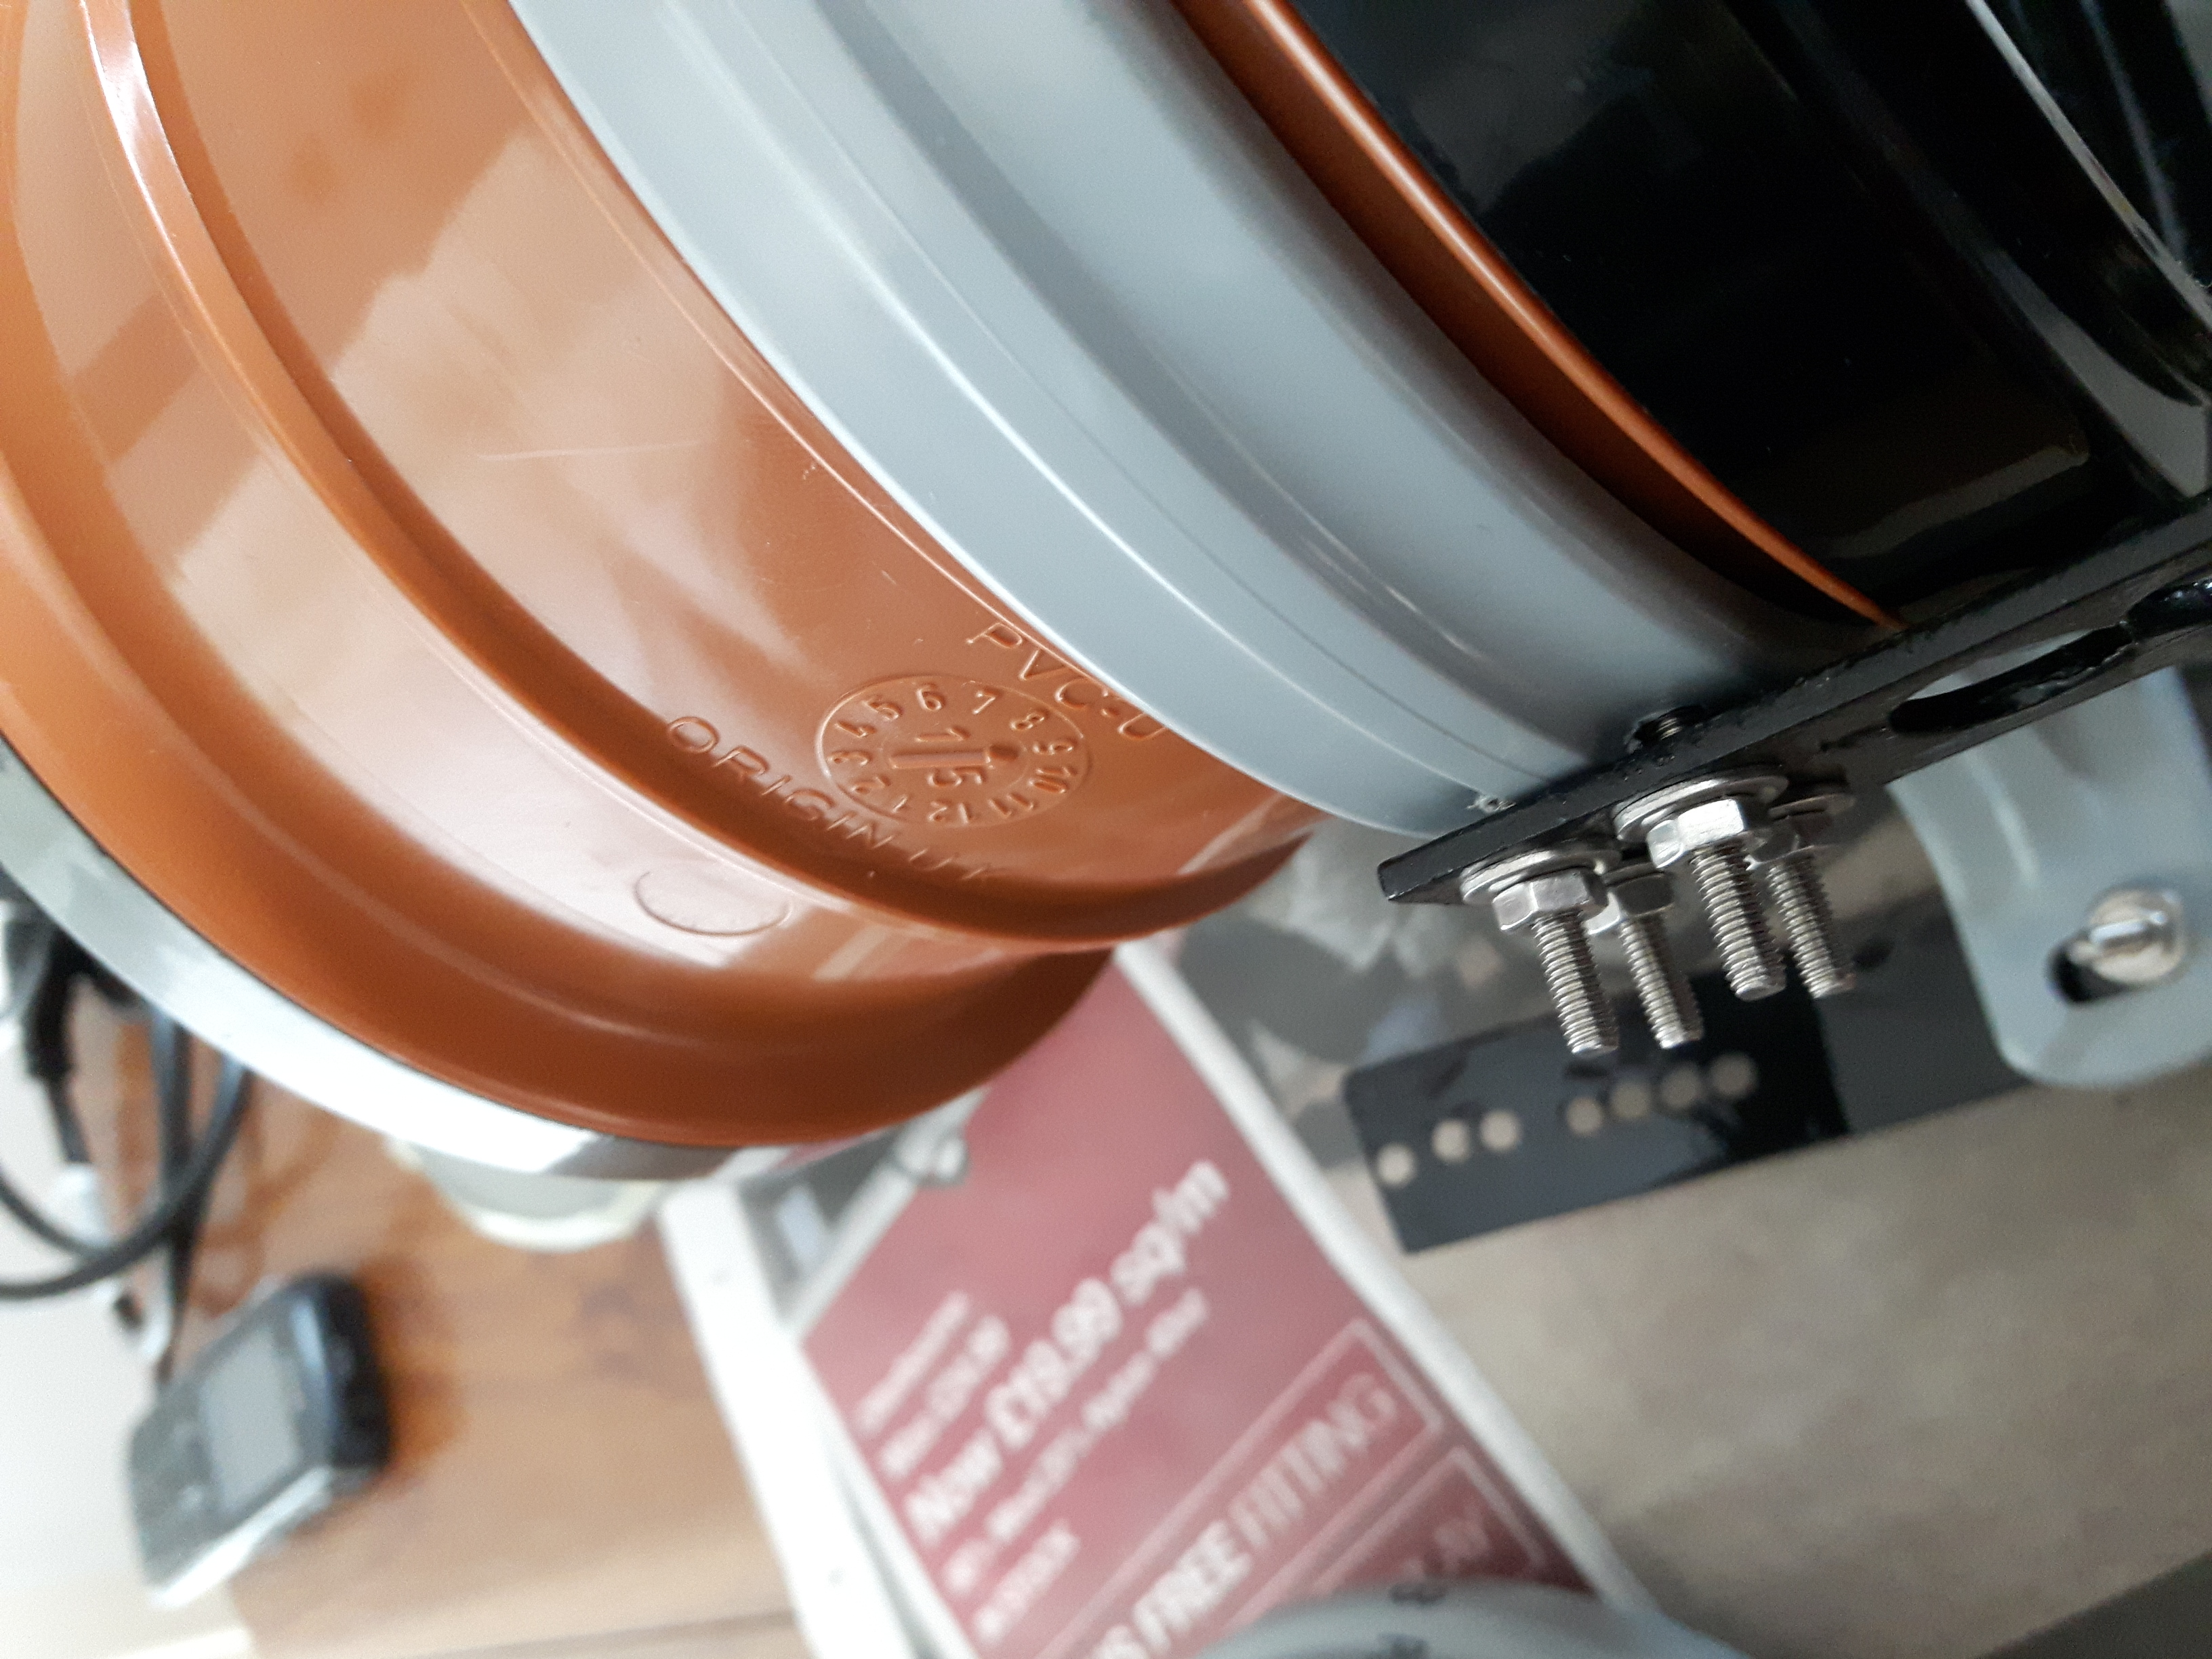
\includegraphics[width=\linewidth]{20160625_143939.jpg}
\end{minipage}
\caption{Using socket brackets to mount the steel structure onto the pressure vessel. One of the brackets is placed in the grooves in the double-socket pipe to stop them from slipping along the ROV.}
\label{fig:brackets}
\end{figure}

%-------------------------------------------------------------------------------
\subsection{Motor mounting}
Motors are bolted onto custom brackets made of bent steel (\unit[2 by 20]{mm} section) using M2.5 bolts. The motor manufacturer does not provide a~detailed drawing that specifies the location of the mounting holes. Therefore, the location of the holes was marked on the brackets by using the motors themselves as a~guide. To ensure that the motors rotate freely, they are separated from their brackets using two washers, as shown in Fig.~\ref{fig:motorMountingDetails:label:b}.

The vertical motor brackets are located in the approximate longitudinal centre of buoyancy (centre of the pressure vessel) to reduce the pitching moment that the vertical motors impart on the vehicle. Similarly, the horizontal motor brackets are mounted at the vertical centre of buoyancy. To reduce the number of the holes in the socket brackets, both sets of motor brackets are bolted onto the side longitudinals, which are then bolted onto the socket brackets, as shown in Fig.~\ref{fig:motorMountingDetails}.

\begin{figure}[htb]
\begin{center}
\begin{tabular}{c c}
	\subfloat[Back]
		{\includegraphics*[width=0.6\textwidth,angle=270]{20160625_143911.jpg}
		\label{fig:motorMountingDetails:label:a} } &
	\subfloat[Top]
		{\includegraphics*[width=0.6\textwidth,angle=270]{20160625_143928.jpg}
		\label{fig:motorMountingDetails:label:b} } \\
\end{tabular}
\end{center}
\caption{Details of mounting the motors onto the external steel structure. Views from the top and back of the vehicle.}
\label{fig:motorMountingDetails}
\end{figure}

%-------------------------------------------------------------------------------
\subsection{Ballast}
The ballast consists of two sets of elements: \unit[4 by 30]{mm} rolled steel flat-bar section cut to the length of the transverse clip stiffeners, and a~\unit[186]{mm} long, \unit[2 by 20]{mm} steel bar. The latter was a~left-over from the steel bought to manufacture the external frame.

Five of the \unit[4 by 30]{mm} sections are mounted close to the centre of gravity in order to compensate for the excess net buoyancy available from the hull. They are placed slightly forward to balance out the moment generated by the heavy wires and cables placed at the aft end. The smaller ballast bar is placed at the forward end of the sled and its exact position was adjusted to achieve an even trim. This was possible thanks to there being a~series of holes on either side of the sled, which allow fine-tuning of the ballast position. The arrangement of the ballast is indicated in Fig.~\ref{fig:rovGAsExternal}.

\clearpage % Avoid "too many unprocessed floats" error.

%===============================================================================
\section{Umbilical}\label{section:umbilical}

%-------------------------------------------------------------------------------
\subsection{Connector on the ROV}\label{ssection:connectorOnTheROV}
The connector enables the CAT5 cable and the shore power cable, which form the tether described in more detail in section~\ref{ssection:tether}, as well as the wires carrying signals from the ESCs to the motors described in section~\ref{ssection:propulsionSubsystem}, to penetrate inside the pressure vessel without compromising water tightness.

The connector is based on a~threaded PVC connector, the male part of which is shown in Fig.~\ref{fig:pvcConnector}. All the mentioned cables and wires were threaded through the male connector, which was then filled with a~two-part epoxy resin. All the wires were stripped out of their outermost covers as shown in Fig.~\ref{fig:strippingWires} to allow the resin to penetrate as deep into the wires as possible, to reduce the possibility of water dripping into the pressure vessel between the resin and the wires' cores. For the same reasons, the wires were separated from each other when applying the epoxy, as shown in Fig.~\ref{fig:separatingTheWires}. This ensured that some resin was present between all the wires.

Once complete, the male connector with wires laminated-in was screwed into the hole punched in the aft plug from its outer side, with PTFE tape used to seal the thread. Two rubber washers were placed on the connector, on both the inner and outer sides of the aft plug. A~complementary, female part of the PVC connector was then screwed onto the male counterpart to remove the voids between the washers and the PVC parts. Lastly, silicone was applied to the outer side of the aft plug to further seal the connector. The complete aft plug, with the connector screwed in and silicone applied, is shown in Fig.~\ref{fig:externalSideOfTheAftPlug}.

Banana connectors were soldered onto the motor wires. The motor wires were then connected to the motors, and the ESCs and the motor control board (described in section~\ref{ssection:propulsionSubsystem}) such that forward and upward thrust would be produced without the relays on the motor control board being activated. The wires were colour-coded to ease re-assembly in this configuration. Finally, after the final assembly, the wires were fixed using white electrical tape, which also isolates the banana connectors from each other. The colour coding of the motor wires and the white electrical tape can be seen in Fig.~\ref{fig:internalSideOfTheAftPlug}.

\begin{figure}[htb]
\begin{minipage}[b]{1\linewidth}
  \centering
	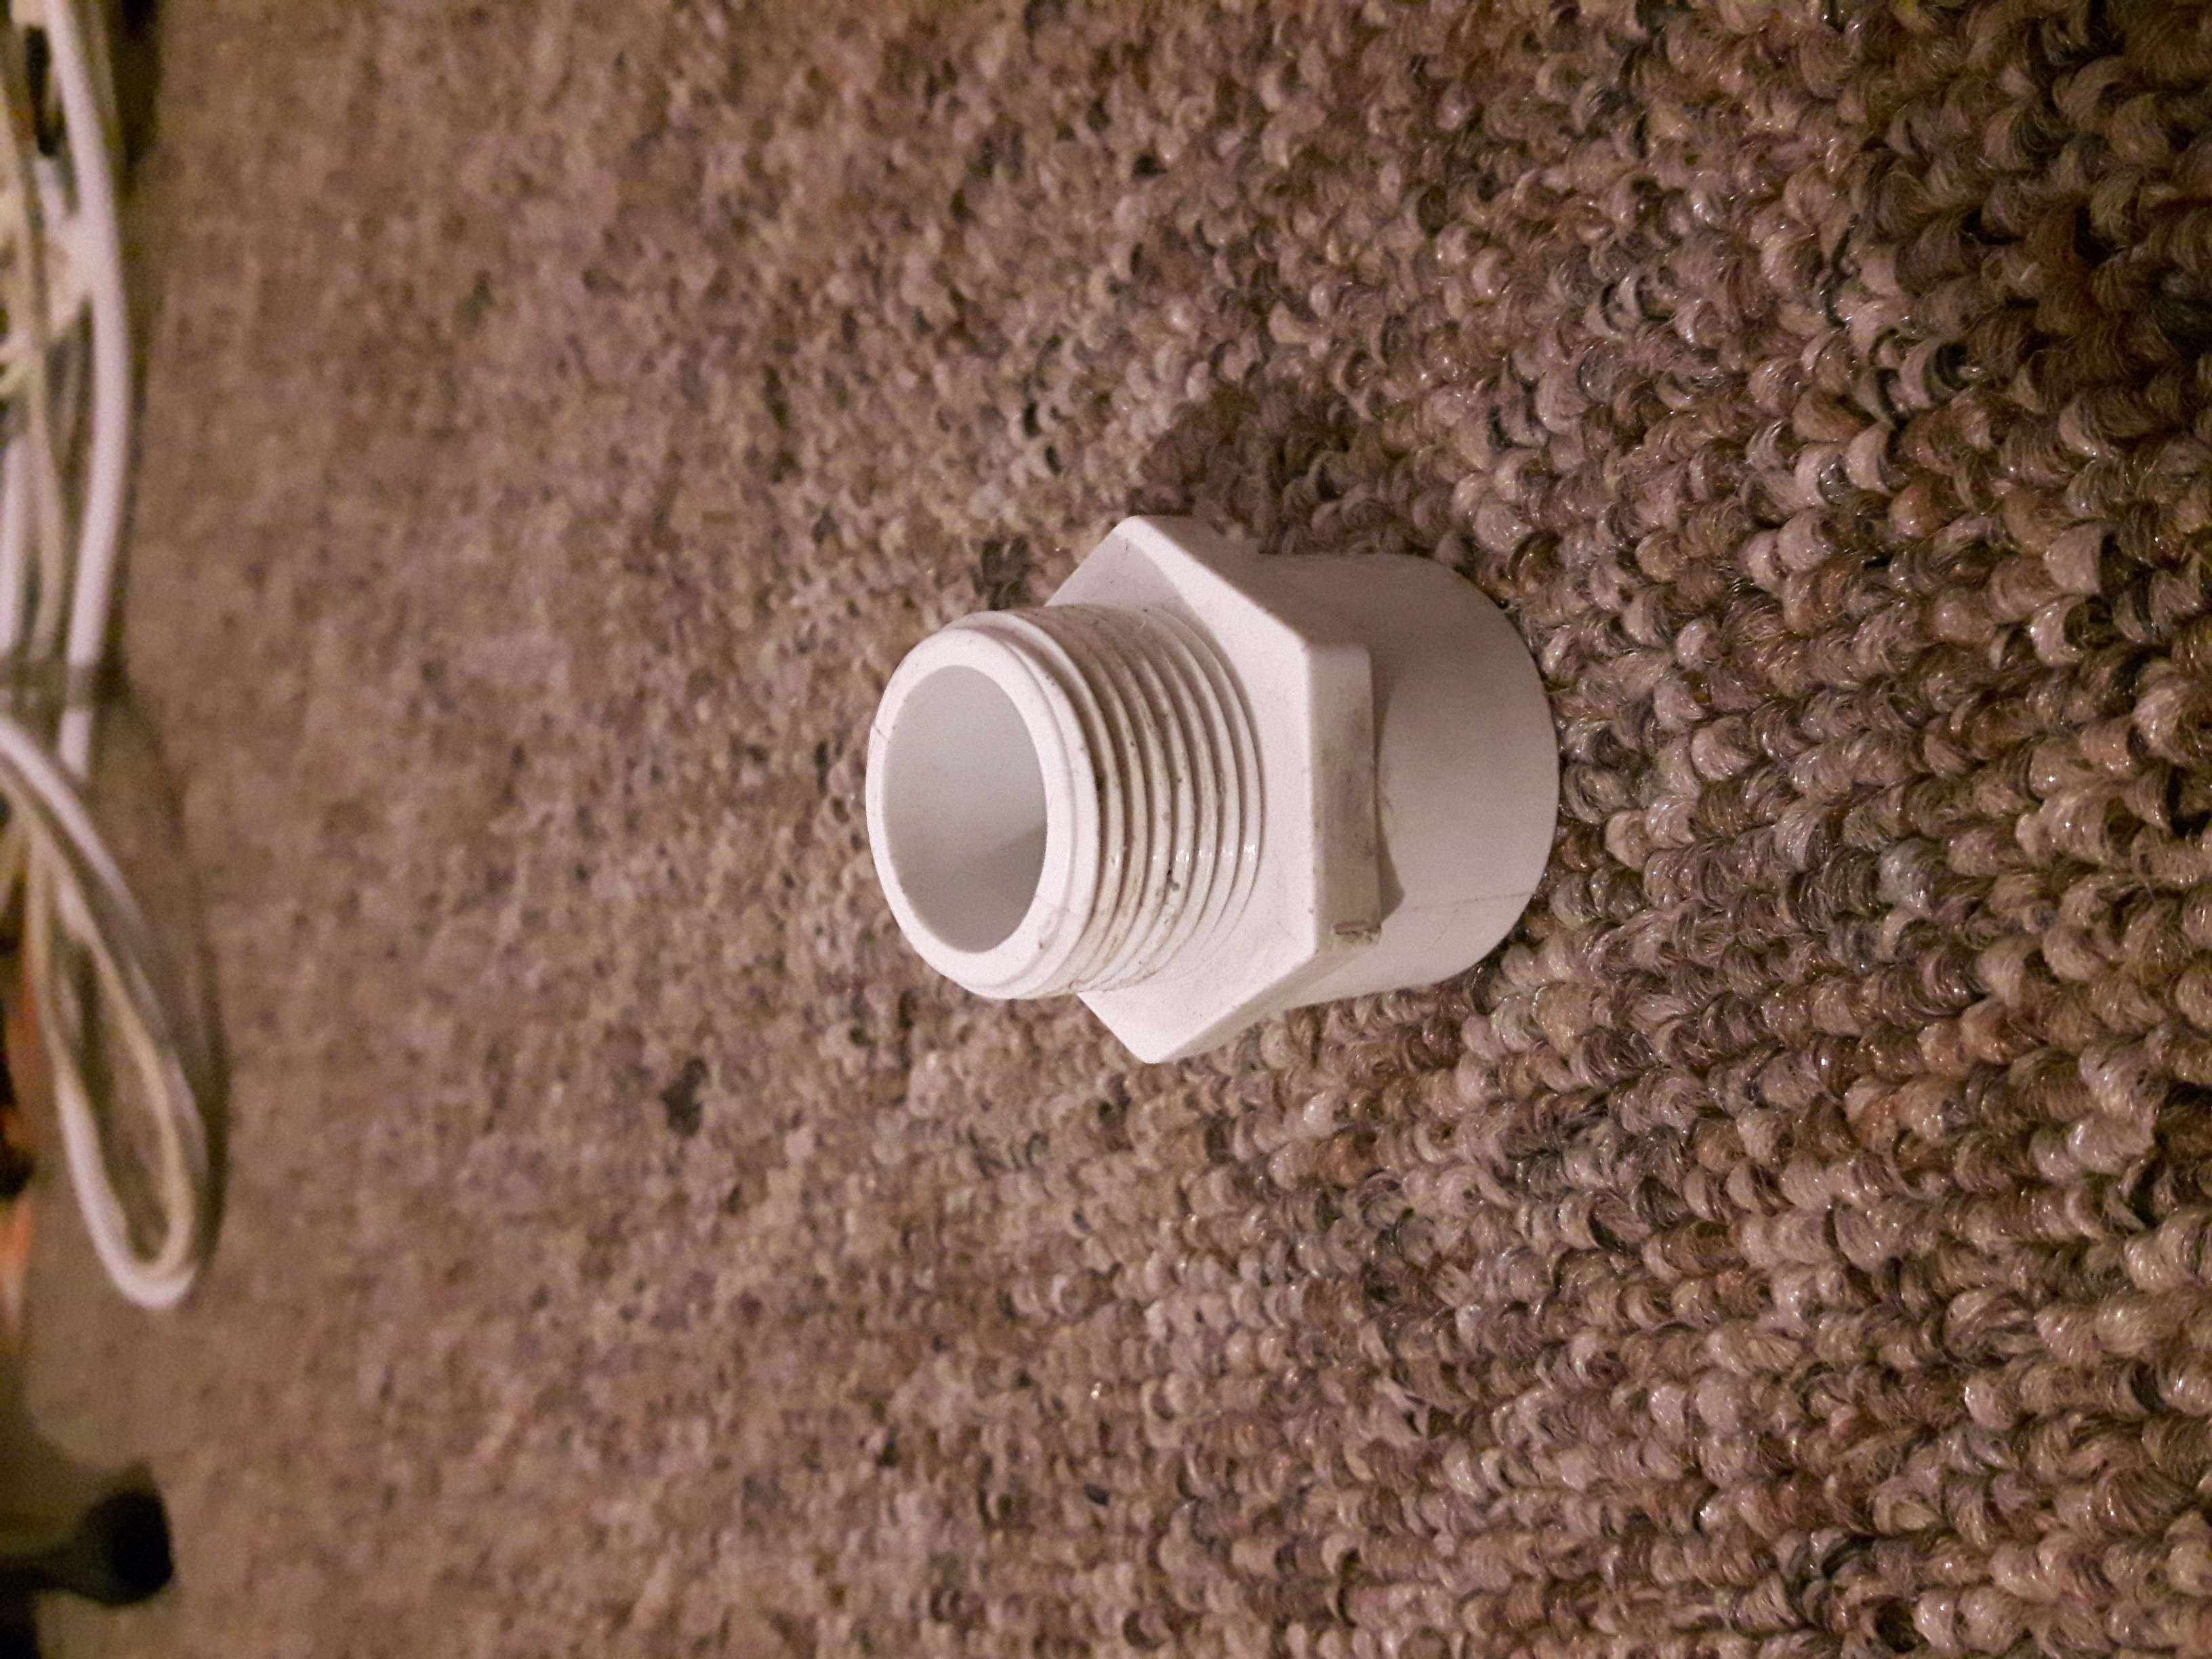
\includegraphics[width=\linewidth,angle=270]{20160826_213152.jpg}
\end{minipage}
\caption{Male part of the PVC connector through which the umbilical tether is threaded and then laminated.}
\label{fig:pvcConnector}
\end{figure}

\begin{figure}[htb]
\begin{center}
\begin{tabular}{c}
	\subfloat[Motor wires]
		{\includegraphics*[width=0.8\textwidth]{20160319_134634.jpg}
		\label{fig:strippingWires:label:a} } \\
	\subfloat[CAT5 cable]
		{\includegraphics*[width=0.8\textwidth]{20160319_131255.jpg}
		\label{fig:strippingWires:label:b} } \\
\end{tabular}
\end{center}
\caption{External cover of the wires is stripped so that less water drips through the umbilical connector once the wires are laminated in place.}
\label{fig:strippingWires}
\end{figure}

\begin{figure}[htb]
\begin{center}
\begin{tabular}{c c}
	\includegraphics*[width=0.6\textwidth,angle=270]{20160319_152814.jpg} & \includegraphics*[width=0.6\textwidth,angle=270]{20160319_153034.jpg} \\
\end{tabular}
\end{center}
\caption{Before laminating the wires into the PVC connector, they are separated to make sure some resin surrounds every wire and makes a~seal.}
\label{fig:separatingTheWires}
\end{figure}

\clearpage % Place these figures close to the text.

%-------------------------------------------------------------------------------
\subsection{Tether}\label{ssection:tether}
The umbilical tether consists of a~CAT5 cable, which extends the USB bus from the shore-based laptop to the ROV, as well as a~\unit[16]{A}-rated, three-chord power cable, which delivers battery power to the vehicle and grounds its structure. These two cables are held together by a~\unit[6]{mm} diameter nylon rope, which is tied around both cables at intervals of approximately one metre. The nylon rope can also be used to lift the vehicle or recover it from the water in case of failure. To this end, the nylon rope is mounted to the external steel structure of the ROV close to its centre of buoyancy. The steel structure provides a~strong mounting point, and the attachment location minimises the moments that the tether imparts on the vehicle, which makes it easier to operate. The location of the tether and the way it is attached to the ROV is shown in Fig.~\ref{fig:thetherOverview}.

During the initial towing tank test, described in section~\ref{section:manoeuvringTests}, it was discovered that the tether was too heavy and thus caused the ROV to sink, even though it was first made neutrally-buoyant on its own. To remedy this, bubble wrap was tied around the tether to increase its buoyancy. The bubble wrap was fixed with water-proof duct tape, as can be seen in Fig.~\ref{fig:thetherOverview}.

\begin{figure}[htb]
\begin{minipage}[b]{1\linewidth}
  \centering
	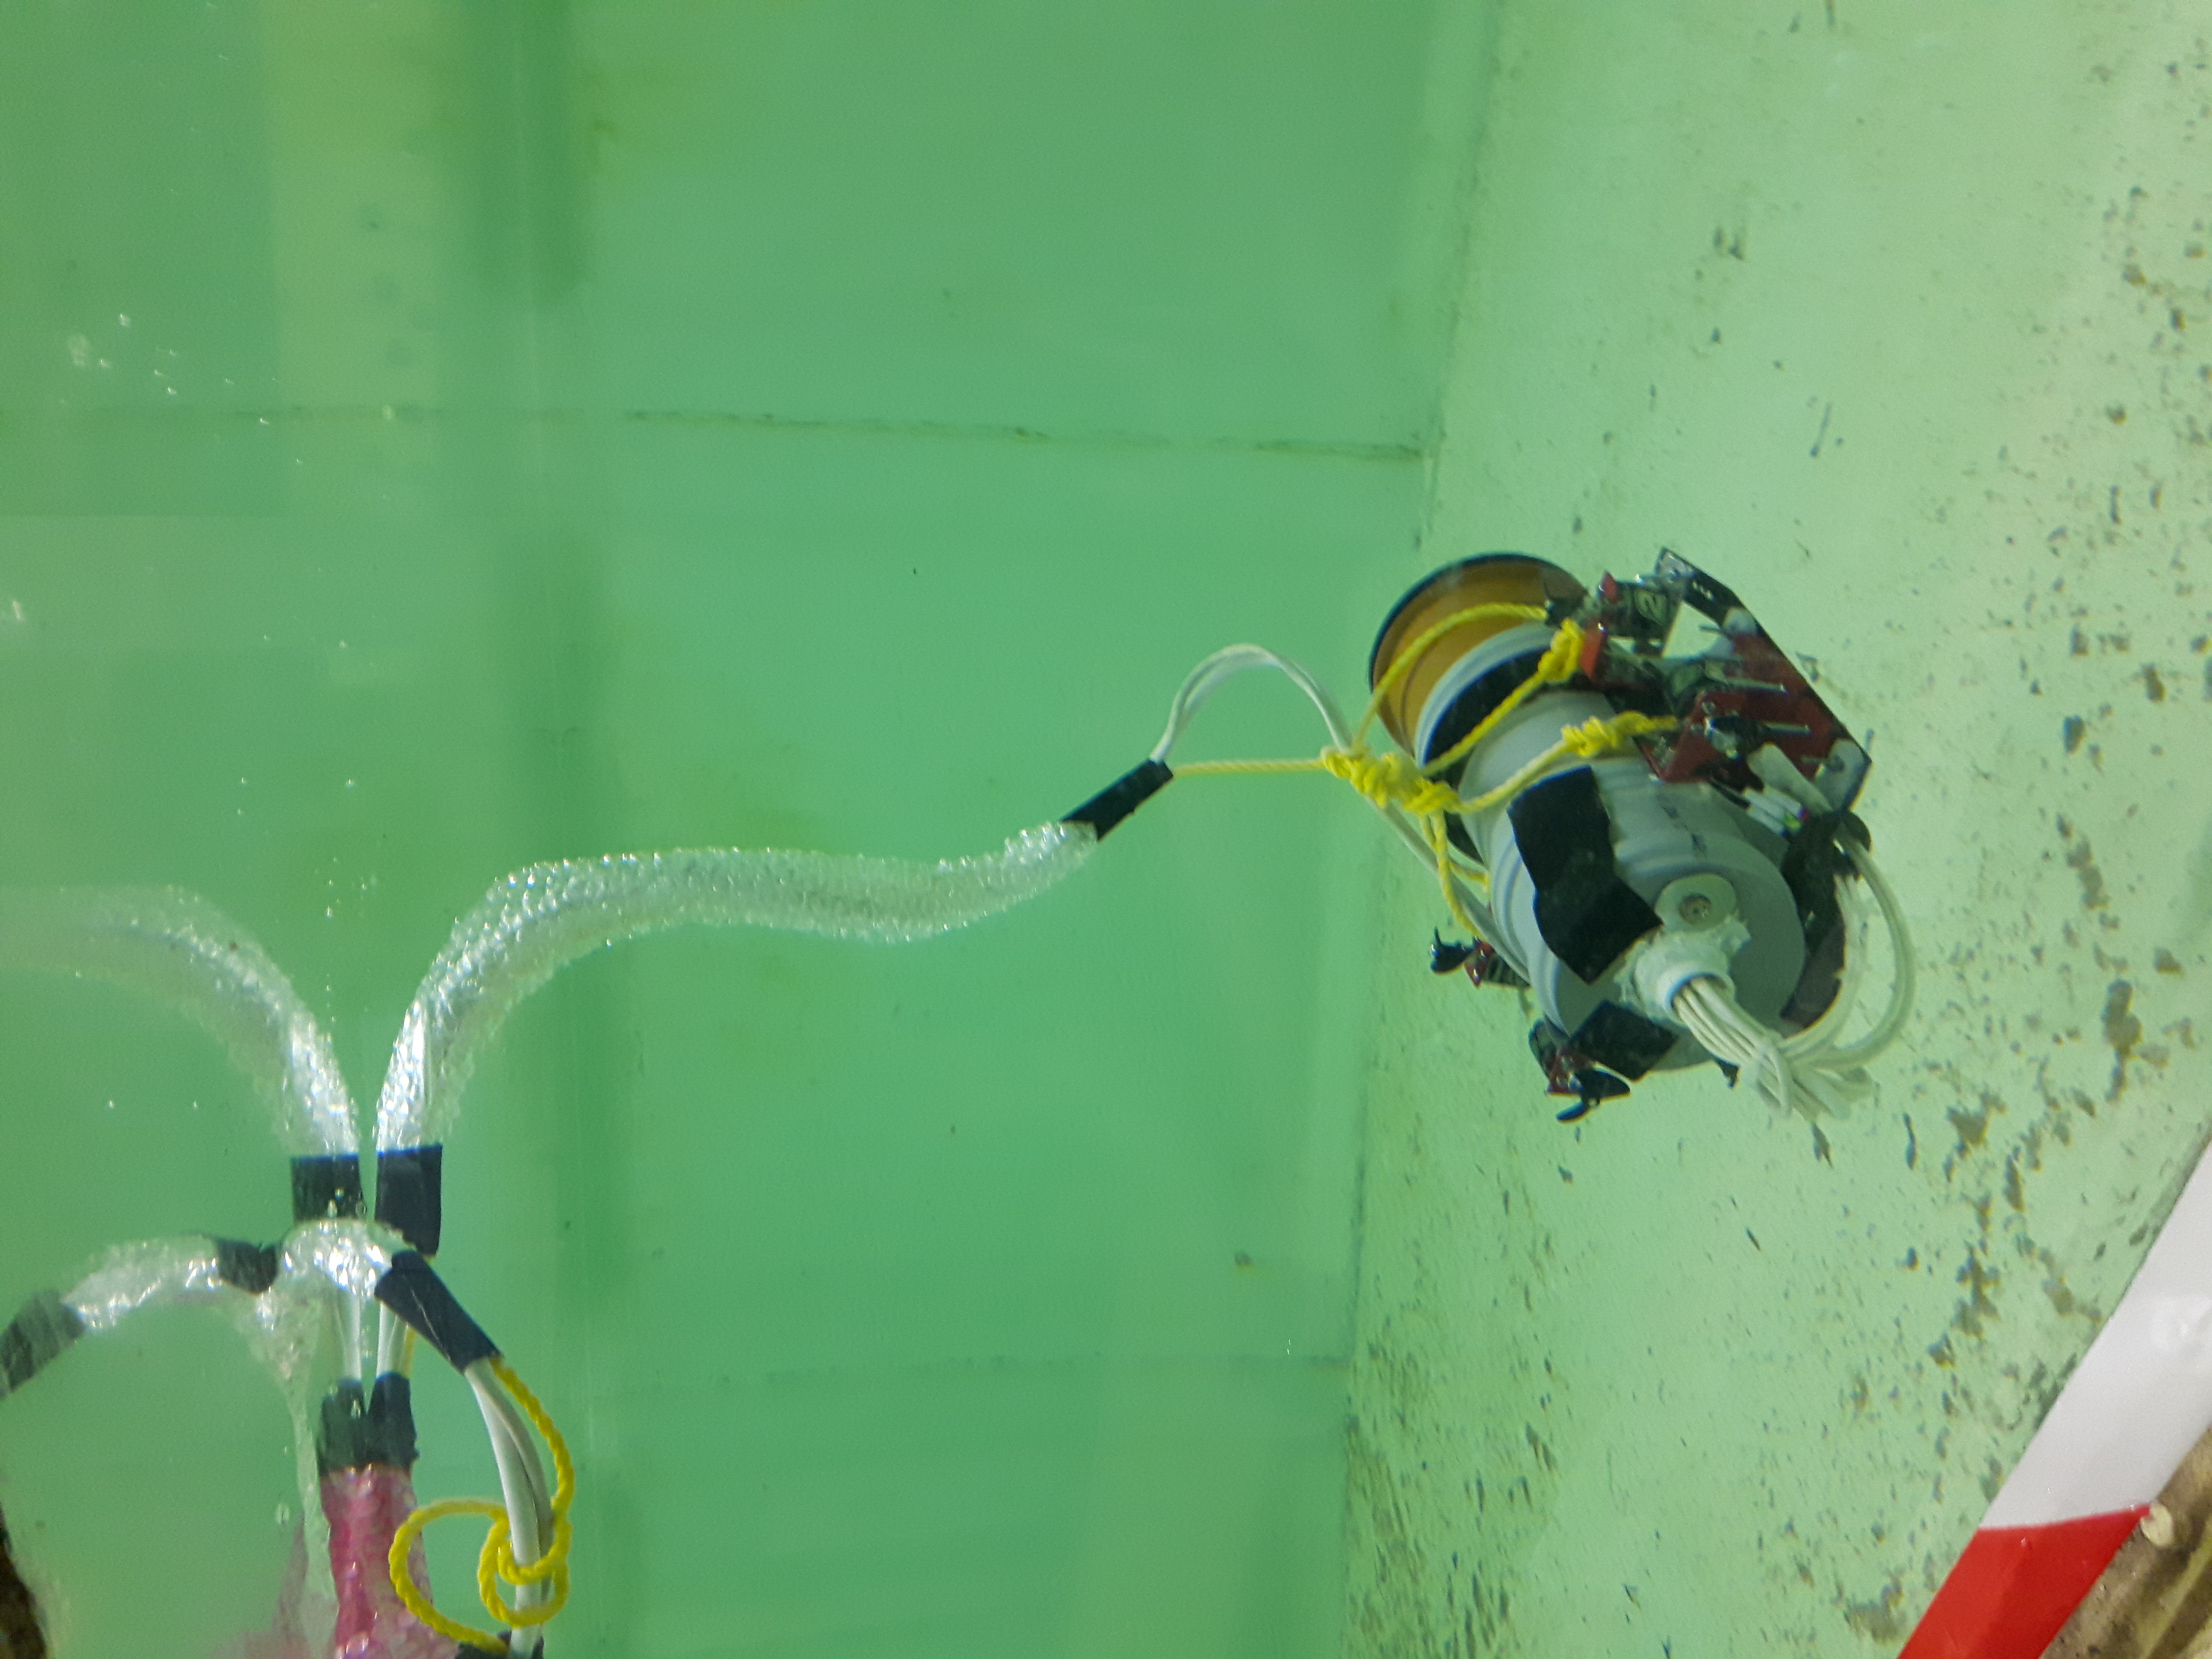
\includegraphics[width=\linewidth,angle=270]{20160826_135321.jpg}
\end{minipage}
\caption{Overview of the tether structure together with its attachment to the external steel structure.}
\label{fig:thetherOverview}
\end{figure}

\clearpage % Avoid "too many unprocessed floats" error.
